\documentclass{vldb}
\usepackage{graphicx}
\usepackage{caption}
\usepackage{subcaption}
\usepackage{multirow,booktabs}
%\usepackage{balance} 
\usepackage{epstopdf}
\usepackage{pbox}
\usepackage{url}
\let\proof\relax
\let\endproof\relax
\usepackage{algorithm, algpseudocode, amsmath,amsthm,amssymb}

\graphicspath{ {./charts/}, {./exp/} }
\epstopdfsetup{outdir=./charts/}
\newcommand{\reminder}[1]{ {\mbox{$<==$}} [[[ { \bf #1 } ]]] {\mbox{$==>$}}}
\newtheorem{definition}{Definition}
\newtheorem{theorem}{Theorem}
\newtheorem{example}{Example}
\DeclareMathOperator*{\argmin}{argmin}
\DeclareMathOperator*{\argmax}{argmax}
\DeclareMathOperator*{\triu}{triu}
\DeclareMathOperator*{\range}{range}
\newcommand*{\argminl}{\argmin\limits}
\newcommand*{\argmaxl}{\argmax\limits}
\newcommand{\eat}[1]{}
\newtheorem{lemma}[theorem]{Lemma}

\hyphenation{op-tical net-works semi-conduc-tor}

\begin{document}

% ****************** TITLE ****************************************

\title{A General and Parallel Platform for Mining Co-Movement Patterns over Large-scale Trajectories}

% ****************** AUTHORS **************************************

% You need the command \numberofauthors to handle the 'placement
% and alignment' of the authors beneath the title.
%
% For aesthetic reasons, we recommend 'three authors at a time'
% i.e. three 'name/affiliation blocks' be placed beneath the title.
%
% NOTE: You are NOT restricted in how many 'rows' of
% "name/affiliations" may appear. We just ask that you restrict
% the number of 'columns' to three.
%
% Because of the available 'opening page real-estate'
% we ask you to refrain from putting more than six authors
% (two rows with three columns) beneath the article title.
% More than six makes the first-page appear very cluttered indeed.
%
% Use the \alignauthor commands to handle the names
% and affiliations for an 'aesthetic maximum' of six authors.
% Add names, affiliations, addresses for
% the seventh etc. author(s) as the argument for the
% \additionalauthors command.
% These 'additional authors' will be output/set for you
% without further effort on your part as the last section in
% the body of your article BEFORE References or any Appendices.
%
%\author{
%	Qi Fan,
%	Dongxiang Zhang,
%	Huayu Wu,
%	Kian-Lee Tan
%}

\maketitle

\begin{abstract}
%With the advances of modern positioning technologies, tremendous trajectory data are nowadays become widely available. Discovering insightful information out of such large-scale trajectories is  important. Previous researches 
%have identified several interesting co-movement patterns and showcased their usefulness. However, we observe two challenges in applying them over large-scale trajectories. First, there is lack of a uniform definition of co-movement pattern, which makes it cumbersome to design a tailored solution to feed different needs. Second, existing works are all centralized schemes which are failed to scale to hundreds of millions of trajectories. 
%
%Motivated by this, in this paper, we present our novel solution on detecting co-movement patterns over large-scale trajectories. First, we model a general co-movement pattern (GCMP) to capture co-moving behaviors of objects. GCMP is versatile in representing all existing patterns by introducing a \emph{gap} constraints. With the gap, GCMP is also free from the so-called \emph{loose-connection} anomaly which appears in existing methods. Second, we resort to MapReduce for a parallel GCMP mining solution.
%%
%% We design a Temporal Replication and Parallel Mining (TRPM) method by replicating and grouping neighboring snapshots for effective parallelism. 
%We propose a novel Star Partition and ApRiori Enumerator (SPARE) to facilitate efficient parallelism. In SPARE, we model the pair-wised connections between objects as an Aggregate Graph and partition the graph into stars. Such a partition scheme guarantees no duplicate patterns are found from different partitions. For each star, SPARE employs an ApRiori Enumerator to systemically detect all valid GCMPs. As the traditional \emph{monotonicity} property in Apriori no longer holds, we develop the temporal based \emph{monotonicity} property to support efficient enumeration. We experiments our SPARE detector on three real datasets upto 200 million points using Apache Spark. The results show that SPARE achieves 90 times efficiency than centralized schemes and 10 times efficiency than a parallel baseline. Our experiments also demonstrates an almost linear scalability.

Discovering co-movement patterns from large-scale trajectory databases is an important mining task and has a wide spectrum of applications. Previous studies have identified several types of interesting co-movement patterns and showcased their usefulness. In this paper, we make two key contributions to this research field. First, we propose a more general co-movement pattern to unify those defined in the past literature. Second, we propose two types of parallel and scalable frameworks and deploy them on Spark. To the best of our knowledge, this is the first work to mine co-movement patterns in a trajectory database with hundreds of millions of points. Experiments on three large-scale trajectory datasets verified the efficiency and scalability of our proposed solutions.
\end{abstract}



\section{Introduction}
The prevalence of positioning devices has drastically boosted 
the scale and spectrum of trajectory collection to an unprecedented level. 
Tremendous amounts of trajectories, in the form of sequenced spatial-temporal 
records, are continually generated from animal telemetry chips, 
vehicle GPSs and wearable devices. Data analysis on large-scale 
trajectories benefits a wide range of applications and services, 
including traffic planning~\cite{zheng2011urban}, animal analysis~\cite{li2010miningperiodic}, and social recommendations~\cite{bao2013survey}, to name just a few.


A crucial task of data analysis on top of trajectories is 
to discover co-moving patterns. A \emph{co-movement} pattern~\cite{li2013managing} 
refers to a group of objects traveling together for a certain period of time 
and the group is normally determined by spatial proximity. 
A pattern is prominent if the size of the group exceeds $M$ and the length of the duration exceeds $K$, where $M$ and $K$ are parameters specified by users. Rooted from such basic definition 
and driven by different mining applications, there are a bunch of variants 
of co-movement patterns that have been developed with more advanced constraints.

Table~\ref{tbl:existing_co_patterns} summarizes several popular co-moving pattern s 
with different constraints in the attributes of clustering in spatial proximity,
consecutiveness in temporal duration and computational complexity. 
In particular,  the \emph{flock}~\cite{gudmundsson2006flock} 
and the \emph{group}~\cite{wang2006grouppattern} patterns require 
all the objects in a group to be enclosed by a disk with radius $r$; 
whereas the \emph{convoy}~\cite{jeung2008convoy}, the \emph{swarm}~\cite{li2010swarm} 
and the \emph{platoon}~\cite{li2015platoon} patterns resort to density-based 
spatial clustering. 
In the temporal dimension, the \emph{flock}~\cite{gudmundsson2006flock} 
and the \emph{convoy}~\cite{jeung2008convoy} require all the timestamps 
of each detected spatial group to be consecutive, which is referred to as \emph{global consecutiveness}; 
whereas the \emph{swarm}~\cite{li2010swarm} does not impose any restriction. 
The \emph{group}~\cite{wang2006grouppattern} and the \emph{platoon}~\cite{li2015platoon} adopt a compromised manner by allowing
arbitrary gaps between the consecutive segments, which is called \emph{local consecutiveness}. 
They introduce a parameter $L$ to control the minimum length of each local consecutive segment.


\begin{table} \scriptsize
\centering
\begin{tabular}{|c|c|c|c|}
\hline 
Patterns & {\tiny Proximity} & {\tiny Consecutiveness} & {\tiny Time Complexity}\\ 
\hline 
flock~\cite{gudmundsson2004flock} & disk-based &  global & $O(|\mathbb{O}||\mathbb{T}|(M + log(|\mathbb{O}|))$ \\ 
\hline 
convoy~\cite{jeung2008convoy} & density-based &   global & $O(|\mathbb{O}|^2+|\mathbb{O}||\mathbb{T}|)$\\ 
\hline 
swarm~\cite{li2010swarm} & density-based  & - & $O(2^{|\mathbb{O}|}|\mathbb{O}||\mathbb{T}|)$  \\ 
\hline 
group~\cite{wang2006grouppattern} & disk-based &  local & $O(|\mathbb{O}|^2|\mathbb{T}|)$ \\ 
\hline 
platoon~\cite{li2015platoon} & density-based &  local & $O(2^{|\mathbb{O}|}|\mathbb{O}||\mathbb{T}|)$\\ 
\hline 
\end{tabular} 
\caption{Constraints and complexity of co-movement patterns. The time complexity indicates the performance in the worst case, where $|\mathbb{O}|$ is the total number of objects and $|\mathbb{T}|$ is the number of descritized timestamps.}
\label{tbl:existing_co_patterns}
\end{table}




\begin{figure}[h]
\centering
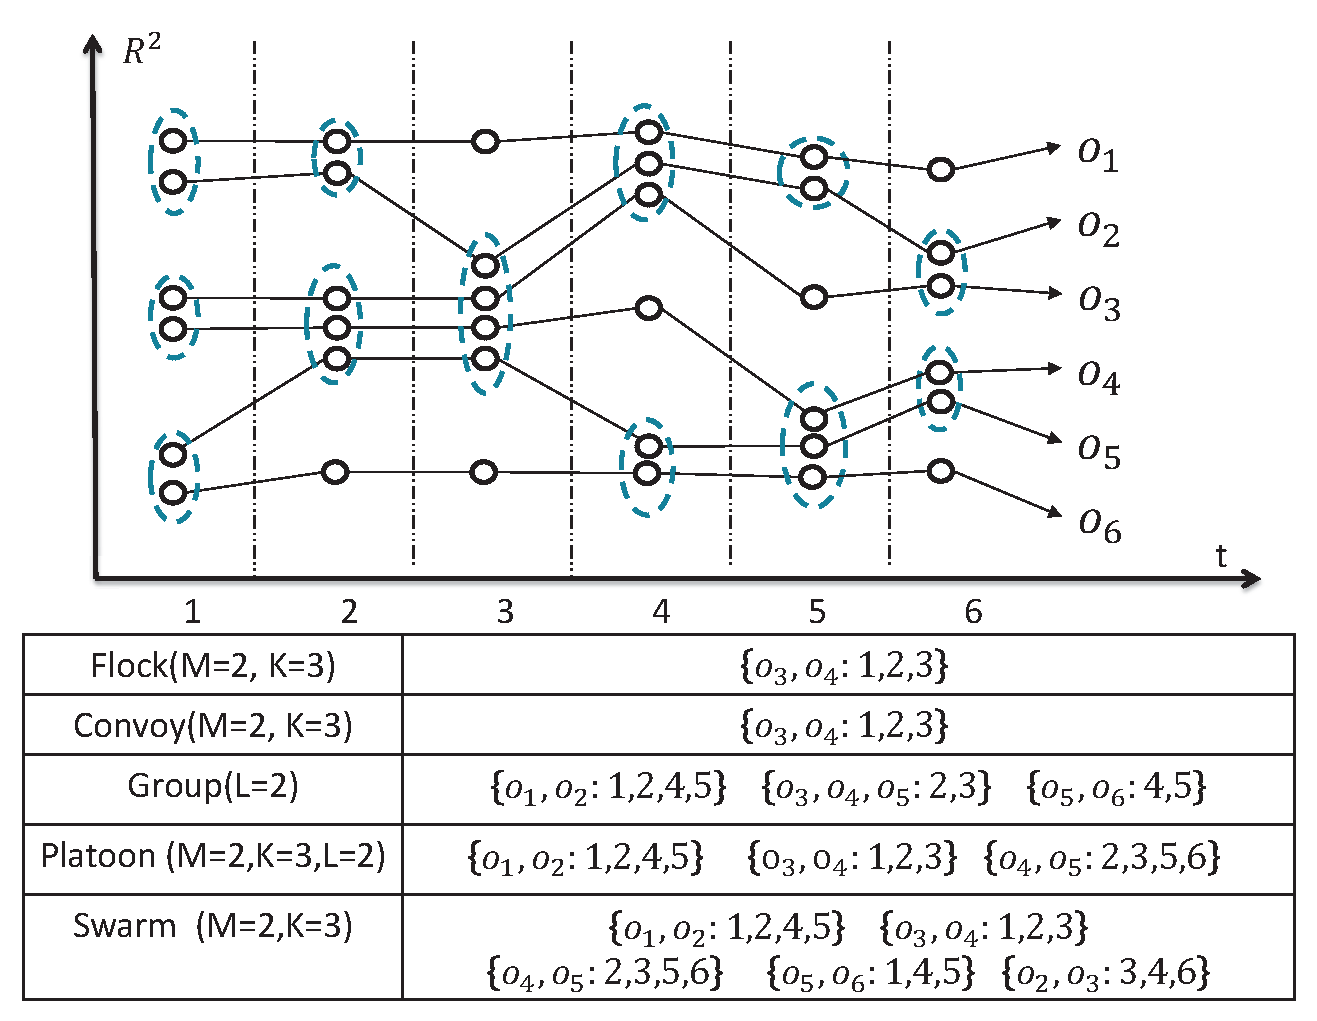
\includegraphics[width=0.45\textwidth]{related_work.eps}
\caption{Trajectories and co-movement patterns; The example consists of six trajectories across six snapshots. Objects in spatial clusters are enclosed by dotted circles. $M$ is the minimum cluster cardinality; $K$ denotes the minimum number of snapshots for the occurrence of a spatial cluster; and $L$ denotes the minimum length for local consecutiveness.}
\label{fig:related_work}
\end{figure}

Figure~\ref{fig:related_work} is an example to demonstrate the concepts of various co-movement patterns. The trajectory database consists of six moving objects and the temporal dimension is discretized into six snapshots. In each snapshot, we treat the clustering methods as a black-box and assume that they generate the same clusters. Objects in proximity are grouped in the dotted circles. As aforementioned, there are three parameters to determine the co-movement patterns and the default settings in this example are $M=2$, $K=3$ and $L=2$. Both the \emph{flock} and the \emph{convoy} require the spatial clusters to last for at least $K$ consecutive  timestamps. Hence,$\{o_3,o_4\}$ and $\{o_5,o_6\}$  remains the only two candidates matching the patterns. The \textit{swarm} relaxes the pattern matching by discarding the temporal consecutiveness constraint. Thus, it generates many more candidates than the \textit{flock} and the \textit{convoy}. The \textit{group} and the \textit{platoon} add another constraint on local consecutiveness to retain meaningful patterns. For instance, $\{o_1,o_2:1,2,4,5\}$ is a pattern matching local consecutiveness because timestamps $\{1,2\}$ and $\{4,5\}$ are two segments with length no smaller than $L=2$. The difference between the \textit{group} and the \textit{platoon} is that the \textit{platoon} has an additional parameter $K$ to specify the minimum number of snapshots for the spatial clusters. This explains why $\{o_3,o_4,o_5:2,3\}$ is a  \textit{group} pattern but not a \textit{platoon} pattern.

As can be seen, there are various co-movement patterns requested by different applications and it is cumbersome to design a tailored solution for each type. In addition, despite the generality of the \emph{platoon} (i.e., it can be reduced to other types of patterns via proper parameter settings), it suffers from the so-called \emph{loose-connection} anomaly. We use two objects $o_1$ and $o_2$ in Figure~\ref{fig:platoon_weakpoint} as an example to illustrate the scenario. These two objects form a \emph{platoon} pattern in timestamps $\{1,2,3,102,103,104\}$. However, the two consecutive segments are $98$ timestamps apart, resulting in a false positive co-movement pattern. In reality, such an anomaly may be caused  by the periodic movements of unrelated objects, such as vehicles stopping at the same petrol station or animals pausing at the same water source. 
Unfortunately, none of the existing patterns have directly addressed this anomaly.


%As can be seen, there are various co-movement patterns requested by different 
%applications and it is cumbersome to design a tailored solution for each type. 
%As pointed in \cite{li2015platoon, li2010swarm}, stringent temporal constraints (e.g., global consecutiveness on \emph{flock} and \emph{convoy}) may miss out many interesting patterns. However, we 
%further observe that pattern definitions with overly-relaxed temporal constraints (e.g., \emph{swarm}, \emph{group} and \emph{platoon}) lose the fine control of a pattern which lead to noisy results and unnecessary computations. We name this scenario as \emph{loose-connection} anomaly. To illustrate, as shown in Figure~\ref{fig:platoon_weakpoint}, the two objects $o_1, o_2$ form a \emph{platoon} pattern 
%$\{o_1,o_2:1,2,3,102,103,104\}$. However, the consecutive segments are $98$ timestamps apart, 
%making the co-moving behavior very loose.
%In reality, such an anomaly is likely induced by the periodic movements of unrelated objects 
%such as, vehicles stopping at the same petrol station, animals pausing at the same water source etc.  Interestingly, none of the temporal-relaxed patterns (e.g., \emph{swarm}, \emph{group} and \emph{platoon}) are able to directly avoid such an anomaly.

%In addition, existing pattern definitions are not expressive enough and may miss 
%interesting patterns or return noisy results. We summarize 
%the two scenarios as \emph{missing-pattern} anomaly
%and \emph{loose-connection} anomaly.
%A \emph{missing-pattern} anomaly arises due to the stringent constraints on the pattern duration.
%As shown in Figure~\ref{fig:platoon_weakpoint} (a), if we set $K=4$, 
%neither \emph{flock}s nor \emph{convoy}s can be discovered. This is because
%$o_1$ is away from $o_2$ at timestamp $4$, which is likely caused by
%the traffic control or the clustering inaccuracy at time $4$. On the other hand,
%the \emph{loose-connection} anomaly occurs due to an over-relaxed constraint on 
%the duration. As shown in Figure~\ref{fig:platoon_weakpoint} (b),
%the two objects $o_1, o_2$ form a \emph{platoon} pattern 
%$\{o_1,o_2:1,2,3,102,103,104\}$. However, the consecutive segments are $98$ timestamps apart, 
%making the co-moving behavior very weak.
%In reality, such an anomaly is likely to be induced by the periodic movements of unrelated objects 
%such as, vehicles stopping at the same petrol station, animals pausing at the same water source etc. 
%It is easy to see that none of the existing co-movement patterns are able to avoid these two anomalies.

\begin{figure}[h]
\center
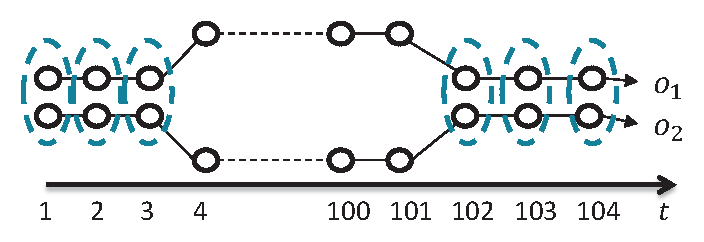
\includegraphics[width=0.35\textwidth]{platoon_weakpoint.eps}
\caption{\emph{Loose-connection} anomaly. Even though $\{o_1, o_2: 1,2,3,102,103,104\}$ is considered as a valid \emph{platoon} pattern, it is highly probable that these two objects are not related as the two consecutive segments  are 98 timestamps apart. 
% in \emph{platoon}, \emph{swarm} and \emph{group} results.
}
\label{fig:platoon_weakpoint}
\end{figure}

%In current literature,
%users are unable to explicitly exclude the loosely-connected patterns even when those patterns are unwanted.
%
%
% we summarize two anomalies 
%The \emph{missing-pattern}~\cite{li2010swarm} anomaly arises due to the stringent constraints on the duration of a pattern. As shown in 
%Figure~\ref{fig:platoon_weakpoint} (a).  As we notice, object $o_1$ is temporally far from $o_2$ at timestamp $4$, which is likely to be
%the result of errors in interpretation of missing points, or $o_1$ faces traffic control at time $4$. Such an anomaly can
%be resolved by \emph{swarm} and \emph{platoon} due to a relaxed constraint on the duration. However, 
%\emph{swarm} and \emph{platoon}'s relaxations encompass a type of non-interesting patterns which is referred
%as \emph{loose-connection}~\cite{li2015platoon} anomaly. 
%
%
%%This is because that \emph{platoon} allows the timestamps in a pattern duration to be in arbitrary distance, making the object group loosely
%connected. For instance, patterns with duration $\{1,2,100,101\}$ could be a valid \emph{platoon}; however, the two timestamps $2,100$ are too far from each other.

%For instance, PUT THE FIGURE AND EXPLANATION HERE.

%\begin{figure}[h]
%\center
%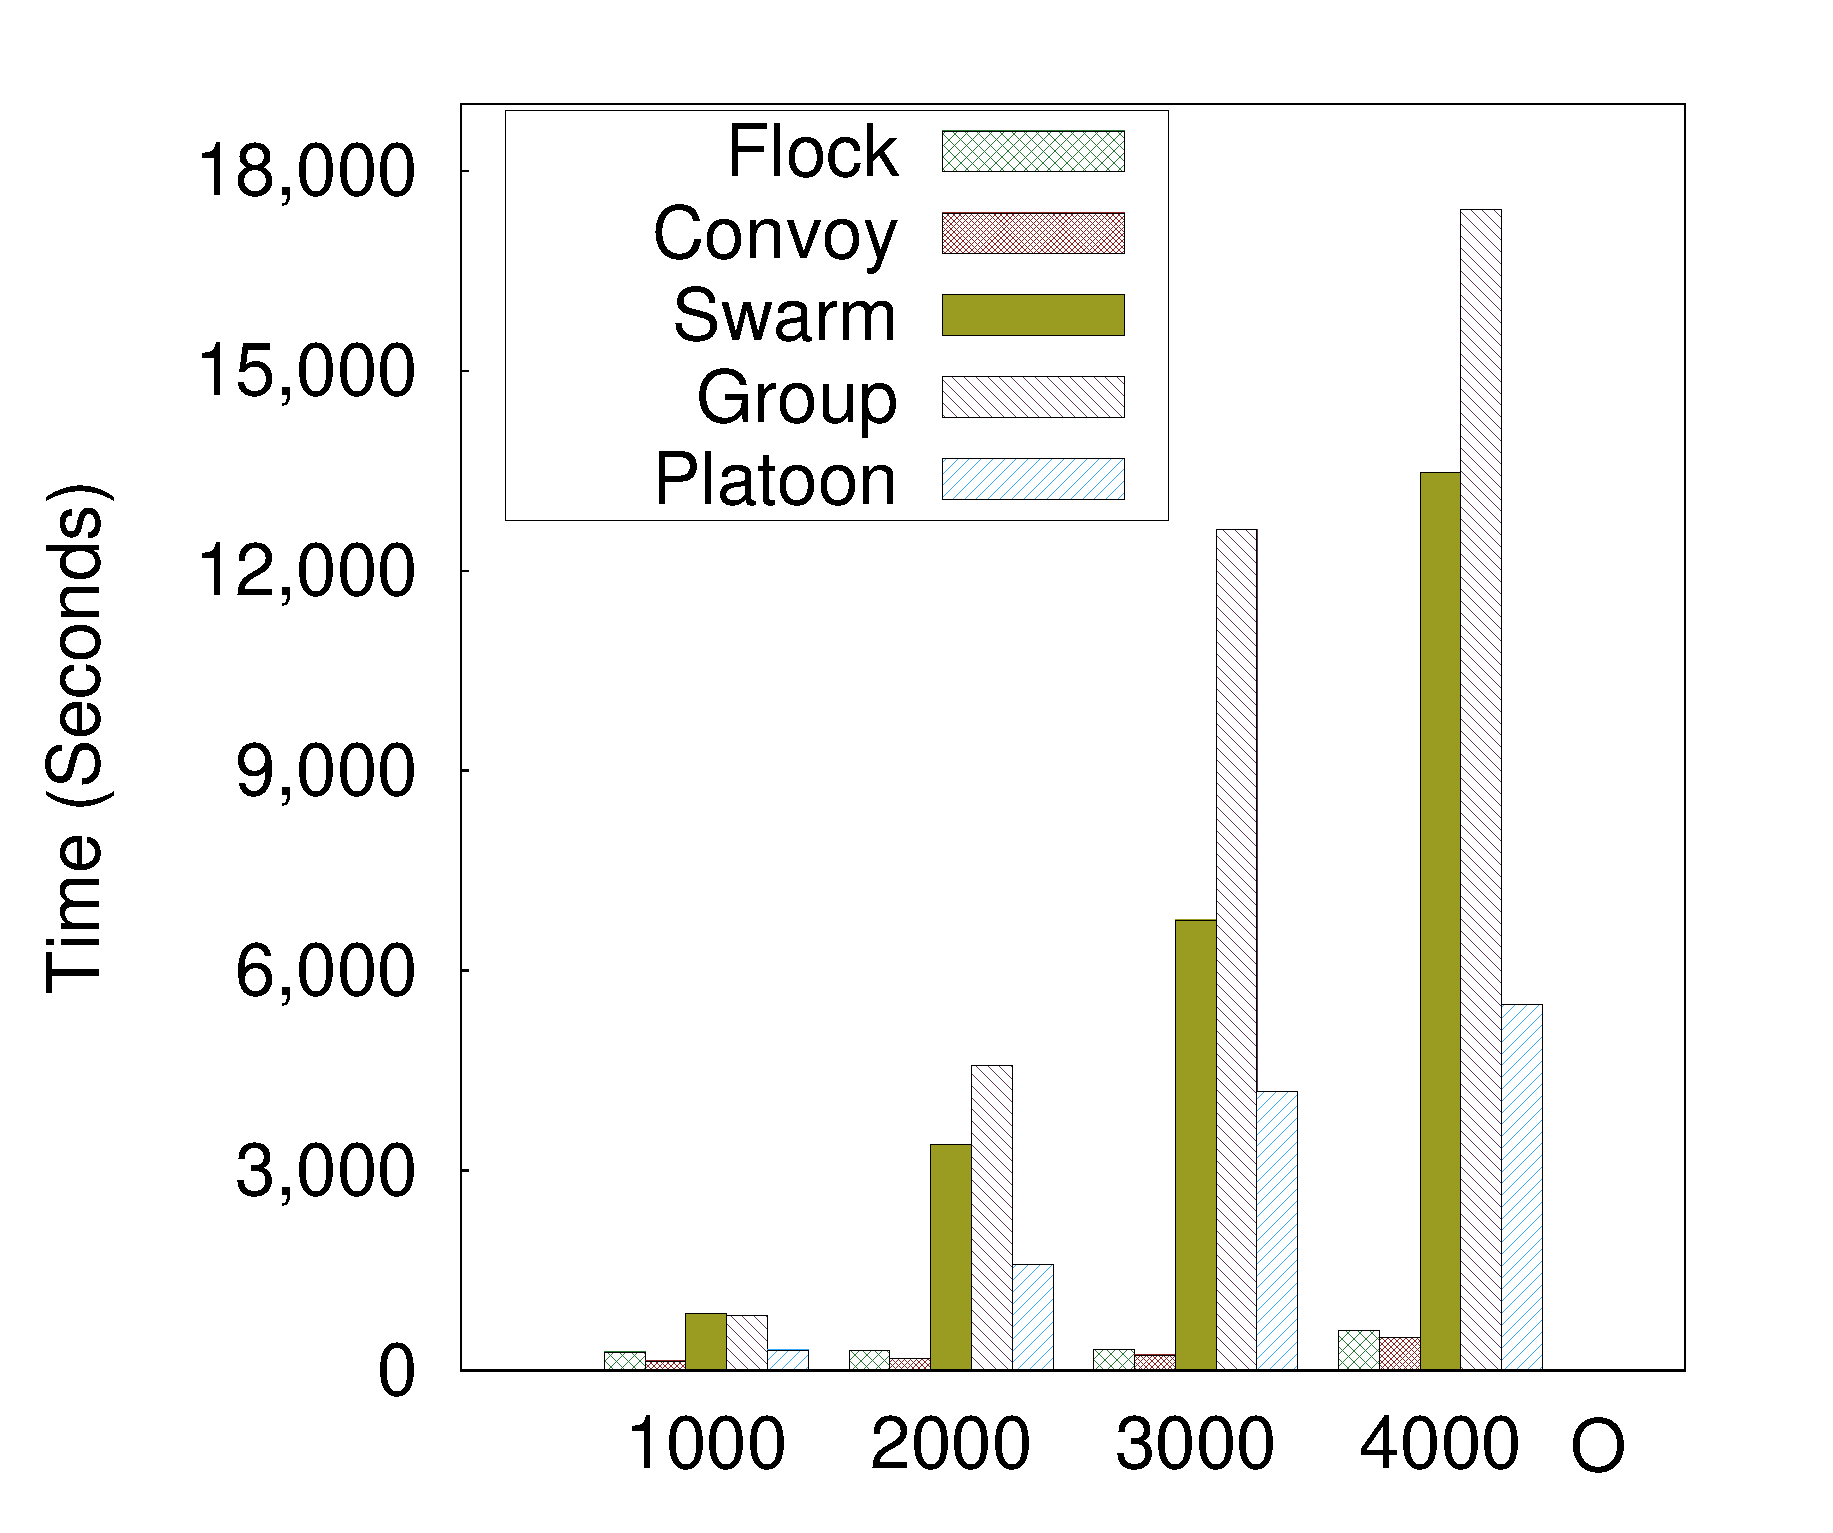
\includegraphics[width=0.35\textwidth]{rw_perf_O.eps}
%\caption{Two anomalies in existing patterns. (a) \emph{Missing-pattern} anomaly
%in \emph{flock} and \emph{convoy}. When $K=4$, none of the two patterns can be discovered. (b) \emph{Loose-connection} anomaly in \emph{platoon} and \emph{swarm}. The consecutive segment of $o_1$ and $o_2$ are 98 timestamps apart, however, the pattern $\{o_1, o_2: 1,2,3,102,103,104\}$ is included in platoon and swarm results.}
%\label{fig:platoon_weakpoint}
%\end{figure}


The other issue with existing methods is that they are built on top of centralized indexes which may not be scalable. Table~\ref{tbl:existing_co_patterns} shows their theoretical complexities in the worst cases and the largest real dataset ever evaluated in previous studies is up to million-scale points collected from hundreds of moving objects. In practice, the dataset is of much higher scale and the scalability of existing methods is left unknown. Thus, we conduct an experimental evaluation with $4000$ objects moving for $2500$ timestamps to examine the scalability. Results in Figure~\ref{fig:related_work_scalability} show that their performances degrade dramatically as the dataset scales up. For instance, the detection time of \emph{group} drops twenty times as the number of objects grows from \emph{1k} to \emph{4k}. Similarly,
the performance of \emph{swarm} drops over fifteen times as the number of snapshots grows from \emph{1k} to \emph{2.5k}.
These observations imply that existing methods are not scalable to support large-scale trajectory databases. 

%It is easy to spot that none of the existing solutions are scalable to handle large-scale trajectories which include near billions of data points.
%In fact, as shown in Table~, the mining of co-movement patterns require high complexity. For instance, the
%complexities of \emph{swarm} and \emph{platoon} are already exponential. 
%Therefore, none of them can handle millions of trajectories efficiently. 
%CAN YOU ANALYSE THEIR COMPLEXITY TO ADDRESS THE PROBLEM OF SCALABILITY.
\begin{figure}[h]
    \centering
    \begin{subfigure}[b]{0.23\textwidth}
            \centering
            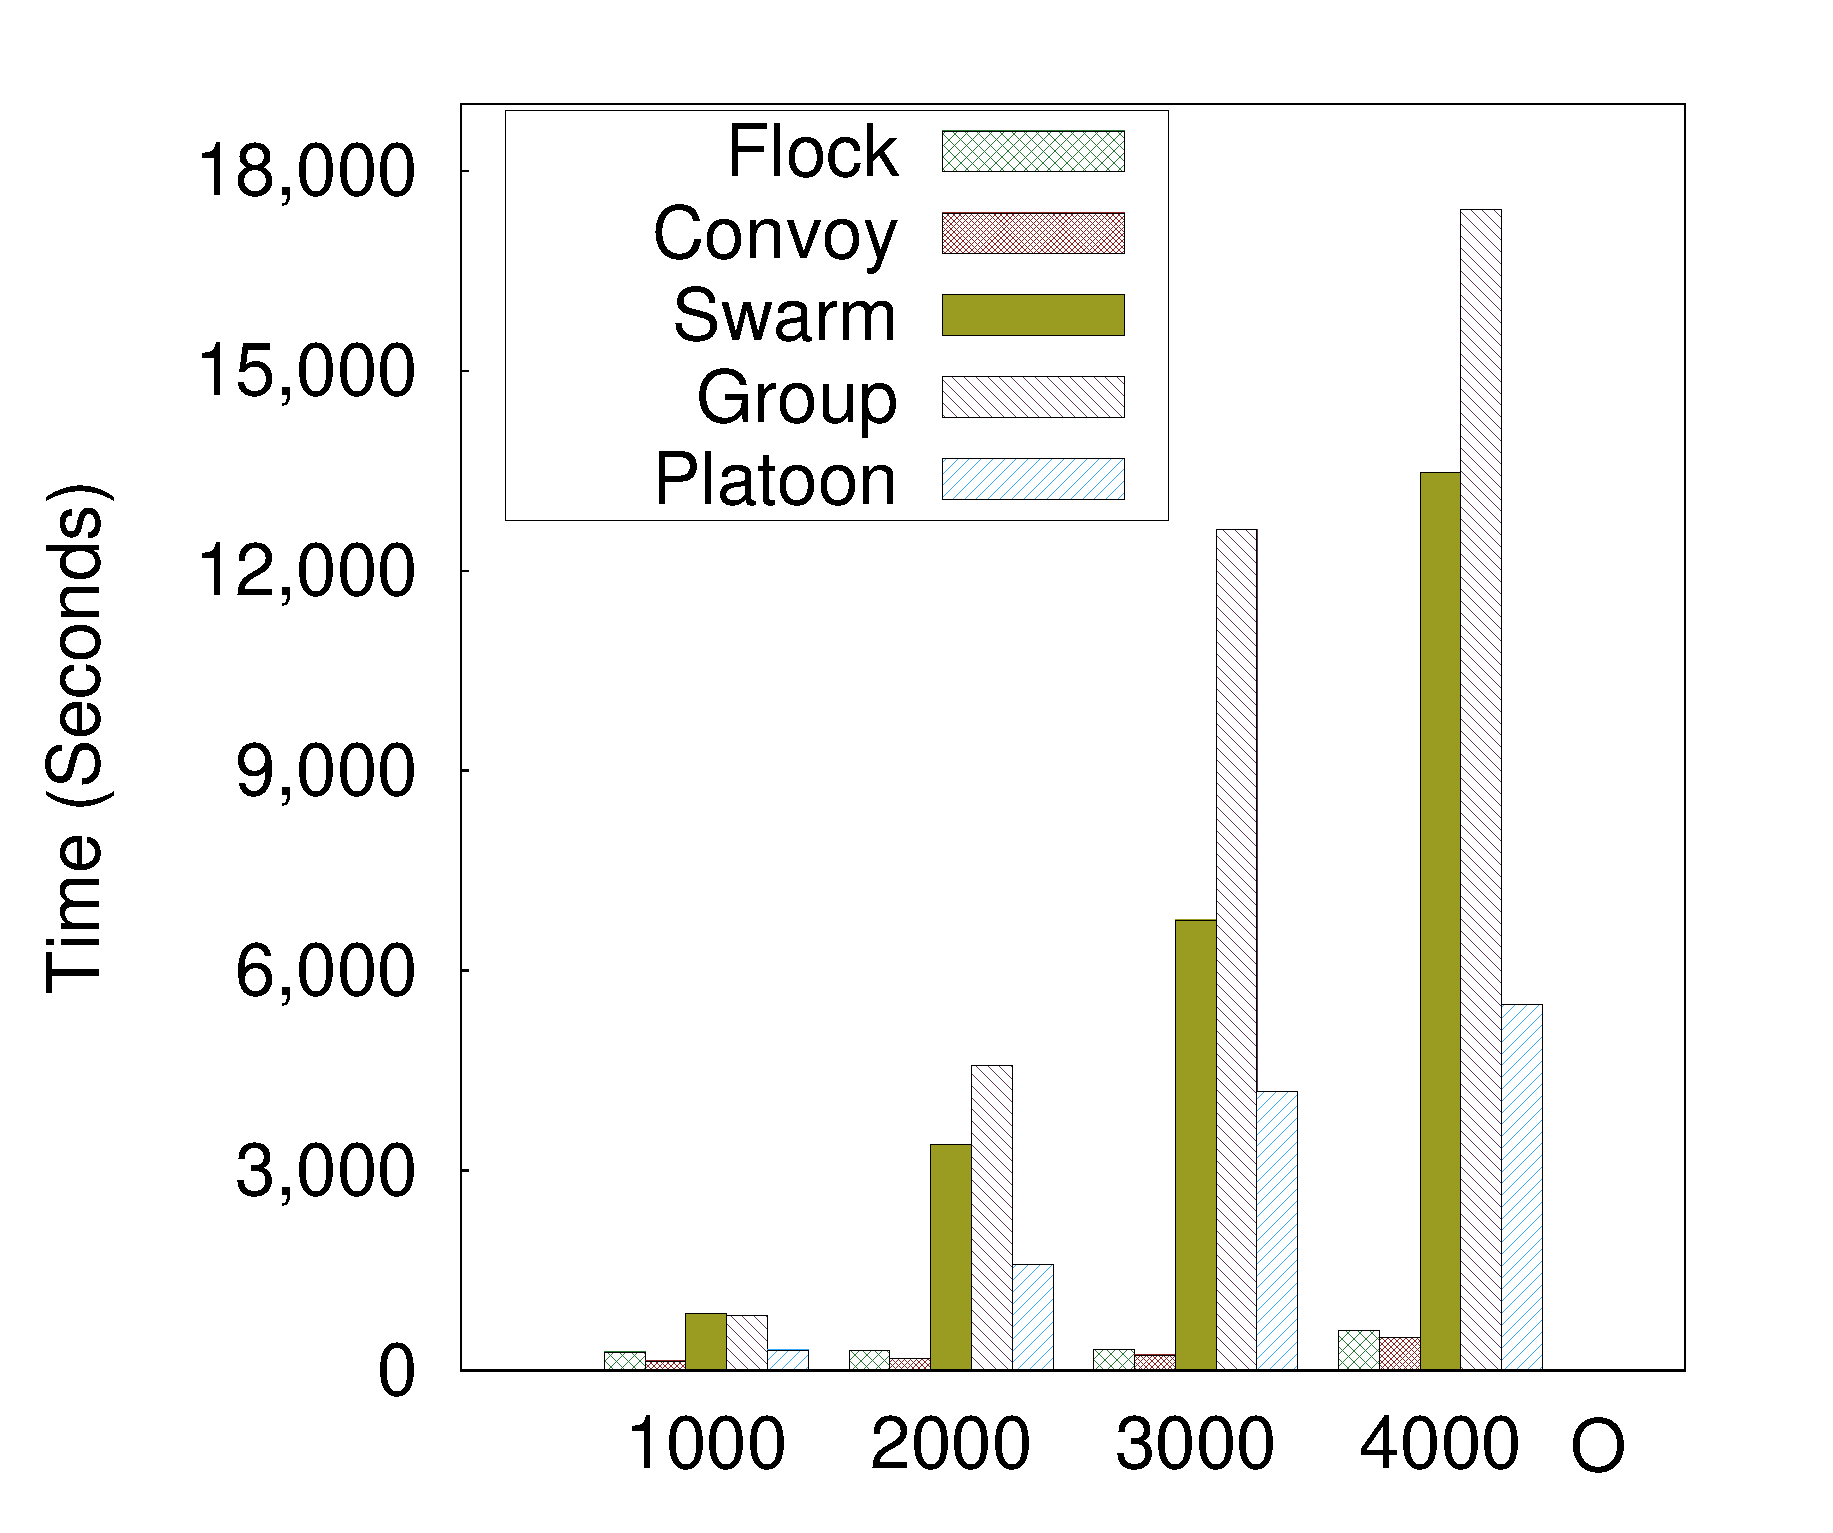
\includegraphics[width=\textwidth]{rw_perf_O.eps}
		\subcaption{$1k$ timestamps}
    \label{fig:fig1}
    \end{subfigure}
    \begin{subfigure}[b]{0.23\textwidth}
            \centering
            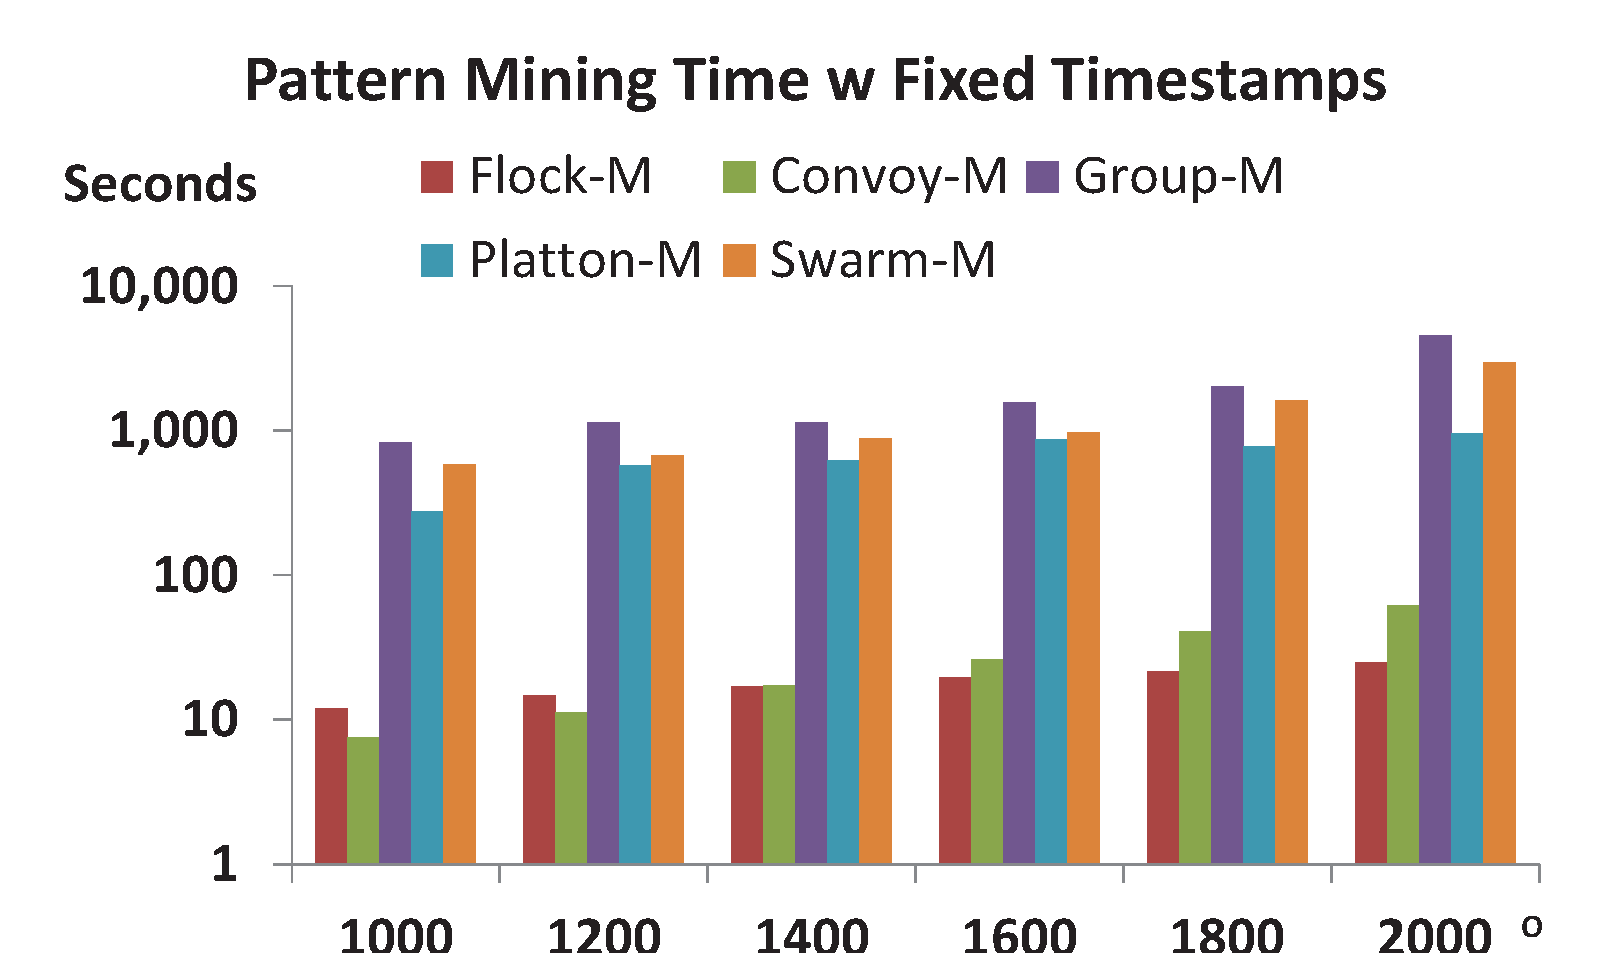
\includegraphics[width=\textwidth]{rw_perf_T.eps}
         \subcaption{$1k$ objects}
    \label{fig:fig2}
    \end{subfigure}
    \caption{Performance measures on existing co-movement patterns. A sampled Geolife data set
    is used with up two 2.4 million data points. Default parameters are $M=10$ $K=20$ $L=10$.}
    \label{fig:related_work_scalability}
\end{figure}




Therefore, our primary contributions in this paper are to close these two gaps. 
First, we propose the \emph{general co-movement pattern} (GCMP) which models
various co-moment patterns in a unified way and can avoid 
the \emph{loose-connection} anomaly. In GCMP, we introduce a new gap parameter $G$ to pose a constraint on the temporal gap between two consecutive segments. By setting a feasible $G$, the loose-connection anomaly can be avoided. In addition, our GCMP is both general and expressive. It can be reduced to any of the previous patterns by customizing the parameters.

%Therefore, users are 
%still able to exclude non-consecutive patterns 
%or include loosely-connected patterns when they feel necessary.


%We introduce the gap parameter $G$,
%When such loosely-connected patterns are unwanted, users currently are unable to directly control the outputs.
%To cope with both of the two anomalies, we propose 
%by introducing the gap parameter $G$, 

%By so doing, we gain a fine-grained control s, which As we show in later sections, the general co-movement pattern is able to express existing patterns by setting appropriate parameters. 
%IS IT POSSIBLE TO USE FIGURE 1 TO ADDRESS THE PROBLEM OF PLATOON, INSTEAD OF PROPOSING A NEW EXAMPLE SCENARIO?
%

Second, we investigate deploying our GCMP detector on MapReduce platforms (such as Hadoop and Spark) to tackle the scalability issue. Our technical contributions are three-fold. First, we replicate the snapshots in multiple data chunks to support efficient parallel processing. Second, we devise a novel \emph{Star Partition and Mining} (SPM) algorithm as a fine-granularity partitioning strategy to achieve workload balance. For each star, an Apriori method is adopted to mine the co-movement patterns. Third, we leverage the \emph{temporal monotonicity} property of GCMP to design several optimization techniques including \emph{edge-simplification} to prune initial candidates, \emph{temporal apriori pruning} and \emph{forward closure checking} to reduce the number of enumerated candidates in the Apriori algorithm.
%
%we propose two types of optimization techniques to further improve the performance, including \emph{edge-simplification} to boost the shuffle process and \emph{temporal monotonicity pruning} and 
%\emph{forward closure checking} to significantly reduce the number of enumerated candidates in the Aproiro algorithm.


We conduct a set of extensive experiments on three large-scaled real datasets with hundreds of millions 
temporal points. 
The results show that our parallel scheme efficiently supports GCMP mining in large datasets.
In particular, with near 200 million trajectory points, 
our scheme runs within 10 minutes using 135 cores. Whereas centralized solution takes near 7 hours for 
1 million trajectory points.
Moreover, our optimized SPM methods achieves upto XXX times efficiency
as compared to the baseline algorithm with near linear scalability.

The rest of our paper is organized as follows: Section~\ref{sec:related_works} summarizes the relevant literature on 
trajectory pattern mining. Section~\ref{sec:definition} states the problem definition of our general co-movement pattern mining. Section~\ref{sec:trm} provides a baseline solution. An advanced solution named
\emph{star partition and mining} is presented in Section~\ref{sec:spm}. Section~\ref{sec:opt} discusses various optimization techniques. Section~\ref{sec:exp} conducts extensive experiments to verify the efficiency of our system. Finally Section~\ref{sec:concl} concludes the paper.

\section{Related Works}
\label{sec:related_works}
The \emph{co-movement patterns} in literature consist 
of five members, namely \emph{group}~\cite{wang2006grouppattern}, \emph{flock}~\cite{gudmundsson2004flock},
\emph{convoy}~\cite{jeung2008convoy}, \emph{swarm}~\cite{li2010swarm} and \emph{platoon}~\cite{li2015platoon}.
We have demonstrated the semantics of these patterns in Table~\ref{tbl:existing_co_patterns} and Figure~\ref{fig:related_work}.
In this section, we focus on comparing the techniques used in these works. 
%Another related area to our work is \emph{Trajectory Clustering}, we summarize several of the representative techniques in the later part of the section. 
For more trajectory patterns other than \emph{co-movement patterns}, 
interested readers may move to~\cite{zheng2015survey} for a comprehensive survey.

%The \emph{Co-movement Pattern} belongs to the area of 
%\emph{Spatio-Temporal Pattern} in trajectory mining where many research works are spawned.
%In this section, we only focus on two closest area of literature namely \emph{Co-Movement Pattern Mining}
%and \emph{Trajectory Clustering}. As far as we know, there is little research
%works on providing parallel solutions to \emph{Co-Movement Pattern} mining. 

\subsection{Flock and Convoy}
The difference between \emph{flock} and \emph{convoy} lies 
in the object clustering methods. In \emph{flock}
objects are clustered based on their distance. Specifically, the
objects in the same cluster needs to have a pair-wised distance less than \emph{min\_dist}. 
This essentially requires the objects to be within a disk-region of delimiter less than \emph{min\_dist}.
In contrast, \emph{convoy} cluster the objects using density-based clustering~\cite{birant2007st}.
Technically, \emph{flock} utilizes a $m^{th}$-order Voronoi diagram~\cite{laube2005finding} to detect whether
a subset of object with size greater than $m$ stays in a disk-region. \emph{Convoy} employs
a trajectory simplification~\cite{douglas1973trajectorysimplification} technique to boost pairwise distance computations in
the density-based clustering.
After clustering, both \emph{flock} and \emph{convoy} use a line-sweep 
method to scan each snapshots. During the scan, the object
group appears in consecutive timestamps is detected. Meanwhile, the object groups that do not
match the consecutive constraint are pruned. 
However, such a method faces high complexity issues when supporting other patterns.
For instance, in \emph{swarm}, the candidate set during the line-sweep grows
exponentially, and many candidates can only be pruned after the entire snapshots are scanned.

\subsection{Group, Swarm and Platoon}
Different from \emph{flock} and \emph{convoy}, all the \emph{group},\emph{swarm} and \emph{platoon}
patterns have more constraints on the pattern duration. Therefore, their techniques of mining are of
the same skeleton. The main idea of mining is to grow object set from an empty set
in a depth-first manner. During the growth, various pruning techniques are provided to prune 
unnecessary branches. \emph{Group} pattern uses the Apriori property among patterns to facilitate the pruning.
\emph{Swarm} adapts two more pruning rules called backward pruning and forward pruning. \emph{Platoon}
further adapts a prefix table structure to guide the depth-first search. As shown by Li et.al.~\cite{li2015platoon},
\emph{platoon} outperforms other two methods in efficiency. 
However, the three patterns are not able to directly discover the general co-movement pattern.
Furthermore, their pruning rules heavily rely on the depth-first search nature, which lost its efficiency
in the parallel scenario.

THESE WORKS ARE MOST RELATED TO OUR PROBLEMS, SO I REMOVED OTHER RELATED WORKS FOR NOW. 

%\subsection{Platoon Pattern}
%Li et. al.~\cite{li2015platoon} design a prefix table based pruning rule for fast compute Platoon Pattern.

%\subsection{Trajectory Clustering}
%Another related field is trajectory clustering~\cite{he2011mrdbscan,lee2007partitionandgroup,
%li2004clusteringmovingobjects}. Lee et al. proposed a partition and group algorithm in~\cite{lee2007partitionandgroup}
%to discover trajectories segments of similar geometric layout.
%Their clustering method does not consider the temporal constraint so the patterns discovered
%are not \emph{Co-Movement} patterns.
%
%Li et al. proposed a \emph{micro-clustering} technique~\cite{li2004clusteringmovingobjects} to cluster moving objects based on their moving directions. However, its distance measured is defined upon the entire trajectory and cannot be applied in our problem to mine local patterns.
%
%In ~\cite{he2011mrdbscan}, He et al. deployed an implementation of DBSCAN on MapReduce. They decouple the dependency of original DBSCAN algorithm into a four-stage parallel process.  However their method only focuses on DBSCAN for one snapshot, where exploiting the relationship between multiple DBSCANs remains unexplored. I DON'T UNDERSTAND WHAT YOU MEAN. ONE DATASET? MULTIPLE DBSCANS?
%
%Trajectory pattern mining can be roughly classified into four categories, 
%namely \emph{Co-Movement Pattern Mining}, \emph{Frequent Sequence Mining},
%\emph{Trajectory Clustering} and \emph{Periodic Pattern Mining}. The most
%relevant literature to our work is \emph{Co-Movement Pattern Mining}. In this
%section, we focus on summarizing existing works on \emph{Co-Movement Pattern Mining}. 
%Interested readers may refer to~\cite{} for a comprehensive survey on 
%other types of trajectory mining techniques.


%The relevant literature can be classified into three groups, namely \emph{Co-Movement Patterns},
%\emph{Spatio Patterns} and \emph{Parallel Trajectory Processing Platforms}
%
%In this section, we present a comprehensive literature review on the related works. 

%\subsection{Co-movement Pattern}
%
%FOR THE CO-MOVEMENT PATTERN, YOU NEED TO EMPHASIZE TWO THINGS: 1) THE DIFFERENCE BETWEEN PATTERNS. NEED TO CLARIFY THE PARAMETERS IN EACH MODEL. 2) CLEARLY STATE THE MINING TECHNIQUES. 
%\subsection{Co-movement Pattern}
%The work most related to ours is those on \emph{co-movement} patterns. We summarize the typical patterns as follows:
%\subsubsection{group}
%Wang et al. defined \emph{group pattern}~\cite{wang2006grouppattern}, which aims to find the set of objects travelling together at certain time intervals. In \emph{group pattern}, groups at each snapshot is identified by a disc-based clustering method, where each cluster forms a circle within a radius. It is argued in later works~\cite{jeung2008convoy,li2010swarm} that such disc-based clustering is not effective as \emph{density}-based clustering where the later one may find clusters of arbitrary shapes.
%
%\subsubsection{flock}
%Gudmunsson et al. proposed \emph{flock} pattern in 
%\cite{gudmundsson2004flock,gudmundsson2006flock} and Vieria et al. followed up with an online version in~\cite{
%vieira2009onlineflock}. A \emph{flock} pattern tries to find the set of objects that stay in a circular ranged cluster for a minimum duration. Such a pattern is useful in detecting the moving companions. However, similar as \emph{group pattern}, it uses disc-based clustering, which suffers the same deficiency in discovering arbitrary shaped clusters. \emph{Flock} pattern has many derivatives. In \cite{benkert2006meet}, Benkert et al. studied \emph{meet} pattern, which require the clusters in the pattern to be geographically stationary. Giannotti et al. studied \emph{leadership} pattern~\cite{andersson2007leadership} which requires a leader object exists for each flock cluster.
%
%%In \cite{benkert2006meet}, Benkert et al. studied \emph{meet} pattern. A \emph{meet} pattern aims to find a set of objects stay
%%stationary with in a circular range for some durations. This pattern does not consider the temporal movement of objects. Giannotti et al. studied \emph{leadership} pattern~\cite{andersson2007leadership} which requires a set of objects stay relatively within a circular range at each snapshots for some durations and there is at least one object is heading (leader). It is shown in~\cite{giannotti2007survey} that both \emph{Meet} and \emph{leadership} patterns are special cases of the \emph{flock} pattern~\cite{gudmundsson2004flock}.
%
%
%
%\subsubsection{convoy}
%Jeung et al. proposed \emph{convoy} pattern that extends \emph{flock} pattern by replacing the disc-based clustering with \emph{density}-based clustering. Such an relaxation brings a high complexity of repeatedly running DBSCAN~\cite{birant2007st} at every snapshot. To reduced the complexity, Jeung et al. designed a filter-refine approach which first uses simplification technique~\cite{douglas1973linesimplification} to filter far away objects, and then uses coherent moving method~\cite{kalnis2005movingclusters} to find the exact convoy patterns. Along with \emph{convoy} pattern, Aung et al. proposed \emph{dynamic convoy} and \emph{evolving convoy} patterns. In \emph{dynamic convoy}, the cluster members are allowed to be absent briefly during the convoy lifetime, while \emph{evolving convoy} allows the convoy to grow or shrink in cardinality during the life time. Tang et al. also addresses the online extension in~\cite{tang2012onlineconvoy}.
%\subsubsection{swarm}
%The major argument on \emph{convoy} pattern is that \emph{convoy} requires the consecutiveness in the lifetime, which may lose many interesting patterns. To remedy, Li et al. proposed the \emph{swarm} pattern~\cite{li2010swarm} which completely relaxes the consecutiveness in \emph{convoy}. In \emph{swarm}, objects can collectively leave the cluster for a long time and then join back in later time. The only requirement in \emph{swarm} is that each member in the cluster needs to accumulate to a certain duration. In~\cite{li2010swarm}, the authors proposed a depth-first search based pruning algorithm to efficiently discover \emph{swarm} patterns.
%\subsubsection{platoon}
%Recently Li et al. argued that \emph{swarm} is to loose in the temporal consecutiveness and proposed \emph{platoon} pattern in~\cite{li2015platoon}. In \emph{platoon} pattern, the clusters should lasts for at least a certain during before dismiss. Meanwhile, \emph{platoon} allow the clusters to form again at future times. Li et al. demonstrated the such extension is more general and can support swarm and convoy patterns by setting appropriate parameters. Li et al. also provide a similar depth-first search approach as in~\cite{li2010swarm}. In addition, they adapted a prefix pruning method to further improve efficiency. It is notable that in both \cite{li2010swarm} and \cite{li2015platoon}, authors consider the input to be the clusters at each snapshot, which ignores the clustering time.
%
%\subsection{Other Related Trajectory Patterns}
%Besides co-movement patterns, there are a number of other types of trajectory patterns proposed in previous works.
%%General Trajectory pattern mining a hot field in trajectory analysis. Previous works
%%define various patterns~\cite{
%%kalnis2005movingclusters,
%%li2010periodicpattern,zheng2013gathering,jinno2012paralleltpattern,li2013onlinegroup} over trajectory data, which have proven their usefulness under different applications~\cite{giannotti2007survey}. 
%
%Kalnis et al. proposed \emph{moving clusters} pattern~\cite{kalnis2005movingclusters}. In such a pattern, objects form clusters at each snapshot. For consecutive snapshots, the clusters in the pattern should have a Jaccard index greater than a threshold. Under such a scheme, the difference between cluster members in snapshots accumulates, therefore the clusters at later snapshot may be very different from those in previous snapshots. The online extension is studied by Li et al.~\cite{li2013onlinegroup}. IT'S DIFFERENCE WITH CO-MOVEMENT PATTERN IS NOT CLEAR. WHAT IS JACCARD INDEX?
%
% In~\cite{li2010periodicpattern}, Li et al. studied the \emph{periodic} pattern, which mines objects with periodic behaviors. 
%It is commented in~\cite{giannotti2007survey} that \emph{periodic} pattern is unsuitable for discovering movements, since it is unreasonable to expect an object to repeat its behavior exactly during each time period considered. AGAIN, WHAT'S YOUR POINT? YOU MEAN SUCH A WORK IS MEANINGLESS? THEN, WHY BOTHER TO MENTION IT HERE?
%
%Zhang et al. proposed the \emph{gathering} pattern in \cite{zheng2013gathering}. It is similar to \emph{flock} pattern~\cite{gudmundsson2004flock} but with the relaxation on the members of clusters. Instead of fixing the members in clusters as in~\cite{gudmundsson2004flock}, \emph{gathering} pattern allows members in clusters leave and join during the pattern duration. Since it relaxes the member constraints, it is unable to model co-movement patterns. HOW TO DEFINE CO-MOVEMENT PATTERN? IS THERE A PREVIOUS ``FORMAL'' DEFINITION? OR IS DEFINED BY YOU? THIS ONE LOOKS LIKE OBJECTS CO-MOVE. WHY IT IS NOT A CO-MOVEMENT PATTERN?
%
%
%%\subsection{Pattern Mining Frameworks}
%Jinno et al. recently studied the problem of processing \emph{T}- pattern~\cite{giannotti2007survey} in parallel platform \cite{jinno2012paralleltpattern}. A \emph{T}-pattern discovers a set of objects visiting the same the place in a close time interval. Such a pattern differs from moving object pattern in that \emph{T}-pattern does not consider the movement of objects. Jinno et al. in~\cite{jinno2012paralleltpattern} designed a MapReduce based algorithm for efficiently support \emph{T}-pattern discovery. However, as the nature of differences between the patterns, their work cannot directly applied on the co-moving object pattern discovery. Li et al. recently proposed a framework of processing online \emph{evolving group} pattern~\cite{li2013onlinegroup}. The \emph{evolving group} is similar to \emph{moving cluster} pattern with focus on the member updates in clusters, which is different with \emph{co-movement} pattern. Moreover the framework is developed for centralized system, thus is different with our work.
%
%\subsection{Trajectory Clustering}
%Another related field is trajectory clustering~\cite{he2011mrdbscan,lee2007partitionandgroup,
%li2004clusteringmovingobjects}. Lee et al. proposed a partition and group algorithm in~\cite{lee2007partitionandgroup} TO SOLVE WHAT PROBLEM?. Their clustering method does not consider the temporal constraint and groups trajectories from different time points together. WHY EMPHAISIS THIS? OUR CLUSTERING IS ALSO CONDUCTED IN EACH SNAPSHOT. 
%
%Li et al. proposed a \emph{micro-clustering} technique~\cite{li2004clusteringmovingobjects} to cluster moving objects based on their moving directions. However, its distance measured is defined upon the entire trajectory and cannot be applied in our problem to mine local patterns.
%
%In ~\cite{he2011mrdbscan}, He et al. deployed an implementation of DBSCAN on MapReduce. They decouple the dependency of original DBSCAN algorithm into a four-stage parallel process.  However their method only focuses on DBSCAN for one datasets, where exploiting the relationship between multiple DBSCANs remains unexplored. I DON'T UNDERSTAND WHAT YOU MEAN. ONE DATASET? MULTIPLE DBSCANS?
\section{Definitions}
\label{sec:definition}
Let $\mathbb{O} = \{o_1 ,o_2,...,o_n\}$ be the set of objects and $\mathbb{T} =(1,2,...,N)$ be the discretized temporal dimension. A time sequence $T$ is defined as an ordered subset of $\mathbb{T}$. Given two time sequences $T_1$ and $T_2$, we define a bunch of commonly-used operators in this paper in Table~\ref{tbl:operators}.

\begin{table}[h] \scriptsize
\centering
\begin{tabular}{|c|l|}
\hline 
\textbf{Operator} & \textbf{Definition} \\ 
\hline
$T[i]$ & the $i$-th element in the sequence $T$ \\ 
\hline
$|T|$ & the number of elements in $T$\\
\hline
$\max(T)$ & the maximum element in $T$\\
\hline
$\min(T)$ & the minimum element in $T$\\
\hline
$\range(T)$ & the range of $T$, i.e., $\max(T) - \min(T) +1$\\ 
\hline 
$T[i:j]$ & subsequence of $T$ from $T[i]$ to $T[j]$ (inclusive) \\ 
\hline
$T_1\subseteq T_2$ &  $\forall T_1[x]\in T_1$, we have $T_1[x]\in T_2$. \\\hline
$T_3=T_1\cup T_2$ & $\forall T_3[x]\in T_3$, we have $T_3[x]\in T_1$ or $T_3[x] \in T_2$\\ 
\hline
$T_3=T_1\cap T_2$ & $\forall T_3[x]\in T_3$, we have $T_3[x]\in T_1$ and $T_3[x] \in T_2$\\ 
\hline
\end{tabular}
\caption{Operators on time sequence.} \label{tbl:operators}
\end{table} 
 

We say a sequence $T$ is consecutive 
if $\forall i \in (1,...,|T|-1), T[i+1] = T[i] + 1$.  We refer each consecutive subsequence of $T$ as a \emph{segment}.
It is obvious that any time sequence $T$ can be decomposed into
segments and we say $T$ is \textit{L-consecutive}~\cite{li2015platoon} 
if the length of every segment is no smaller than $L$. As illustrated in Figure~\ref{fig:platoon_weakpoint}, patterns adopting the notion of $L$-consecutiveness (e.g., \emph{platoon} and \emph{group}) still suffer from the \emph{loose connection} problem. 
To avoid such an anomaly without losing pattern generality, we introduce a parameter $G$ to control the gaps between
timestamps in a pattern. Formally, a $G$-connected time sequence is defined as follows:

\begin{definition}[$G$-connected]
A time sequence $T$ is $G$-connected if the gap between any of its neighboring timestamps is no greater than $G$, i.e.,
 $\forall i \in (1,\ldots,|T|-1), T[i+1]-T[i] \leq G$.
\end{definition}

We take $T=(1,2,3,5,6)$ as an example, which can be decomposed into two segments $(1,2,3)$ and $(5,6)$. $T$ is not $3$-consecutive since the length of $(5,6)$ is $2$. Thus, it is safe to say either $T$ is $1$-consecutive or $2$-consecutive. On the other hand, $T$ is $2$-connected since the maximum gap between its neighboring timestamps is $2$. It is worth noting that $T$ is not $1$-connected because the gap between $T[3]$ and $T[4]$ is $2$ (i.e., $5-3=2$).

Given a trajectory database that is discretized into snapshots, we can conduct a clustering method, either disk-based or density-based, to identify groups with spatial proximity. Let $T$ be the set of timestamps in which a group of objects $O$ are clustered. We are ready to define a more general co-movement pattern:
\begin{definition}[General Co-Movement Pattern]
A general co-movement pattern finds a set of objects $O$ satisfying the following five constraints: (1) \textbf{closeness:} the objects in $O$ belong to the same cluster in the timestamps of $T$; (2) \textbf{significance:} $|O| \geq M$; (3) \textbf{duration:} $|T| \geq K$; (4) \textbf{consecutiveness:} $T$ is $L$-consecutive; and (5) \textbf{connection:} $T$ is $G$-connected.
\end{definition}
There are four parameters in our general co-movement pattern, including object constraint $M$ and temporal constraints $K,L,G$.  By customizing these parameters, our pattern can 
express other patterns proposed in the previous literature, as illustrated in Table~\ref{tbl:patterns}. 
In particular, by setting $G=|\mathbb{T}|$, we achieve the \emph{platoon} pattern. By setting $G=|\mathbb{T}|,L=1$, we reach the \emph{swarm} pattern. By setting $G=|\mathbb{T}|$, $M=2$, $K=1$, we gain the \emph{group} pattern. Finally by setting $G=1$, we result in the \emph{convoy} and \emph{flock} patterns. 
In addition to the flexibility of representing other existing patterns, our GCMP is able to avoid the \emph{loose connection} anomaly by tuning the parameter $G$. 
It is notable that GCMP cannot be modeled by existing patterns. 
\begin{table}[h]
\centering
\begin{tabular}{|l|c|c|c|c|c|}
\hline 
\textbf{Pattern} & $M$ & $K$ & $L$ & $G$ & \textbf{Clustering} \\ 
\hline
Group & $2$ & $1$ & $2$ & $|\mathbb{T}|$ & Disk-based\\
\hline
Flock & $\cdot$ & $\cdot$ & $K$ & $1$ & Disk-based \\
\hline 
Convoy & $\cdot$ & $\cdot$ & $K$ & $1$ & Density-based\\ 
\hline 
Swarm & $\cdot$ & $\cdot$ & $1$ & $|\mathbb{T}|$ & Density-based \\ 
\hline 
Platoon & $\cdot$ & $\cdot$ & $\cdot$ & $|\mathbb{T}|$ & Density-based\\ 
\hline 
\end{tabular} 
\caption{Expressing other patterns using GCMP. $\cdot$ indicates a user specified value. $M$ represents the 
\emph{significance} constraint. $K$ represents the \emph{duration} constraint. $L$ represents the \emph{consecutiveness} constraint. $G$ represents the \emph{connection} constraint.}
\label{tbl:patterns}
\end{table}

Our definition of GCMP is independent of the clustering method. Users can apply different clustering methods to facilitate different application needs. 
We currently expose both disk-region based clustering and DBSCAN as options to the users. In summary, the goal of this paper is to present a parallel solution for discovering all the valid GCMPs from large-scale trajectory databases. Before we move on to the algorithmic part, we list the notations that are used in the following sections.

\begin{table}[h]\scriptsize
\centering
\begin{tabular}{|c|l|} 
\hline
\textbf{Symbol} & \textbf{Meaning} \\
\hline
$S_t$ & snapshot of objects at time $t$ \\
\hline
$M$ & significance constraint \\
\hline 
$K$ & duration constraint\\
\hline
$L$ & consecutiveness constraint\\
\hline
$G$ & connection constraint \\
\hline
$P=\langle O:T \rangle$ & pattern with object set $O$, time sequence $T$\\
\hline
%$C_t(o)$ & cluster of object $o$ at time $t$ \\
%\hline 
$S_t$ & set of clusters at snapshot $t$\\
\hline
$\eta$ & replication factor in the TRPM framework\\
\hline 
$\lambda_t$ & partition with snapshots $S_t,..,S_{t+\eta-1}$ \\
\hline
$G_A$ & aggregated graph in SPARE framework\\
\hline
$Sr_i $ &  star partition for object (vertex) $i$ \\
\hline 
$\Gamma$ & size of the largest star partition\\
\hline
\end{tabular} 
\caption{Summary of the use of notations.}
\end{table}


\section{Baseline: Temporal Replication and Parallel Mining}
\label{sec:trm}
In this section, we propose a baseline solution that resorts to MapReduce (MR) as a general, parallel and scalable paradigm for GCMP pattern mining. The framework, named \textit{temporal replication and parallel mining} (TRPM), is illustrated in   Figure~\ref{fig:trm}. There are two cycles of map-reduce jobs connected in a pipeline manner. The first cycle deals with spatial clustering in each snapshot, which can be seen as a preprocessing step for the subsequent pattern mining. In particular, the timestamp is treated as the key in the map phrase and objects within the same snapshot are clustered (DBSCAN or disk-based clustering) in the reduce phrase. Finally, the reducers output clusters of objects in each snapshot, represented by a list of $S_t$, where $t$ is the timestamp and $S_t$ is a set of clustered objects at snapshot $t$. 

Our focus in this paper is the second map-reduce cycle of parallel mining, which essentially consists of two key questions to solve. The first is how to employ effective data partitioning such that the mining can be conducted independently; and the second is how to efficiently mine the valid patterns within each partition. 


It is obvious that we cannot simply split the trajectory database into disjoint partitions because a GCMP pattern requires $L$-consecutive and the corresponding segments may cross multiple partitions. Our strategy is to use data replication to enable parallel mining. Each snapshot will replicate its clusters to $\eta$ preceding snapshots. In other words, the partition for the snapshot $S_t$ contains clusters in $S_t$, $S_{t+1}\ldots,S_{t+\eta}$. Determining a proper $\eta$ is critical in ensuring the
correctness and efficiency of TRPM. If $\eta$ is too small, certain cross-partition patterns may be missed. If $\eta$ is set too large, expensive network communication and CPU processing costs would be incurred in the map and reduce phrases respectively. 

To guarantee that no valid pattern is missing, we enforce the
following statement on $\eta$:
I HAVE NO IDEA WHAT YOU ARE TALKING ABOUT STARTING FROM HERE!!!
 \emph{Let $T'$ be the \emph{shortest} 
valid subsequence (wrt. $K,L,G$) of a valid temporal sequence $T$. 
Then, $\eta$ needs to be the upper bound for all $T'$ among all valid temporal sequences to ensure the completeness.} 
Finding the \emph{minimum} $\eta$ is not
straightforward. We notice the minimum $\eta$ is related to the temporal
parameters $K,L,G$ by making the following observation on $G=1$:


\begin{figure*} [t]
\center
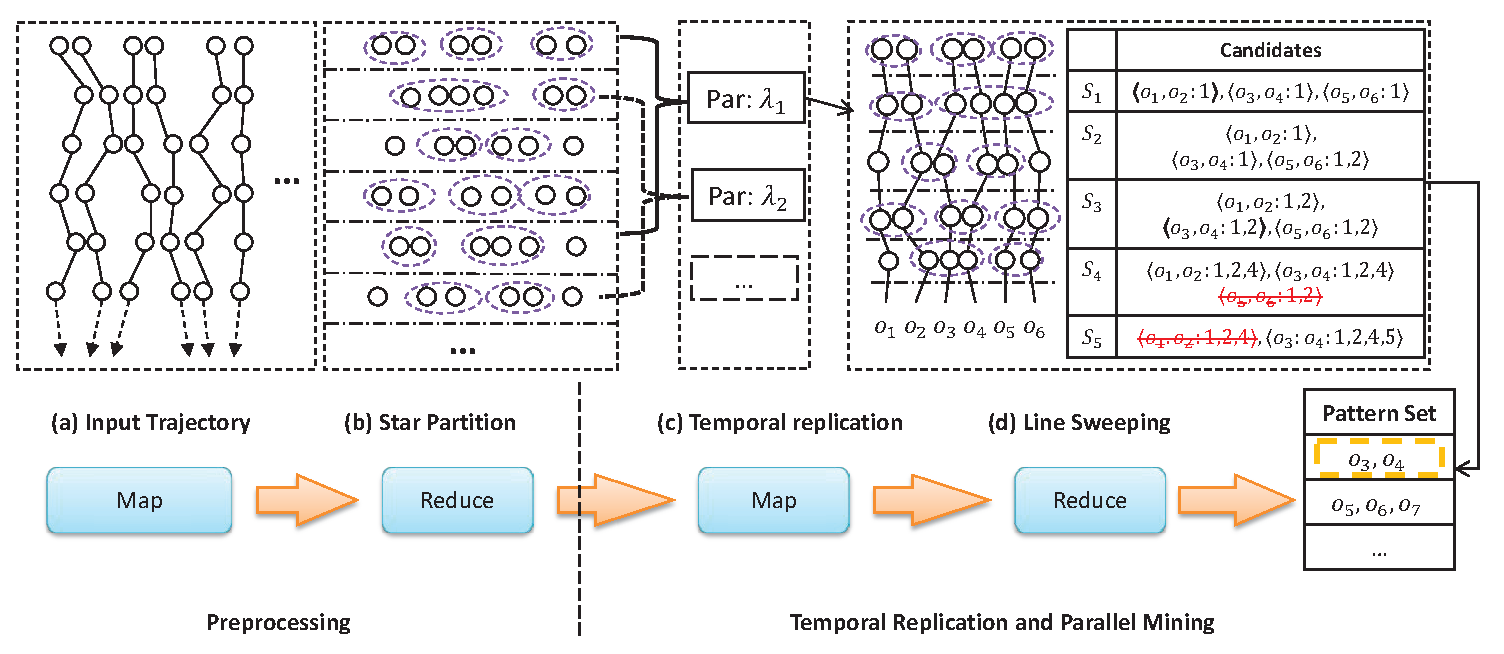
\includegraphics[width=\textwidth]{trm.eps}
\caption{Work flow of Temporal Replication and Mining. (a)(b) correspond to the first map-reduce cycle which clusters objects in each snapshot;  (c)(d) correspond to the second map-reduce cycle which uses temporal replication to mine GCMP in parallel.}
\label{fig:trm}
\end{figure*}








\emph{
Let $T$ be an arbitrary valid temporal sequence. Since $G$ equals to 1,
$T$ can be represented as $T=(t_1, t_2,...,t_m)$, where
$t_i +1 = t_{i+1}$ and $m \geq K$. Let $T' = (t_1,...,t_k)$, $T'$ is the shortest
valid temporal sequence of $T$. Note that $T'$ is fully contained
in the partition $\lambda_{t_1} = \{S_{t_1},...,S_{t_k}\}$, therefore it can be
mined in $\lambda_{t_1}$. 
Since $T$ is an arbitrary valid temporal sequence, the minimum $\eta$ is thus $K$.
}

Inspired by the observation, we generalize the relationship between
the minimum $\eta$ and temporal parameters using the following theorem:

\begin{theorem}
\label{THM:RP_ETA}
The minimum $\eta$ to ensure the completeness of the temporal replication is:
\[
   \eta = 
\begin{cases}
    (\lceil \frac{K}{L} \rceil -1)*(G-1)+2K -2, & \text{if } G \geq 2\\
    K,              & \text{if } G = 1
\end{cases}
\]
, where $K,L,G$ are the temporal parameters.
\end{theorem}

\begin{proof}
When $G = 1$, we have demonstrated $\eta=K$
in the above observation. When $G \geq 2$, we compute $\eta$ as follows:
any $T'$ can be viewed as $n$ consecutive segments with sizes $l_1,..,l_n$
and $n-1$ gaps with sizes $g_1,...,g_{n-1}$.
Since $\eta$ is the upper bond among all $T'$s, $\eta$ can be formulated 
as follows:
\begin{equation}
\eta = \max_{n,l_i,g_i} \{ \Sigma_{i=1}^{i=n} l_i + \Sigma_{i=1}^{i=n-1} g_i \}
\end{equation}
With the following constraints: (1)$\forall l_i, L \leq l_i \leq K-1$; (2)
$\forall g_i, 1 \leq g_i \leq G-1 $; (3) $\Sigma_{i=1}^{i=n} l_i \geq K$ and
(4) $\Sigma_{i=1}^{i=n-1}l_i  \leq K-1$. Constraints (1)(2)(3) due to the 
validity of $T'$ and $G\geq 2$ (4) is because $|T'|$ is minimum.
Based on (1)(3)(4), we can derive (5):  $n \in [1, \lceil \frac{K}{L} \rceil]$.
Constraints (1)-(5) form a convex polygon and $\eta$ is monotone
increasing wrt. $n, l_i, g_i$, therefore, the maximum value of $\eta$ is taken at the upper boundaries
where $g_i = G-1$, 
$\Sigma_{i=1}^{i=n-1}l_i = K-1$, $l_i = K-1$
and $n = \lceil \frac{K}{L} \rceil$. This leads to  $\eta = (\lceil \frac{K}{L} \rceil -1)*(G-1)+2K -2$.
\end{proof}

Based on the above theorem, during TRPM, every consecutive $\eta$ snapshots
form a partition. In particular, for every snapshot $S_t$, there is
a partition $\lambda_t=\{S_t,...,S_{t+\eta-1}\}$. With this partition strategy,
when discovering GCMPS in $\lambda_t$, we only need to keep the pattern candidates whose
object set are in $S_t$. This motivates to design an efficient 
\emph{line-sweep} mining (LSM) method for each partition. The intuition of LSM is 
to sequentially scan all snapshots. During scanning, a set of pattern candidates is maintained.
When all snapshots are scanned, the remaining candidates are the true patterns.
The detail of LSM is presented in Algorithm~\ref{algo:line-sweep}.
A candidate set $C$ is maintained throughout the algorithm(line~\ref{code:ls-can-set}). $C$
is initialized by inserting clusters at $S_t$ (lines~\ref{code:ls-init-start}-\ref{code:ls-init-end}).
During scanning snapshot $S_j$, candidates in $C$ are joined with clusters at $S_j$. In
the join, a candidate grows its temporal sequence while potentially reduces its object set. After the join,
false patterns are deleted (line~\ref{code:ls-remove}). 
Note that the size of $C$ is always decreasing, therefore the complexity of LSM $\lambda_t$ is $O(\eta|S_t||\overline{S}|)$,where $|\overline{S}|$ is the average snapshot size in $\lambda_t$.



\begin{algorithm}
\caption{Line Sweep Mining}
\label{algo:line-sweep}
\begin{algorithmic}[1]
\Require $\lambda_t = \{S_t, ..., S_{t+\eta-1}\}$
\State{$C \gets \{\}$} \Comment{Candidate set} \label{code:ls-can-set}
\For{$c \in S_t$} 
\label{code:ls-init-start}
\State $C$.add($\langle c, t \rangle $)
\EndFor
\label{code:ls-init-end}
\ForAll{$j \in [t+1,t+\eta-1]$}
\State $C \gets S_{j} \oplus C$ \label{code:ls-join}
	\State{remove false candidates from $C$}
	\label{code:ls-remove}
\EndFor
\State{output true candidates in $C$}
\end{algorithmic}
\end{algorithm}


%\begin{figure}[h]
%\centering
%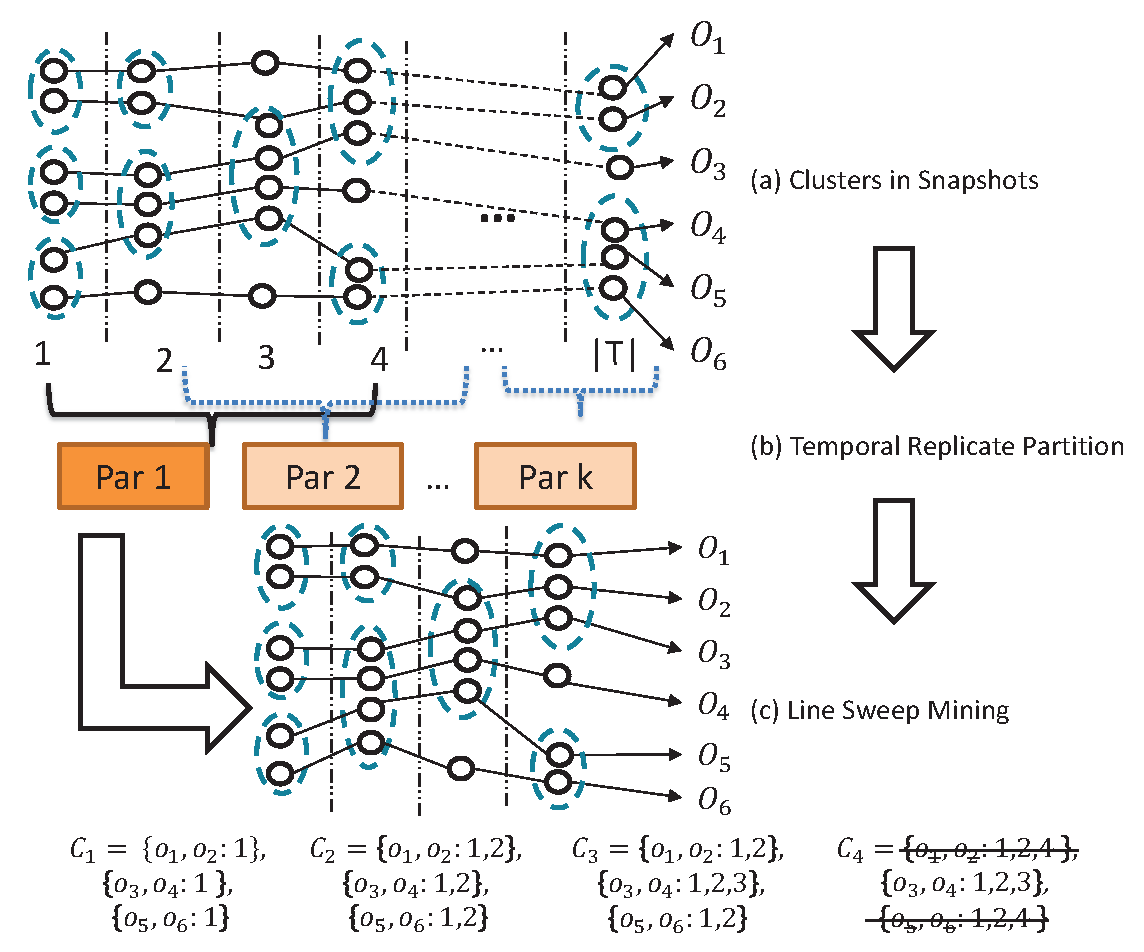
\includegraphics[width=0.5\textwidth]{trm_process.eps}
%\caption{Work flow of trajectory replication and mining}
%\label{fig:trm_process}
%\end{figure}


The complete picture of temporal replication and parallel mining is summarized in Algorithm~\ref{algo:trm_overview}. We illustrate the workflow of TRPM method using Figure~\ref{fig:trm} (c)(d) with pattern
parameters $M=2, K=3, L = 2, G=2$. By Theorem~\ref{THM:RP_ETA}, $\eta$ is calculated
as $(\lceil \frac{K}{L} \rceil-1) *(G-1)+2K - 2 = 5$. Therefore, 
in Figure~\ref{fig:trm} (c), every $5$ consecutive snapshots are combined 
into a partition in the map phase. In Figure~\ref{fig:trm} (d), a line sweep
method is illustrated for partition $\lambda_1$. Let $C_i$ be the candidate set
during sweeping snapshot $S_i$.
Initially, $C_1$ contains patterns whose object set is in snapshot $S_1$.
As line sweeps, the patterns in $C_i$ grows. At snapshot $S_4$, the candidate
$\{o_5,o_6\}$ is removed. This is because the gap between its latest timestamp (i.e., $2$)
and the next scanning timestamp (i.e., $5$) is $3$, which violates the $G$ constraint.
Next, at snapshot $S_5$, the candidate $\{o_1,o_2\}$ is removed. This is
because its local consecutive timestamps $\{4\}$ has only size $1$,
which violates the $L$ constraint.
Finally, $\{o_3,o_4\}$ is the qualified pattern and is outputted. Note that the minimum $\eta$
under this setting is $5$. If $\eta$ is chosen as $4$, the pattern $\{o_3,o_4\}$ would be excluded. 

\begin{algorithm}
\caption{Temporal Replication and Parallel Mining}
\label{algo:trm_overview}
\begin{algorithmic}[1]
\Require list of $\langle t, S_t \rangle$ pairs
\State $\eta \gets (\lceil \frac{K}{L} \rceil -1)*(G-1)+2K-2$
\State {---Map Phase---}
\label{code:trm-map-start}
\ForAll{$\langle t, S_t \rangle$}
	\ForAll{$i \in 1...{\eta-1}$}
		\State emit a $\langle \max(t-i,0), S_t \rangle$ pair
	\EndFor  
\EndFor
\label{code:trm-map-end}
\State {---Partition and Shuffle Phase---}
\label{code:trm-par-start}
\ForAll{$\langle t, S \rangle$ pair} 
\State group-by $t$, emit a $\langle t, \lambda_t\rangle$
\State where $\lambda_t = \{S_t, S_{t+1}, .. S_{t+\eta-1}\} $
\EndFor
\label{code:trm-par-end}
\State {---Reduce Phase---}
\label{code:trm-red-start}
\ForAll{$\langle t,\lambda_t \rangle$}
\State lineSweepMining($\lambda_t$)
\label{code:trm-red-end}
\EndFor
\end{algorithmic}
\end{algorithm}

\begin{figure*}[t]
\centering
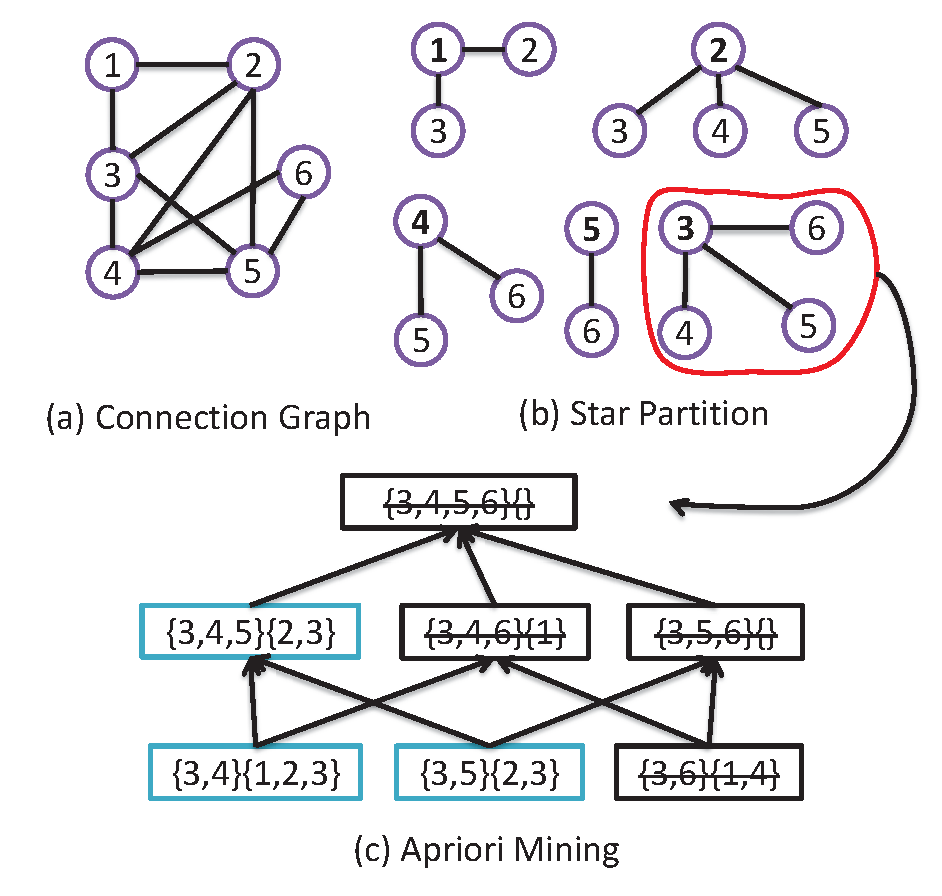
\includegraphics[width=0.9\textwidth]{spm.eps}
\caption{Star partition and mining. (a) Conceptual connection graph from Figure 1.(b) Five star partitions are generated
(c) Apriori Mining with various pruning techniques.}
\label{fig:star_partition}
\end{figure*}

\section{SPARE: Star Partitioning and Apriori Enumerator}
\label{sec:spm}
The aforementioned replicate partitioning is based on the temporal dimension which suffers from two drawbacks. First, the replication relies on $\eta$ which could be large. Second, the same valid pattern may be discovered from different partitions which results in redundant works.
%and results in groups of snapshots in each partition.
% ADD MORE DETAILS ABOUT THE LIMITATIONS HERE.
To resolve the limitations caused by the replicate partitioning, 
we propose a new Star Partitioning and ApRiori Enumerator, named SPARE, 
to replace the second cycle of map-reduce jobs in Figure~\ref{fig:trm}. 
Our new parallel mining framework is shown in Figure~\ref{fig:star_partition}. 
Its input is the set of clusters generated in each snapshot and the output 
contains all the valid GCMP patterns. In the following, we explain the two major components: 
star partitioning and apriori enumerator.


\subsection{Star Partitioning}
Let $G_t$ be a graph for snapshot $S_t$, in which each node 
is a moving object and two objects are connected if they appear 
in the same cluster. It is obvious that $G_t$ consists of a set of small cliques. 
Based on $G_t$, we define an aggregated graph $G_A$ to summarize the 
cluster relationship among all the snapshots. In $G_A$, two objects
form an edge if they are connected in any $G_t$s. Furthermore, 
we attach an inverted list for each edge, 
storing the associated timestamps in which the two objects are connected. 
An example of $G_A$, built on the trajectory database in Figure~\ref{fig:related_work}, 
is shown in Figure~\ref{fig:star_partition} (a). 
As long as two objects are clustered in any timestamp, they are connected in $G_A$. 
The object pair $(o_1,o_2)$ appears in two clusters at timestamps 
$2$ and $3$ and is thus associated with an inverted list $\{2,3\}$.


We use \emph{star} as the data structure to capture the pair relationships. 
To avoid duplication, as $G_t$ is an undirected graph and an edge may appear in multiple stars, 
we enforce a global ordering among the objects and propose a concept named \textit{directed star}.

\begin{definition}[Directed Star]
Given a vertex with global id $s$, its directed star $Sr_s$ is defined as the set of neighboring vertices with global id $t>s$. We call $s$ the star ID.
\end{definition}

With the global ordering, we can guarantee that each edge is contained in a unique star partition. Given the aggregated graph $G_A$  in Figure~\ref{fig:star_partition} (a), we enumerate all the possible directed stars in Figure~\ref{fig:star_partition} (b). These stars are emitted from mappers to different reducers. The key is the star ID and the value is the neighbors in the star as well as the associated inverted lists. 
The reducer will then call the Apriori-based algorithm to enumerate all the valid GCMP patterns.


Before we introduce the Apriori enumerator, we are interested to 
examine the issue of global ordering on the moving objects.
This is because assigning different IDs to the objects will result in 
different star partitioning results, which will eventually affect the workload 
balance among the map-reduce jobs. The job incurring performance bottleneck is often known as \emph{straggler}~\cite{kwon2012skewtune,xin2013shark,coppa2015data}. In the context of star partitioning, a straggler refers to the job assigned with the maximum star partition. We use $\Gamma$ to denote the size of a partition and $\Gamma$ is set to the number of edges in a directed star\footnote{A star is essentially a tree structure and the number of nodes equals the number of edges minus one.}. It is straightforward that a star partitioning with small $\Gamma$ is preferred. For example, Figure~\ref{fig:star-alt} gives two star partitioning results under 
different vertex ordering on the same graph. The top one has $\Gamma = 5$ while the bottom one has $\Gamma = 3$. Obviously, the bottom one with smaller $\Gamma$ is much more balanced.


%An important concern in design parallel algorithms is the distribution of work loads.  
%Traditionally, the quality of a partition strategy 
%is measured based on two aspects: (1) the number of result partition, which
%affects the maximum parallelism
%(2) the size balance of partitions, which affects the finishing
%time of a job. Unlike TRM where each partition
%contains equal-sized snapshots, the size distribution 
%of stars in SPM remains unknown.
%Nevertheless, we notice that, in SPM, the total sizes of 
%stars are invariant. Therefore, the quality of a star partition
%can be formalized as the \emph{skewness}, which is the maximum star size
%among all stars. Smaller \emph{skewness} naturally results in more partitions
%and less imbalance.
%}

\begin{figure}[h]
\centering
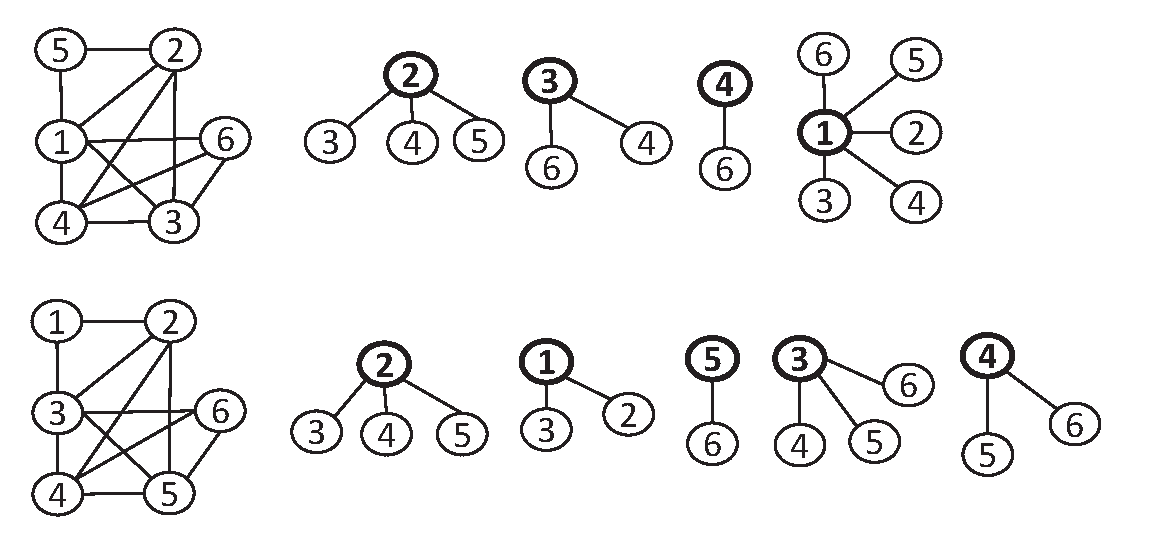
\includegraphics[width=0.5\textwidth]{star-alt.eps}
\caption{Examples of star partitioning with different vertex ordering.}
\label{fig:star-alt}
\end{figure}


%To determine the optimal vertex orders with the objective of minimizing $\Gamma$, 
%we can use a linear algebra model as follows:  
%Let $G_A$ be an aggregate graph, with a $n \times n$ adjacent matrix $J$.
%A vertex order is in fact a permutation of $J$. Therefore,
%the adjacent matrices of any reordered graphs can be represented as $PJP^T$
%where $P \in \mathbb{P}$ is a 
%\emph{permutation matrix}~\footnote{an identity matrix with rows shuffled} with dimension $n$.
%Since in star partition, we assign each edge $e(i,j)$ in $G_A$ to the lower vertex, 
%then the matrix $B=\triu(PJP^T)$~\footnote{\text{triu} is the upper triangle part of a matrix}
%represents the assignment matrix wrt. $P$ (i.e., $b_{i,j} = 1$ if vertex $j$ is in star $Sr_i$).
%Let vector $\vec{b}$ be the \textit{one}\footnote{every element in $\vec{b}$ is $1$} 
%vector of size $n$. Let $\vec{c} = B\vec{b}$, then each $c_i$ 
%denotes the number of edges in star $Sr_i$. Thus, $\Gamma$ can be represented
%as the infinity norm of $B\vec{b}$. Let $\Gamma^*$ be the minimum $\Gamma$ among all vertex orders. 
%$\Gamma^*$ can then be formulated as follows:
%\begin{equation}
%\Gamma^* = \min_{P \in \mathbb{P}}{||B\vec{b}||_\infty} \text{ ,where } ||B\vec{b}||_\infty = \max_{1\leq j \leq n}(c_j)
%\end{equation}

Although it is very challenging to find the optimal vertex id ordering from the $n!$ possibilities, we observe that a random order can actually achieve satisfactory performance based on the following theorem.



\begin{theorem}
\label{THM:SPM_LB}
Let $\Gamma^*$ be the value derived from the optimal vertex ordering and  $\Gamma$ be value derived from a random vertex ordering. With probability $1-1/n$, we have $\Gamma = \Gamma^* + O(\sqrt{n \log n})$.
\end{theorem}
\begin{proof}
In Appendix XXX.
\end{proof}
If $G_A$ is a dense graph, we can get a tighter bound for $(\Gamma - \Gamma^*)$.
\begin{theorem}
\label{THM:SPM_LB_INC}
Let $d$ be the average degree in $G_A$. If $d\geq \sqrt{12\log n}$, with
high probability $1-1/n$, $\Gamma = \Gamma^* + O(\sqrt{d\log n})$.
\end{theorem}
\begin{proof}
In Appendix XXXX.
\end{proof}
Hence, we can simply use object id to determine the vertex ordering in our implementation.


%
%Even though the TRM algorithm works in a parallel way, it requires to replicate the data $\eta$ times. 
%When $\eta$ is small, TRM perform good parallelism. However, wh
%
%When handling \emph{swarm}, \emph{group} and \emph{platoon} patterns, $\eta$ has to be set to $|\mathbb{T}|$ to guarantee correctness, resulting in very expensive data replication overhead. 
%%Handling those cases are equivalent to replicate the entire snapshots to each partition, 
%%which surrenders the benefit of parallelism.
\eat{
Although TRPM works in a parallel way, we observe two inefficiencies. First, the
performance of TRPM largely relies on $\eta$ which further depends on pattern parameters.
When $\eta$ is large, the shuffle and reduce cost of TRPM is high. Second, 
the parallel execution of line sweep algorithm may discover the same pattern from
multiple partitions, which introduces redundant work. To resolve the two limitations,
we design a novel \emph{Star Partition and Mining} algorithm.
}
%After computing the star, each partition is applied with a reduce task. 
%Indeed, a star $Sr_s$ can be viewed as a subset of original trajectories. 
%This is done by treating each vertex in $Sr_s$ as an object. 
%The time sequence of $s$ is the union of all edges in $Sr_s$. 
%And the time sequence of $v \neq s$ is the edge $(s,v)$. Therefore, we
%are able to mine stars from the similar trajectory concepts.

\subsection{Apriori Enumerator}
Intuitively, given a GCMP pattern with an object set $\{o_1,o_2,\ldots,o_m\}$, 
all the pairs of $(o_i,o_j)$ with $1\leq i<j\leq m$ must 
be connected in the associated temporal graphs $\{G_t\}$. This inspires us to leverage the classic Apriori algorithm to enumerate all the valid GCMP patterns starting from pairs of objects. However, we observe that the monotonicity property does not hold between an object set and its supersets.

\begin{example}
In this example, we show that if an object set is not a valid pattern, we cannot prune all its super sets.
Consider two candidates $P_1=\{o_1,o_2:1,2,3,6\}$ and $P_2=\{o_1,o_3:1,2,3,7\}$. 
Let $L=2,K=3$ and $G=2$. Both candidates are not valid patterns because the constraint on $L$ is not satisfied. 
However, when considering their object superset $\{o_1,o_2,o_3\}$, we can infer that their co-clustering timestamps are in $(1,2,3)$. This is a valid pattern conforming to the constraints of $L,K,G$. Thus, we need a new type of monotonicity to facilitate pruning.
\end{example}   


\subsubsection{Monotonicity}
To ensure the monotonicity, we first introduce a procedure named \textit{star simplification}, to reduce the number of edges as well as unnecessary timestamps in the inverted lists. For instance, if the size of the inverted list for an edge $e$ is smaller than $K$, then the edge can be safely removed because the number of timestamps in which its supersets are clustered must also be smaller than $K$. To generalize the idea, we propose three concepts named \textit{maximal $G$-connected subsequence}, \emph{decomposable sequence} and \emph{sequence simplification}.

\begin{definition}[Maximal $G$-connected Subsequence]
A sequence $T'$ is said to be a maximal $G$-connected subsequence of $T$ if (1) $T'$ is the subsequence of $T$, i.e., $\exists i\leq j, T' = T(i,\ldots,j)$ , (2) $T'$ is $G$-connected, and (3) there exists no other subsequence $T''$ of $T$ such that $T'$ is the subsequence of $T''$ and $T''$ is G-connected.
\end{definition}
%Hence, our idea is to examine the validity of object pairs. If $(o_i,o_j)$ itself is not a valid GCMP pattern, then all the supersets containing $(o_i,o_j)$ can be pruned. For instance, $(XXX,XXX)$ are not connected in Figure~\ref{} and all its supersets can be pruned.

\begin{example}
Suppose $G=2$ and consider two sequences $T_1=(1,2,4,5,6,9,10,11,13)$ and $T_2=(1,2,4,5,6,8,9)$. $T_1$ has two maximal $2$-connected subsequences:$T_1^A=(1,2,4,5,6)$ and $T_1^B=(9,10,11,13)$. This is because the gap between $T_1^A$ and $T_1^B$ is $3$ and it is impossible for the timestamps from  $T_1^A$ and $T_1^B$ to form a new subsequence with $G\leq 2$. Since $T_2$ is $2$-connected, $T_2$ has only one maximal $2$-connected subsequence which is
itself. 
\end{example}

The maximal $G$-connected subsequence has the following two properties:
\begin{lemma}\label{lemma:union-property}
Suppose $\{T_1,T_2,\ldots,T_m\}$ is the set of all maximal $G$-connected subsequences of $T$, we have (1) $T_i\cap T_j=\emptyset$ for $i\neq j$ and (2) $T_1\cup T_2\cup\ldots\cup T_m=T$.
\end{lemma}
\begin{proof}
We assume $T_i\cap T_j\neq \emptyset$. Let $T_i=(T_i[1], T_i[2],\ldots,T_i[p])$ and $T_j= (T_j[1], T_j[2],\ldots,T_j[n])$. Suppose $T[x]$ is a timestamp occurring in both $T_i$ and $T_j$. Let $T[y]=\min\{T_i[1],T_j[1]\}$, i.e., the minimum timestamp of $T_i[1]$ and $T_j[1]$ occurs at the $y$-th position of sequence $T$. Similarly, we assume $T[z]=\max\{T_i[p], T_j[n]\}$. Apparently, the two subsequences $T[y:x]$ and $T[x:z]$ are $G$-connected because $T_i$ and $T_j$ are both $G$-connected. Then, sequence $(T_y,\ldots,T_x,\ldots,T_z)$, the superset of $T_i$ and $T_j$, is also $G$-connected. This contradicts with the assumptions that $T_i$ and $T_j$ are maximal $G$-connected subsequences. 




To prove (2), we assume $\cup_i T_i$ does not cover all the timestamps in $T$. Then, we can find a subsequence $T'=T[x:x+t]$ such that $T[x-1]\in T_a$ $(1\leq a\leq m)$, $T[x+t+1]\in T_b$ $(1\leq b\leq m)$ and all the timestamps in $T'$ is not included in any $T_i$. Let $g'=\min\{T[x]-T[x-1], T[x+t+1]-T[x+t]\}$. If $g'\leq G$, then it is easy to infer that $T_a$ or $T_b$ is not a maximal $G$-connected subsequence because we can combine it with $T[x]$ or $T[x+t]$  to a form superset which is also $G$-connected. If $g'>G$, $T'$ itself is a maximal $G$-connected subsequence which is missed in $\cup T_i$. Both cases lead to contradiction.
\end{proof}




\begin{lemma}\label{lemma:subset-property}
If $T_1$ is a subset of $T_2$, then for any maximal $G$-connected subsequence $T_1'$ of $T_1$, we can find a maximal $G$-connected subsequence $T_2'$ of $T_2$ such that $T_1'$ is a subset of $T_2'$.
\end{lemma}
\begin{proof}
Since $T_1' \subseteq T_1 \subseteq T_2 $, we know $T_1'$ is a $G$-connected subsequence of $T_2$. Based on Lemma~\ref{lemma:union-property}, we can find a maximal $G$-connected subsequence of $T_2$, denoted by $T_2'$, such that $T_1'\cap T_2'\neq \emptyset$. If there exists a timestamp $T_1'[x]$ such that $T_1'[x]\notin T_2'$, similar to the proof of case (1) in Lemma~\ref{lemma:union-property}, we can obtain a contradiction. Thus, all the timestamps in $T_1'$ must occur in $T_2'$.
\end{proof}

\begin{definition}[Decomposable Sequence]
$T$ is decomposable if for any of its maximal $G$-connected subsequence $T'$, we have (1) $T'$ is $L$-consecutive; and (2) $|T'|\geq K$.
\end{definition}

\begin{example}
Let $L = 2, K = 4$ and we follow the above example. $T_1$ is not a decomposable sequence
because one of its maximal $2$-connected subsequence (i.e., $T_1^B$) is not $2$-consecutive.
In contrast, $T_2$ is a decomposable sequence because the sequence itself is the maximal $2$-connected subsequence, which is also $2$-consecutive and with size no smaller than than $4$.
\end{example}


%Not that, although $T_1$ is not a candidate sequence, it can be simplified
%to a candidate sequence (i.e, $T_2$). Generally, for any time sequence $T$, 
%if it does not contain a \emph{candidate sequence}, then it cannot contribute
%to any valid patterns. In fact, only the candidate sequence inside $T$ affects
%the final patterns. Therefore, we may use the candidate sequence to simplify edges in 
%a star. During the simplification, if an edge results in a candidate
%sequence of size zero, then it is removed from the star. Otherwise,
%the simplified edge is kept. By so doing, the size of the new star
%is much smaller.

\begin{definition}[Sequence Simplification]
Given a sequence $T$, the simplification procedure $\mathtt{sim}(T) =  g_{G,K} \cdot f_L(T) $ can be seen as a composite function with two steps: 
\begin{enumerate}
\item $f$-step: remove segments of $T$ that are not $L$-consecutive;
\item $g$-step: among the maximal $G$-connected subsequences of $f_L(T)$, remove those with size smaller than $K$.
\end{enumerate}
\end{definition}


\begin{example}
Take $T=(1,2,4,5,6,9,10,11,13)$ as an example for sequence simplification. 
Let $L = 2, K = 4$ and $G = 2$. In the $f$-step, $T$ is reduced to $f_2(T)=(1,2,4,5,6,9,10,11)$. 
The segment $(13)$ is removed due to the constraint of $L=2$. 
$f_2(T)$ has two maximal $2$-consecutive subsequences: $(1,2,4,5,6)$ and $(9,10,11)$. 
Since $K=4$, we will remove $(9,10,11)$ in the $g$-step. Finally, the output is $\mathtt{sim}(T)=(1,2,4,5,6)$.
\end{example}

It is possible that the simplified sequence $\mathtt{sim}(T)=\emptyset$. For example, Let $T=(1,2,5,6)$ 
and $L=3$. All the segments will be removed in the $f$-step and the output is $\emptyset$.
We define $\emptyset$ to be not decomposable. 
%Based on the above definitions, we can define our monotonicity to facilitate the pruning in the Apriori algorithm.
We provide an important property of the sequence simplification process as follows:
\begin{lemma}\label{lemma:decom-sim}
If sequence $T$ is a superset of any decomposable sequence, then $\mathtt{sim}(T) \neq \emptyset$.
\end{lemma}
\begin{proof}
It is obvious that $\mathtt{sim}(T)$ is a one-to-one function. Given an input sequence T, there is a unique  $\mathtt{sim}(T)$. Let $T_p$ be a decomposable subset of $T$ and we prove the lemma by showing that $\mathtt{sim}(T)$ is a superset of $T_p$.

Suppose $T_p$ can be decomposed into a set of maximal $G$-connected
subsequences $T_p^1, \ldots, T_p^m$ ($m \geq 1$). Since $T_p$ is a subset of $T$, all the $T_p^i$ are also subsets of $T$. By definition, each $T_p^i$ is $L$-consecutive. Thus, in the $f$-step of $\mathtt{sim}(T)$, none of $T_p^i$ will be removed. In the $g$-step, based on Lemma~\ref{lemma:subset-property}, we know that each $T_p^i$ has a superset in the maximal $G$-connected subsequences of $f_L(T)$. Since $|T_p^i|\geq K$, none of $T_p^i$ will be removed in the $g$-step. Therefore, all the $T_p^i$ will be retained after the simplification process and $\mathtt{sim}(T) \neq \emptyset$.
\end{proof}



\eat{
Nevertheless, if there exists a $T^\#$ of $T$, then $T^\#$ is unique
as stated in the following theorem:
\begin{theorem}
For any sequence $T$, if $T$'s simplified sequence is not empty, then
there exists a unique $T^\#$ wrt $T$.
\end{theorem}
\begin{proof}
We prove by contradiction. Suppose there are two simplified sequences $T_A^\#$ and $T_B^\#$ of the same $T$. We prove that, unless $T_B^\# \equiv T_A^\#$, $T_A^\#$ can always be enlarged, which leads to a contradiction. For simplicity, we use $\overline{ab}$ to denote the segment of a sequence from timestamp $a$ to timestamp $b$.
Consider the timestamps $T_C=T_B^\# - T_A^\#$. If $T_C = \emptyset$, then $T_A^\# \equiv T_B^\#$ naturally.

Next, since $T_C \not \equiv \emptyset$, W.L.O.G, let the first timestamp in $T_A^\#$ be greater than the first timestamp $T_B^\#$. Consider the general setting: $\overline{ab}$ is the first candidate sequence in $T_A^\#$;  $\overline{ef}$
is a consecutive sequence in $T_C$ and $f < a$; $\overline{cd}$ is the next candidate sequence of $\overline{ef}$ in $T_B^\#$; $\overline{gh}$ is the previous candidate sequence of $\overline{ef}$ in $T_B^\#$; Categorize on the gaps between $\overline{ef}$ and  $\overline{cd}$, $\overline{gh}$,
there are four cases to be considered. 
We demonstrate the cases in Figure~\ref{fig:proof_thm_3}:
\begin{figure}[h]
\centering
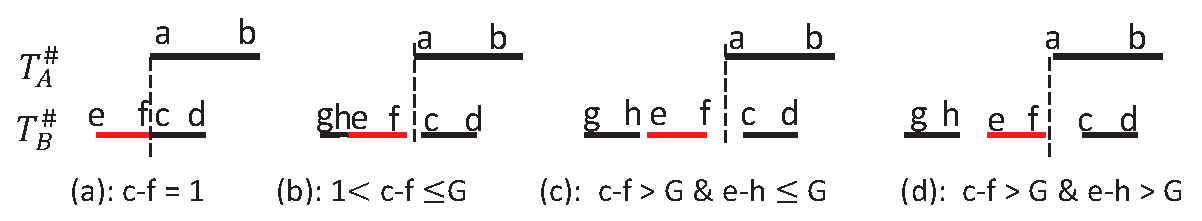
\includegraphics[width=0.46\textwidth]{thm3proof.eps}
\caption{Proof of theorem 3 with the four cases.}
\label{fig:proof_thm_3}
\end{figure}
\begin{itemize}
\item Case (a): $c-f = 1$, that is $\overline{ef}$ is part of a longer consecutive segment $\overline{ed}$. Since timestamp $c$ is in $T_A^\#$, $T_A^\#$ can be safely enlarged by increasing $\overline{ab}$ to $\overline{eb}$.
\item Case (b): $G \geq c-f> 1$. In this case, since $c\geq a$, then $a-f \leq G$. Further, since $\overline{ed}$ is not 
consecutive, $\overline{ef}$ must belongs to a larger consecutive segment $\overline{gf}$ with size no less than $L$. Therefore, adding $\overline{gf}$ to $\overline{ab}$ makes $\overline{gb}$ still a candidate sequence.
\item Case (c): $c-f > G$ and $e-h \leq G$. In this case, $\overline{ef}$ belongs to a candidate sequence $\overline{gf}$ in $T_B^\#$.  Since $\overline{gf}$ has no intersection with $\overline{ab}$, then adding $\overline{gf}$ to $T_A^\#$ is valid.
\item Case (d): $c-f > G$ and $ e- h > G$. In this case,  $\overline{ef}$ has to be a candidate sequence. Since $\overline{ef}$ has no intersection with $\overline{ab}$, adding $\overline{ef}$ to $\overline{ab}$ is valid.
\end{itemize}
In all cases, $T_A^\#$ can be enlarged, which contradicts with the assumption $T_A^\#$ is the simplified sequence. This completes the proof.
\end{proof}
}



\eat{
Next, we design an efficient simplification process with linear complexity.
It takes two rounds scan of $T$ as shown in Algorithm~\ref{algo:simp_prune}. 
In the first round, the consecutive portions of $T$ with size less than $L$ are removed.
In the second round, the maximal $G$-connected sequences of size less than $K$ are removed. 

\begin{algorithm}
\caption{Edge Simplification}
\label{algo:simp_prune}
\begin{algorithmic}[1]
\Require $T$
\State{---$L$ Phase---}
\State $c \gets 0$
\For {$i \in (0,...,|T|)$}
	\If{$T[i] - T[i-1] > 1$} 
		\If{$i - c < L$} 
			\State $T$ remove $[c:i)$
		\EndIf
		\State $c \gets i$
	\EndIf
\EndFor
\State{---$G$-$K$ Phase---}
\State $s\gets 1$, $c\gets 0$
\For{$i \in (0: |T|)$}
	\If{$T[i] - T[i-1] > G$}
		\If{$s < K$}   
			\State $T$ remove $[c:i)$
		\EndIf
		\State {$c \gets i$, $s \gets 1$}
	\Else
		\State $s++$
	\EndIf
\EndFor
\end{algorithmic}
\end{algorithm}
}

With Lemma~\ref{lemma:decom-sim}, we are ready to define the \emph{monotonicity} based on the simplified
sequences to facilitate the pruning in the Apriori algorithm. 

\begin{theorem}[Monotonicity]\label{THM:SPARE_MONO}
Given a candidate pattern $P=\{O:T\}$, if $\mathtt{sim}(P.T)=\emptyset$, then any pattern candidate $P'$ with $P.O \subseteq P'.O$ can be pruned.
\end{theorem}

\begin{proof}
We prove by contradiction. Suppose there exists a valid pattern $P_2$ such that $P_2.O \supseteq P.O$. It is obvious that $P_2.T \subseteq P.T$. Based on the Definition 2, the following conditions hold: (1) $P_2.T$ is $G$-connected. (2) $|P_2.T| \geq K$ and (3) $P_2.T$ is $L$-consecutive. Note that the entire $P_2.T$ is $G$-connected. Thus, $P_2.T$ itself is the only maximal $G$-connected subsequence. Based on conditions (1),(2),(3) and Definition 6, $P_2.T$ is decomposable. Then, based on Lemma~\ref{lemma:decom-sim}, we know $\mathtt{sim}(T)\neq \emptyset$ because $P_2.T \subseteq P.T$ and $P_2.T$ is decomposable. This leads to a contradiction with $\mathtt{sim}(P.T)=\emptyset$.
\end{proof}

%IN THE PROOF, YOU NEED TO SHOW 1) $P$ IS NOT VALID 2) ALL THE SUPERSETS OF $P.O$ ARE NOT VALID.












\subsubsection{Apriori Enumeration}
We design an Apriori enumeration method to efficiently discover all the valid patterns in a star partition. The principle of Apriori algorithm is to construct a lattice structure and enumerate all the possible candidate sets in a bottom-up manner. Its merit lies in the monotonic property such that if a candidate set is not valid, then all its supersets can be pruned. Thus, it works well in practice in spite of the exponential search space.

Our customized Apriori Enumerator is presented in Algorithm~\ref{algo:apriori_mining}. Initially, the edges (pairs of objects) in the star constitute the bottom level (Lines~\ref{code:init-start}-\ref{code:init-end}) and unqualified candidates are excluded (Line~\ref{code:simp1}). A indicator \emph{level} is used to control the object size of the current candidates. During each iteration (Lines~\ref{code:level-start}-\ref{code:level-ends}), only candidates with object size equals to \emph{level} are generated (Line~\ref{code:join-start}). When two candidate sets $c_1$ and $c_2$ are joined, the new candidate becomes $c'=\langle c_1.O \cup c_2.O, c_1.T\cap c_2.T\rangle$ (Lines~\ref{code:join}). To check the validity of the candidate, we calculate $\mathtt{sim}(c'.T)$. If its simplified sequence is empty, $c'$ is excluded from the next level (Line~\ref{code:simp2}). This ensures that
then all the candidates with $P.O\supseteq c'.O$ are excluded. If a candidate cannot generate any new candidates, then it is directly outputted (Lines~\ref{code:output1-start}-\ref{code:output1-end}).
To further improve the performance, we adopt the idea of \textit{forward closure}~\cite{wang2003closet+,pei2000closet} and  aggressively check if the union of all the current candidates form a valid pattern (Lines~\ref{code:fc-checking-start}-\ref{code:fc-checking-end}). If yes, we can early terminate the algorithm and output the results.

\begin{algorithm}
\caption{Apriori Enumerator}
\label{algo:apriori_mining}
\begin{algorithmic}[1]
\Require{$Sr_s$}
\State {$C \leftarrow \emptyset$}
\ForAll{edges $c=\langle o_i\cup o_j, T_{o_i}\cap T_{o_j}\rangle$ in $Sr_s$} \label{code:init-start}
\If {$\mathtt{sim}(T_{o_i}\cap T_{o_j})\neq \emptyset$}
\State {$C\leftarrow C\cup \{c\}$} \label{code:simp1}
%\ElsIf{$c$ is a valid pattern}
%\State{output $c$}
\EndIf 
\EndFor\label{code:init-end}
\State $\mathrm{level} \gets 2$ \label{code:level}
\While{$C\neq \emptyset$} \label{code:level-start}
	\ForAll{$c_1 \in C$}
		\ForAll{$c_2 \in C$ and $|c_2.O \cup c_2.O| = \mathrm{level}$}\label{code:join-start}	
			\State {$c' \gets \langle c_1.O \cup c_2.O:(c_1.T \cap c_2.T )\rangle$} \label{code:join}			
			\If{ $\mathtt{sim}(c'.T)\neq \emptyset$} \label{code:simp2}
					\State {$C'\leftarrow C'\cup \{c'\}$}
			\EndIf			
		\EndFor\label{code:join-end}
		\If {no $c'$ is added to $C'$} \label{code:output1-start}
			\If{$c_1$ is a valid pattern}
				\State output $c_1$
			\EndIf
		\EndIf \label{code:output1-end}
	\EndFor
%	
%		\ForAll{pairs $c_1\in C$, $c_2\in C$ and $c_1\neq c_2$} \label{code:join-start}
%				\State {$c' \gets \langle c_1.O \cup c_2.O:(c_1.T \cap c_2.T )\rangle$} \label{code:join}
%				\If{ $\mathtt{sim}(c_1.T \cap c_2.T )\neq \emptyset$}
%					\State {$C'\leftarrow C'\cup \{c'\}$}
%					\ElsIf{$c'$ is a valid pattern}
%						\State{output $c'$}
%				\EndIf
%		\EndFor	\label{code:join-ends}
	\State $O_u \gets $ union of $c.O$ in $C$	\label{code:fc-checking-start}
	\State $T_u \gets $ intersection of $c.T$ in $C$	
	\If {$\langle O_u, T_u\rangle$ is a valid pattern}
		\State{output $\langle O_u, T_u\rangle$} \label{code:fc-checking}
		\State break;
	\EndIf \label{code:fc-checking-end}
	\State {$C\leftarrow C';C'\leftarrow \emptyset; \mathrm{level} \gets \mathrm{level}+1$}	
\EndWhile\label{code:level-ends}
\State output $C$ \label{code:output2-end}
\end{algorithmic}
\end{algorithm}



\begin{example}
As shown in Figure~\ref{fig:star_partition}(c), in the bottom level of the lattice structure, candidate $\{3,6:3\}$ is pruned because its simplified sequence is empty. Thus, all the object sets containing $\{3,6\}$ can be pruned. The remaining two candidates (i.e., $\{3,4:1,2,3\}$ and $\{3,5:2,3\}$)  derive a new  $\{3,4,5:2,3\}$ which is valid. By the forward closure checking, the algorithm can terminate and output $\{3,4,5:2,3\}$ as the final closed pattern.
\end{example}




\subsection{Put It Together}
We summarize the workflow of SPARE in Figure~\ref{fig:star_partition} as follows. After the parallel clustering in each snapshot, for ease of presentation, we used an aggregated graph $G_A$ to capture the clustering relationship. However, in the implementation of the map phrase, there is no need to create $G_A$ in advance.  Instead, we simply need to emit the edges within a star partition to the same reducer.  Each reducer is an Apriori Enumerator. When receiving a star $Sr_i$, the reducer creates initial candidate patterns. Specifically, for each $o \in Sr_i$, a candidate pattern $\{o,i: e(o,i)\}$ is created. Then it enumerates all the valid patterns from the candidate patterns. The pseudocode of SPARE is presented in Algorithm~\ref{algo:spm_overview}. 

\begin{algorithm}
\caption{Star Partition and ApRiori Enumerator}
\label{algo:spm_overview}
\begin{algorithmic}[1]
\Require list of $\langle t, S_t \rangle$ pairs
\State {---Map phase---}
\label{code:spm-map-start}
\ForAll{$C \in S_t$}
	\ForAll {$o_1 \in C,  o_2 \in C, o_1 < o_2$}
	\State emit a $\langle o_1, o_2, \{t\}\rangle$ triplet~\label{code:spm-edge-direct}
	\EndFor
\EndFor
\label{code:spm-map-end}

\State {---Partition and Shuffle phase---}
\label{code:spm-shuffle-start}
\ForAll{$\langle o_1, o_2, \{t\}\rangle$ triplets} 
	\State group-by $o_1$, emit $\langle o_1, Sr_{o_1} \rangle$ 
	%\State group-by $o_2$, emit $\langle o_2, Sr_{o_2} \rangle$
\EndFor
\label{code:spm-shuffle-end}

\State {---Reduce phase---}
\label{code:spm-reduce-start}
\ForAll{$\langle o, Sr_{o} \rangle$}
\State AprioriEnumerator($Sr_o$)
\EndFor
\label{code:spm-reduce-end}

\end{algorithmic}
\end{algorithm}

Compared with TPMP, the SPARE framework does not rely on snapshot replication to guarantee correctness. In addition, we can show that the patterns derived from a star partition are unique and there would not be duplicate patterns mined from different star partitions.
\begin{theorem}[Pattern Uniqueness]
\label{LEM:SPM_CORRECT}
Let $Sr_i$ and $Sr_j$ ($i\neq j$) be two star partitions. Let $P_i$ (resp. $P_j$) be 
the patterns discovered from $Sr_i$ (resp. $Sr_j$). 
Then, $\forall p_i \in P_i, \forall p_j \in P_j$, we have $p_i.O \neq p_j.O$.
\end{theorem}
\begin{proof}
We prove by contradiction. Suppose there exist $p_i \in P_i$ and $p_j \in P_j$ with the same object set. Note that the center vertex of the star is associated with the minimum id. Let $o_i$ and $o_j$ be the center vertices of the two partitions and we have $o_i=o_j$. However, $P_i$ and $P_j$ are different stars, meaning their center vertices are different (i.e., $o_i\neq o_j$), leading to a contradiction. 
\end{proof}

Theorem~\ref{LEM:SPM_CORRECT} implies that no mining efforts are wasted in discovering redundant patterns  
%that no replication is required 
in the SPARE framework, which is superior to the TRPM baseline. Finally, we prove the correctness of the SPARE framework.
\begin{theorem}
\label{THM:SPM_CORRECT}
The SPARE framework guarantees completeness and soundness.
\end{theorem}
\begin{proof}
See Appendix XXXX.
\end{proof}

\section{Experimental Study}
\label{sec:exp}
In this section, we evaluate the efficiency and scalability of our proposed parallel GCMP detectors on real trajectory datasets. All the experiments are carried out in a cluster with $12$ nodes, each equipped with four quad-core $2.2$GHz Intel processors, $32$GB memory and gigabit Ethernet. 

\textbf{Environment Setup}: We use Yarn\footnote{\url{http://hadoop.apache.org/docs/current/hadoop-yarn/hadoop-yarn-site/YARN.html}} to manage our cluster. We pick one machine as Yarn's master node, and for each of the remaining machines, we reserve one core and $2$GB memory for Yarn processes. We deploy our GCMP detector on Apache Spark 1.5.2~\cite{zaharia2012resilient} with the remaining $11$ nodes as the computing nodes.
To fully utilize the computing resources, we configure each node to run five executors, each taking three cores and $5$GB memory. In Spark, one of the $55$ executors is taken as the Application Master for coordination, therefore our setting results in $54$ executors. \revised{We set the number of partitions to be $486$ to fully utilize the parallelism provided by the multi-threading of every core.}
All our implementations as well as cluster setups are open-sourced in Github\footnote{\url{https://github.com/fanqi1909/TrajectoryMining/}}.

\textbf{Datasets}: We use three real trajectory datasets in different application scenarios:
\begin{itemize}
\item{Shopping}\footnote{\url{http://www.irc.atr.jp/crest2010_HRI/ATC_dataset/}}: The dataset contains
  trajectories of visitors in the ATC shopping center in Osaka. To better capture the indoor activities, the visitor locations are sampled every half second, resulting in $13,183$ long trajectories. 
\item{GeoLife}~\footnote{\url{http://research.microsoft.com/en-us/projects/geolife/}}: The dataset essentially keeps all the travel records of 182 users for a period
of over three years, including multiple kinds of transportation modes (walking, driving and taking public
transportation). For each user, the GPS information is collected periodically and 91 percent of the trajectories
are sampled every 1 to 5 seconds.
\item{Taxi}~\footnote{Taxi is our proprietary dataset}: The dataset tracks the trajectories of $15,054$ taxies in Singapore. For each taxi, the GPS information are continually collected for one entire month with the sampling rate around 30 seconds.
\end{itemize}


\textbf{Preprocessing}: We replace timestamps with global sequences (starting from $1$) for each dataset. 
We set a fixed sampling rate for each dataset (i.e., GeoLife = 5 seconds, Shopping=0.5 seconds, Taxi = 30 seconds)
and use linear interpolation to fill missing values.
%For each dataset, we set a fixed sampling rate (CLEARLY STATE THE SAMPLING RATE FOR EACH DATASET) and use linear interpolation to fill missing values. 
%Finally, we obtain a set of trajectories with equal length. 
%Finally, we obtain a set of dense trajectories with equal length. 
For the clustering method, we use DBSCAN~\cite{ester1996density} and customize its two parameters $\epsilon$ (proximity threshold) and $minPt$ (the minimum number of points required to form a dense region). We set $\epsilon=5$, $minPt=10$ for GeoLife and Shopping datasets; and $\epsilon=20$, $minPt=10$ for Taxi dataset. Note that other clustering methods or settings can also be applied. 
%The clustered snapshots are stored in HDFS as $\langle t, S_t \rangle$ pair, where $t$ is the timestamp, $S_t$ contains the clusters at snapshot $t$. 
After preprocessing, the statistics of the three datasets are listed in Table~\ref{exp:dataset}. 

\begin{table} [h]
\center
\small
\begin{tabular}{|l|l|l|l|}
\hline
 \textbf{Attributes}& \textbf{Shopping} &  \textbf{GeoLife} &  \textbf{SingTaxi} \\ 
\hline 
\# objects  & 13,183 & 18,670 & 15,054\\ 
\hline
%\# average ts & 3,114  & 2,924 & 19,667 \\ 
%\hline
\# data points  & 41,052,242 & 54,594,696 & 296,075,837\\ 
\hline
\# snapshots  & 16,931 & 10,699 & 44,364\\ 
\hline
\# clusters  & 211,403  & 206,704& 536,804\\
\hline
avg. cluster size  & 171 & 223 & 484\\
\hline
\end{tabular}
\caption{Statistics of datasets.}
\label{exp:dataset}
\end{table}

\textbf{Parameters}: To systematically study the performance of
our algorithms, we conduct experiments on various parameter settings. The parameters to be evaluated are listed in Table~\ref{tbl:parameters}, with default settings in bold. 
\begin{table}[h]
\small
\begin{tabular}{c|l|l}
\hline 
\textbf{Variables} & \textbf{Meaning} & \textbf{Values} \\ 
\hline 
M & min size of object set &  5, 10,  \textbf{15}, 20, 25 \\ 
\hline 
K & min duration & 120, 150, \textbf{180}, 210, 240 \\ 
\hline 
L & min local duration & 10, 20, \textbf{30}, 40,50 \\ 
\hline 
G & max gap & 10, 15, \textbf{20}, 25, 30 \\ 
\hline
$O_r$ & ratio of objects & 20\%,40\%, 60\%, 80\%, \textbf{100\%} \\ \hline
$T_r$ & ratio of snapshots & 20\%,40\%, 60\%, 80\%, \textbf{100\%} \\ \hline
N & number of machines & 1, 3, 5, 7, 9, \textbf{11}\\ 
\hline 
\end{tabular} 
\caption{Variables and their default values.}
\label{tbl:parameters}
\end{table}

\subsection{Performance Evaluation}
\begin{figure*}[t]
\centering
    \begin{subfigure}[b]{0.16\textwidth}
        \includegraphics[width=\textwidth]{/exp/performance/shopping_vary_M.eps}
        \caption{Shopping vary $M$}
    \end{subfigure}
    \begin{subfigure}[b]{0.16\textwidth}
        \includegraphics[width=\textwidth]{/exp/performance/shopping_vary_K.eps}
        \caption{Shopping vary $K$}
    \end{subfigure}
    \begin{subfigure}[b]{0.16\textwidth}
        \includegraphics[width=\textwidth]{/exp/performance/shopping_vary_L.eps}
        \caption{Shopping vary $L$}
    \end{subfigure}
       \begin{subfigure}[b]{0.16\textwidth}
        \includegraphics[width=\textwidth]{/exp/performance/shopping_vary_G.eps}
        \caption{Shopping vary $G$}
    \end{subfigure}
	\begin{subfigure}[b]{0.16\textwidth}
	 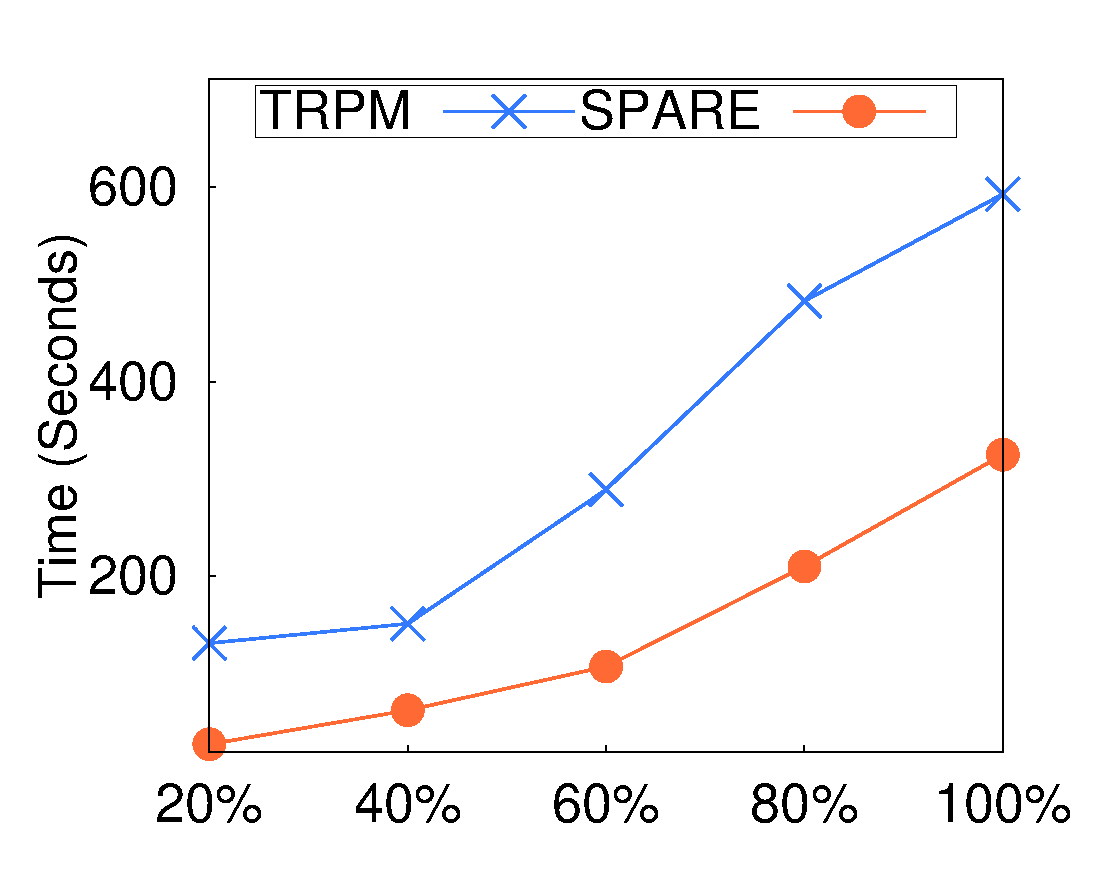
\includegraphics[width=\textwidth]{/exp/performance/shopping_vary_o.eps}
        \caption{Shopping vary $O_r$}
    \end{subfigure}
        \begin{subfigure}[b]{0.16\textwidth}
	 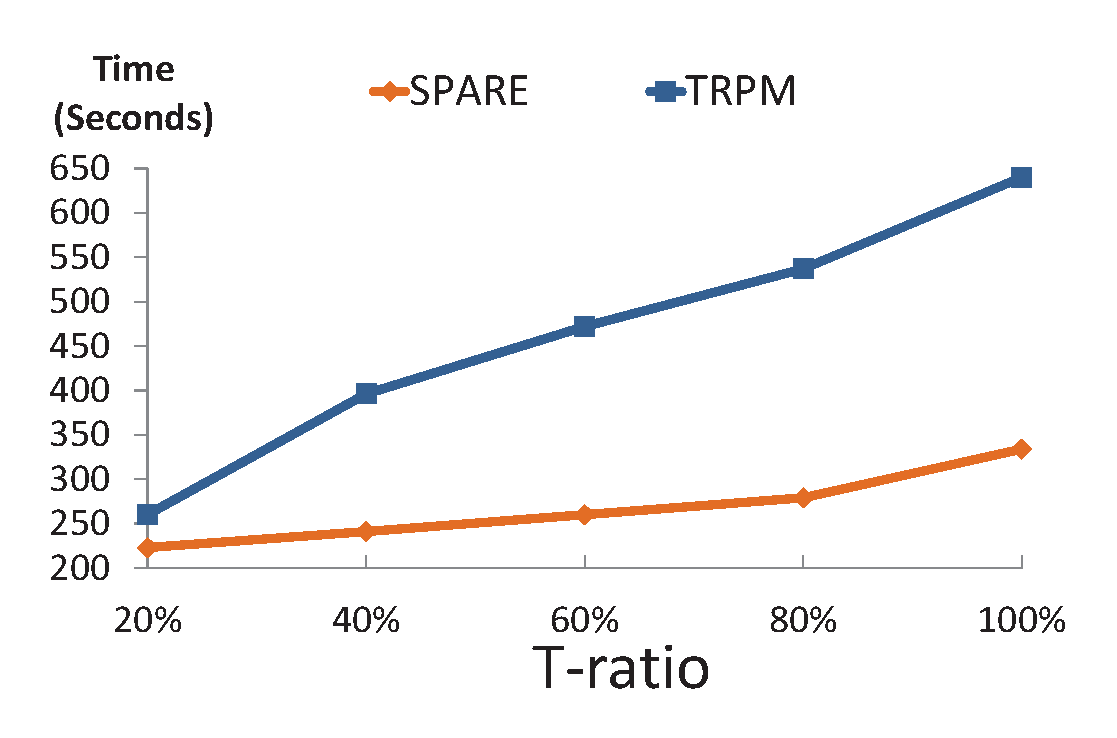
\includegraphics[width=\textwidth]{/exp/performance/shopping_vary_t.eps}
        \caption{Shopping vary $T_r$}
    \end{subfigure}
        
	\begin{subfigure}[b]{0.16\textwidth}
        \includegraphics[width=\textwidth]{/exp/performance/geolife_vary_M.eps}
        \caption{GeoLife vary $M$}
    \end{subfigure}
    \begin{subfigure}[b]{0.16\textwidth}
        \includegraphics[width=\textwidth]{/exp/performance/geolife_vary_K.eps}
        \caption{GeoLife vary $K$}
    \end{subfigure}
    \begin{subfigure}[b]{0.16\textwidth}
        \includegraphics[width=\textwidth]{/exp/performance/geolife_vary_L.eps}
        \caption{GeoLife vary $L$}
    \end{subfigure}
       \begin{subfigure}[b]{0.16\textwidth}
        \includegraphics[width=\textwidth]{/exp/performance/geolife_vary_G.eps}
        \caption{GeoLife vary $G$}
    \end{subfigure}       
 	 \begin{subfigure}[b]{0.16\textwidth}
        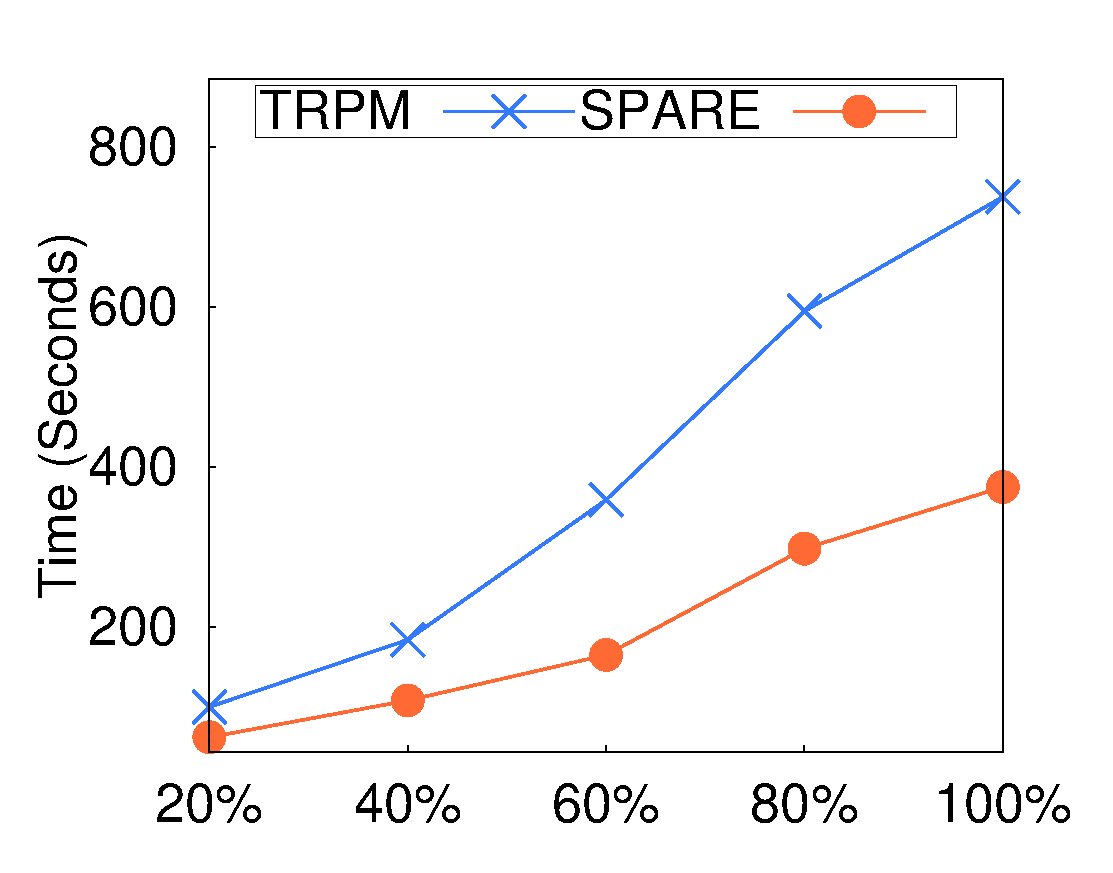
\includegraphics[width=\textwidth]{/exp/performance/geolife_vary_o.eps}
        \caption{GeoLife vary $O_r$}
    \end{subfigure}
 	\begin{subfigure}[b]{0.16\textwidth}
        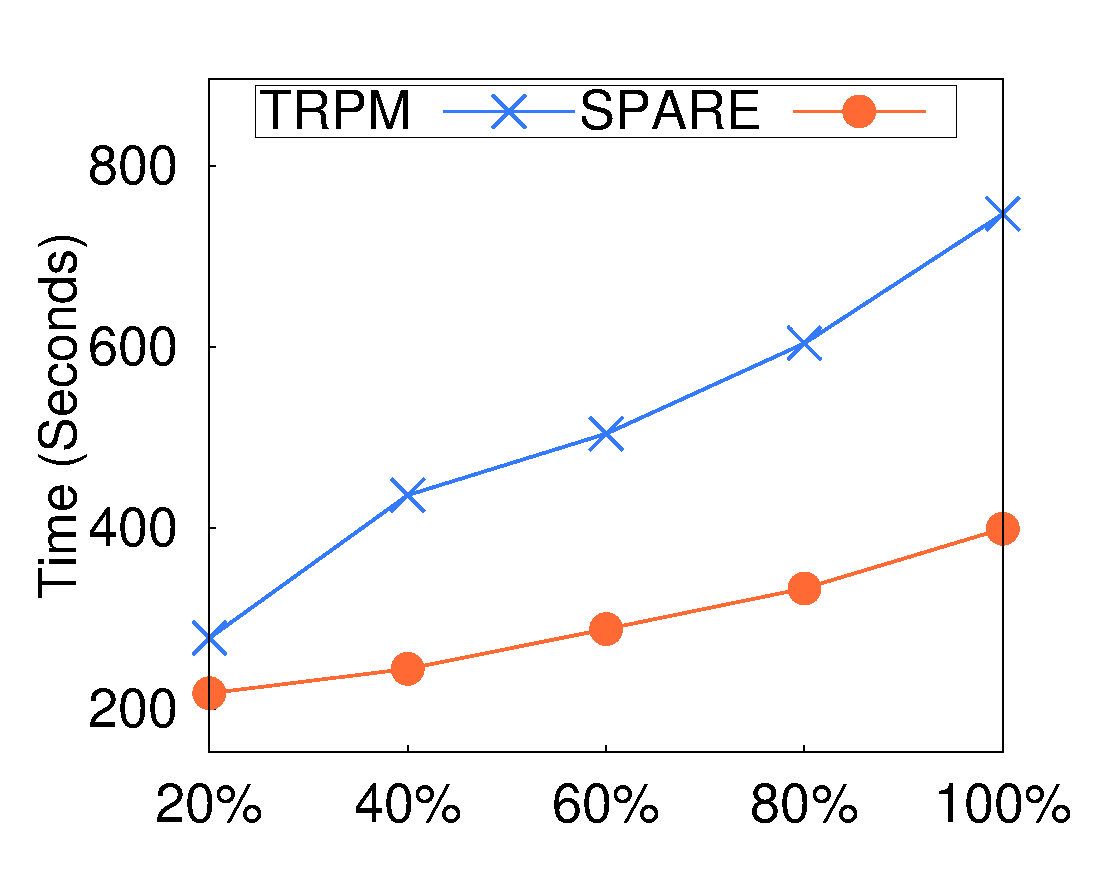
\includegraphics[width=\textwidth]{/exp/performance/geolife_vary_t.eps}
        \caption{GeoLife vary $T_r$}
    \end{subfigure}    
    
    \begin{subfigure}[b]{0.16\textwidth}
        \includegraphics[width=\textwidth]{/exp/performance/taxi_vary_M.eps}
        \caption{Taxi vary $M$}
    \end{subfigure}
    \begin{subfigure}[b]{0.16\textwidth}
        \includegraphics[width=\textwidth]{/exp/performance/taxi_vary_K.eps}
        \caption{Taxi vary $K$}
    \end{subfigure}
    \begin{subfigure}[b]{0.16\textwidth}
        \includegraphics[width=\textwidth]{/exp/performance/taxi_vary_L.eps}
        \caption{Taxi vary $L$}
    \end{subfigure}
       \begin{subfigure}[b]{0.16\textwidth}
        \includegraphics[width=\textwidth]{/exp/performance/taxi_vary_G.eps}
        \caption{Taxi vary $G$}
    \end{subfigure}   
	 \begin{subfigure}[b]{0.16\textwidth}
        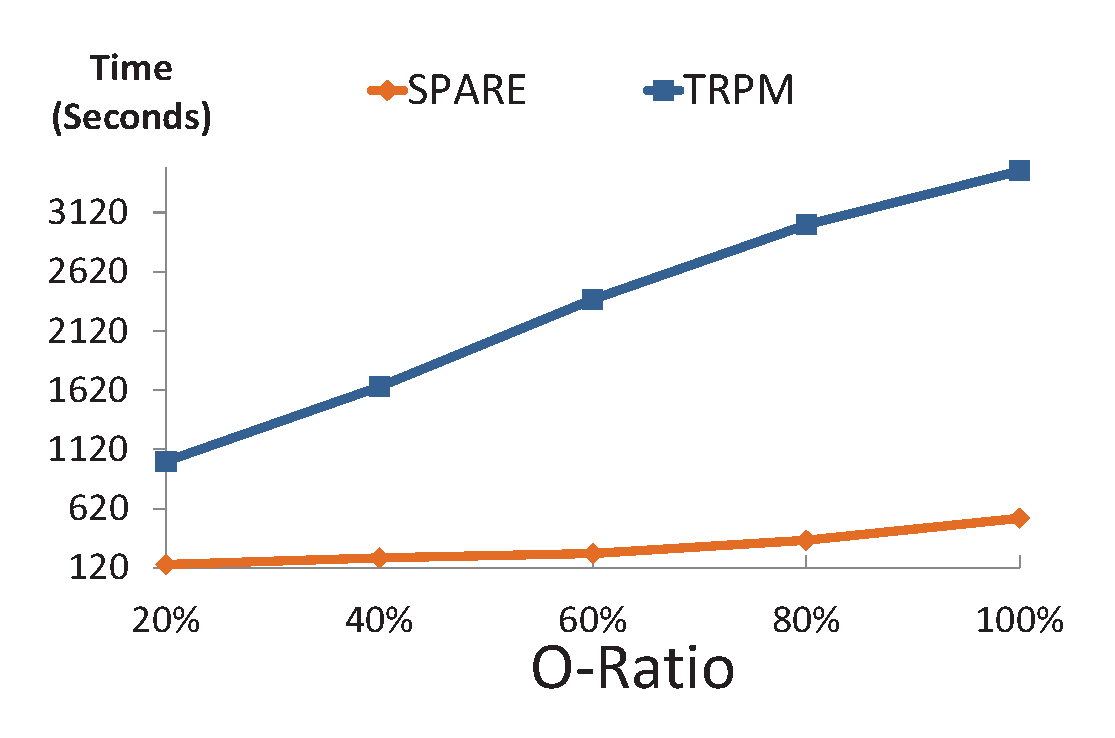
\includegraphics[width=\textwidth]{/exp/performance/taxi_vary_o.eps}
        \caption{Taxi vary $O_r$}
    \end{subfigure}
    	 \begin{subfigure}[b]{0.16\textwidth}
        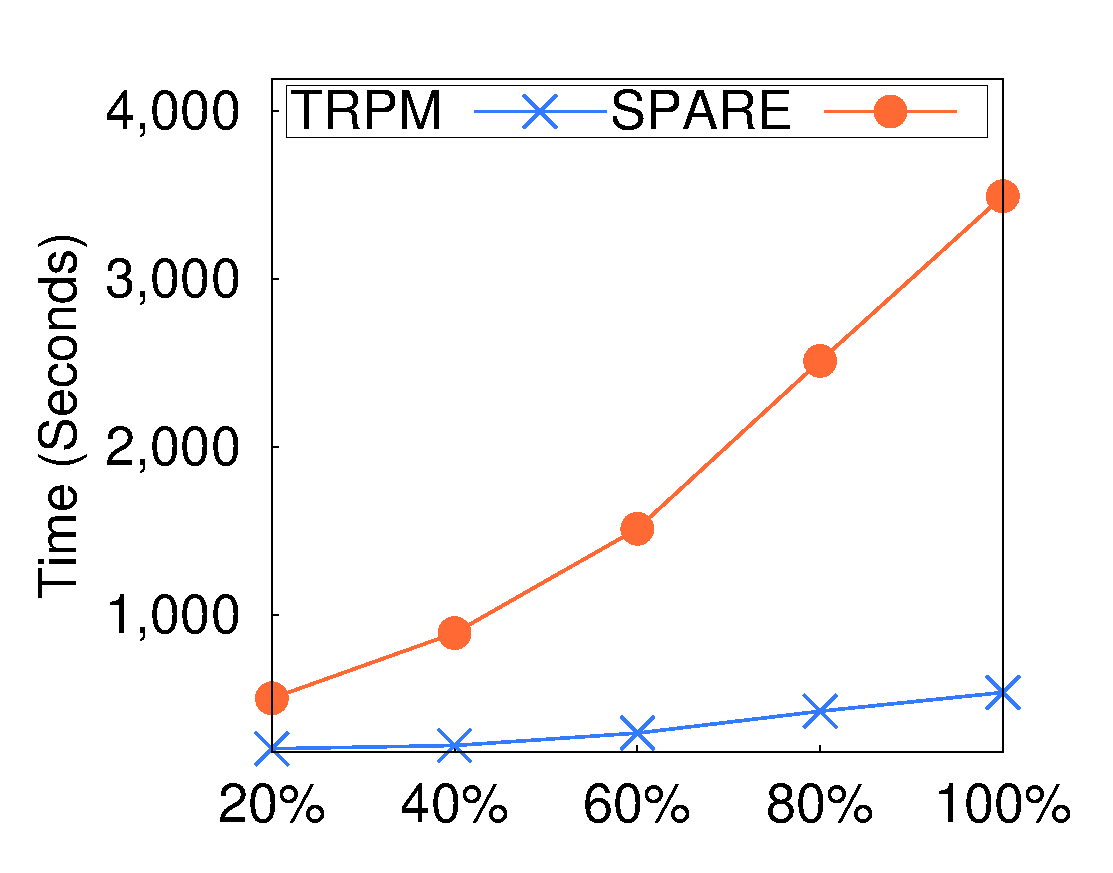
\includegraphics[width=\textwidth]{/exp/performance/taxi_vary_t.eps}
        \caption{Taxi vary $T_r$}
    \end{subfigure}      
        
\caption{Performance of SPARE and TRPM on real datasets under different pattern parameters.}
\label{exp:performance_vary}
\end{figure*}
\textbf{Varying $M$}: Figures~\ref{exp:performance_vary} (a),(g),(m)
present the performance with increasing $M$. The SPARE framework demonstrates a clear superiority over the TRPM framework, with 
a performance gain by a factor of  $2.7$ times in Shopping, $3.1$ times in GeoLife and
$7$ times in Taxi. As $M$ increases, the running time of both frameworks slightly improve because the number of clusters in each snapshot drops, generating fewer valid candidates.

\textbf{Varying $K$}: The performance with increasing $K$ is shown in Figure~\ref{exp:performance_vary} (b),(h),(n).  SPARE tends to run faster, whereas the performance of TRPM degrades dramatically. This is caused by the \emph{sequence simplification} procedure in SPARE, which can prune many candidates with large $K$. However, the line sweep algorithm in TRPM does not utilize such property for pruning. It takes longer time because more replicated data has to be handled in each partition.

\textbf{Varying $L$}: Figures~\ref{exp:performance_vary} (c),(i),(o) present the performances with increasing $L$. When $L=10$, SPARE can outperform TRPM by around $10$ times. We also observe that there is a significant performance improvement for TPRM when $L$ increases from $10$ to $20$ and later the running time drops smoothly. 
This is because $\eta$ is proportional to $O(K*G/L+L)$. When $L$ is small (i.e., from $10$ to $20$),
$\eta$ decreases drastically. As $L$ increases, $\eta$ varies less significantly.

\textbf{Varying $G$}: Figures~\ref{exp:performance_vary} (d),(j),(p) present the performances with increasing $G$.  TRPM is rather sensitive to $G$. When $G$ is relaxed to larger values, more valid patterns would be generated. TPRM has to set a higher replication factor and its running time degrades drastically when $G$ increases from $20$ to $30$. In contrast, with much more effective pruning strategy, our SPARE scales well with $G$. Particularly, SPARE is 14 times faster than TRPM when $G=20$ in GeoLife dataset.

\textbf{Varying $O_r$}: Figures~\ref{exp:performance_vary} (e),(k),(q) present the performances with increasing number of moving objects. Both TRPM and SPARE take longer time to find patterns in a larger database. We can see that the performance gap between SPARE and TRPM is widened as more objects are involved, which shows SPARE is more scalable.

\textbf{Varying $T_r$}: Figures~\ref{exp:performance_vary} (f),(l),(r) present 
the performances with increasing number of snapshots. As $T_r$ increases, SPARE scales much better than TRPM due to its effective pruning in the temporal dimension. 

\revised{
\textbf{Resources}: Table~\ref{tbl:resource} lists the system resources taken by TRPM and SPARE under the default setting. Both TRPM and SPARE are resource efficient as they only occupy less than 20\% 
of the available memory which reveals their potential to handle larger trajectories. Again, SPARE outperforms TRPM in both execution time and memory usage which dues
to the set of effective pruning procedures.

\begin{table}[h]
\small
\begin{tabular}{|l|c|c|c|c|}
\hline
\multicolumn{1}{|c|}{\textbf{Dataset}} & \textbf{Method} & \textbf{Time} & \textbf{Vcore-seconds} & \textbf{Memory} \\ \hline
\multirow{2}{*}{Shopping}              & TRPM            & 597                               & 90,859                 & 10,019               \\ \cline{2-5} 
                                       & SPARE           & 334                               & 47,430                 & 8,613                \\ \hline
\multirow{2}{*}{Geolife}               & TRPM            & 747                               & 106,428                & 18,454               \\ \cline{2-5} 
                                       & SPARE           & 480                               & 49,835                 & 14,369               \\ \hline
\multirow{2}{*}{Taxi}                  & TRPM            & 3,648                             & 503,460                & 51,691               \\ \cline{2-5} 
                                       & SPARE           & 812                               & 89,390                 & 35,912               \\ \hline
\end{tabular}
\caption{Resources taken for TRPM and SPARE. Time is in seconds representing observed performance. Vcore-seconds is the aggregate of time spent in each core. Memory is in MB representing the actual size of RDDs.}
\label{tbl:resource}
\end{table}
}
%\begin{figure}[h]
%\centering
%	\begin{subfigure}[b]{0.22\textwidth}
%	 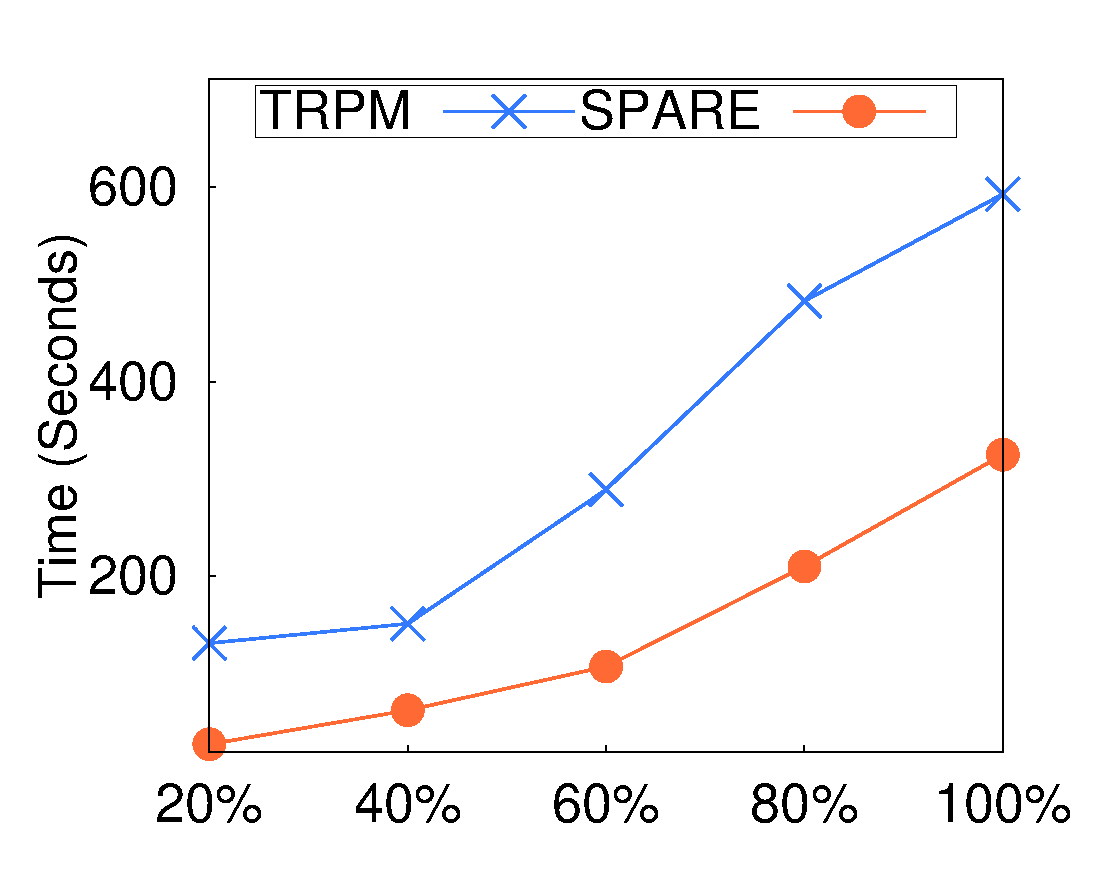
\includegraphics[width=\textwidth]{/exp/performance/shopping_vary_o.eps}
%        \caption{Shopping vary $O_r$}
%    \end{subfigure}
% 	 \begin{subfigure}[b]{0.22\textwidth}
%        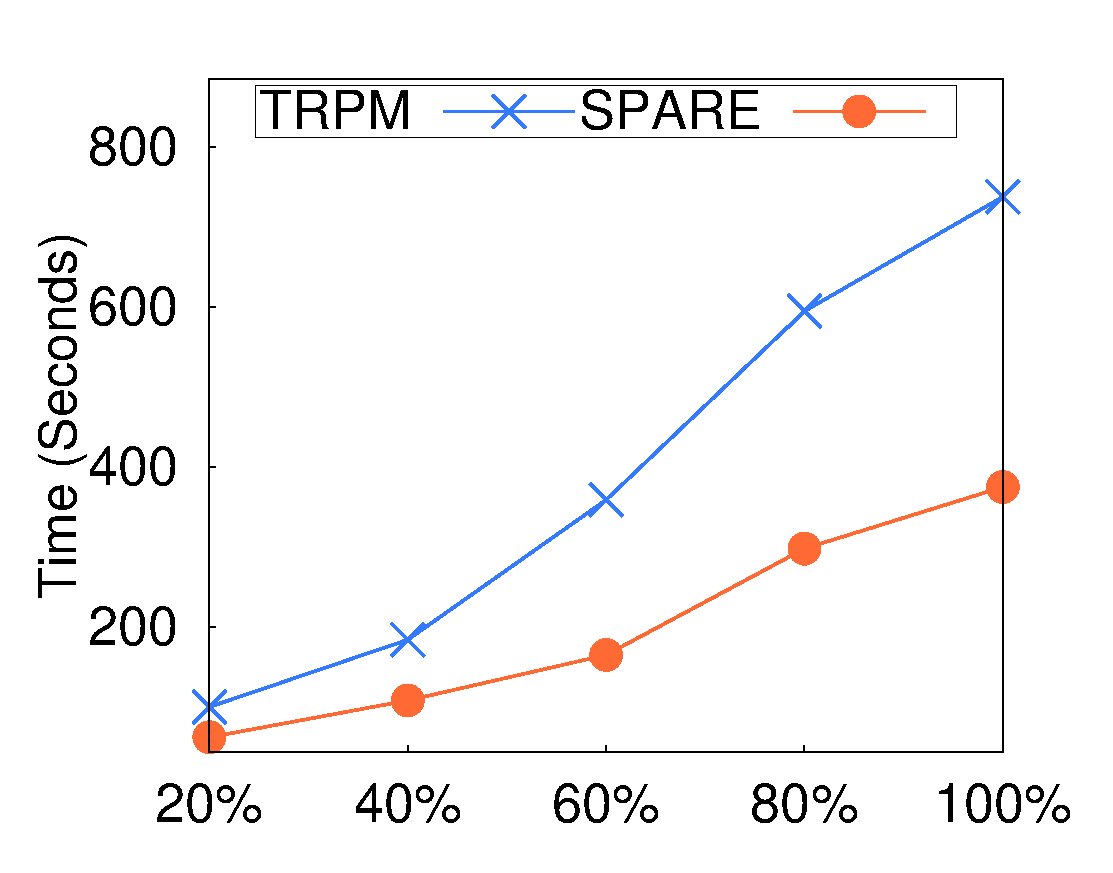
\includegraphics[width=\textwidth]{/exp/performance/geolife_vary_o.eps}
%        \caption{Geolife vary $O_r$}
%    \end{subfigure}
%    	 \begin{subfigure}[b]{0.22\textwidth}
%        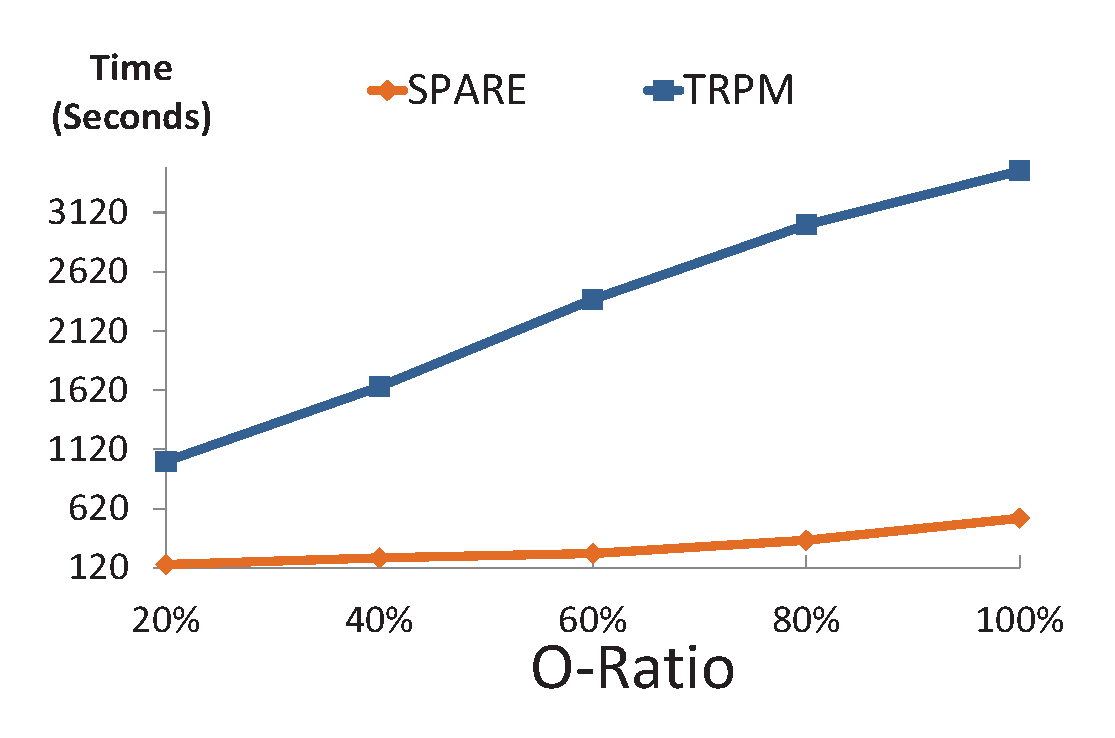
\includegraphics[width=\textwidth]{/exp/performance/taxi_vary_o.eps}
%        \caption{Taxi vary $O_r$}
%    \end{subfigure}
%    \begin{subfigure}[b]{0.22\textwidth}
%	 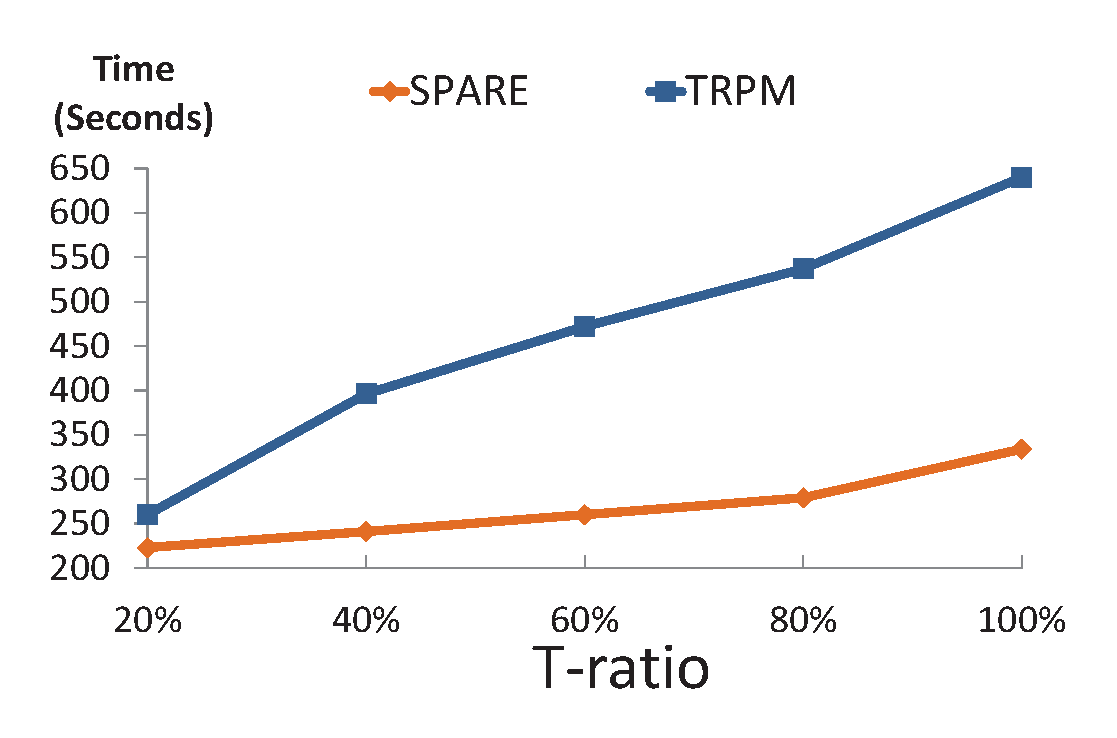
\includegraphics[width=\textwidth]{/exp/performance/shopping_vary_t.eps}
%        \caption{Shopping vary $T_r$}
%    \end{subfigure}
% 	 \begin{subfigure}[b]{0.22\textwidth}
%        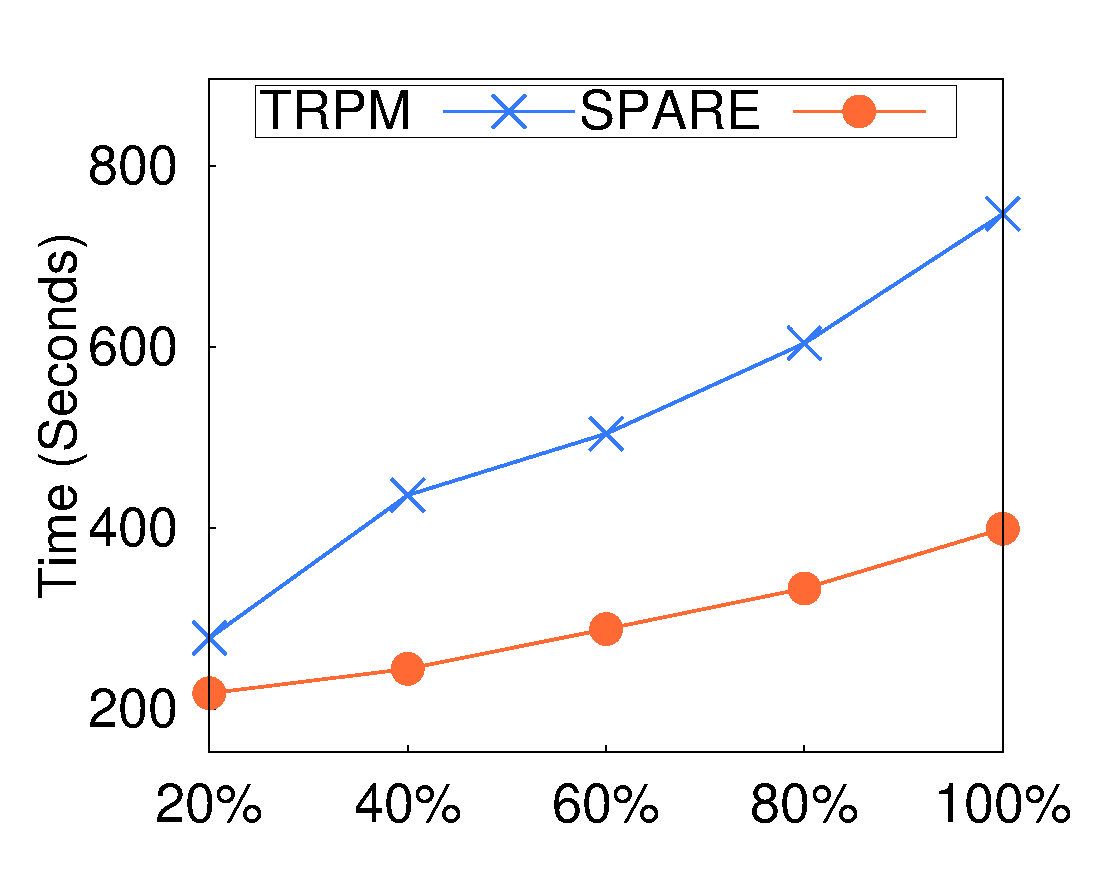
\includegraphics[width=\textwidth]{/exp/performance/geolife_vary_t.eps}
%        \caption{Geolife vary $T_r$}
%    \end{subfigure}
%    	 \begin{subfigure}[b]{0.22\textwidth}
%        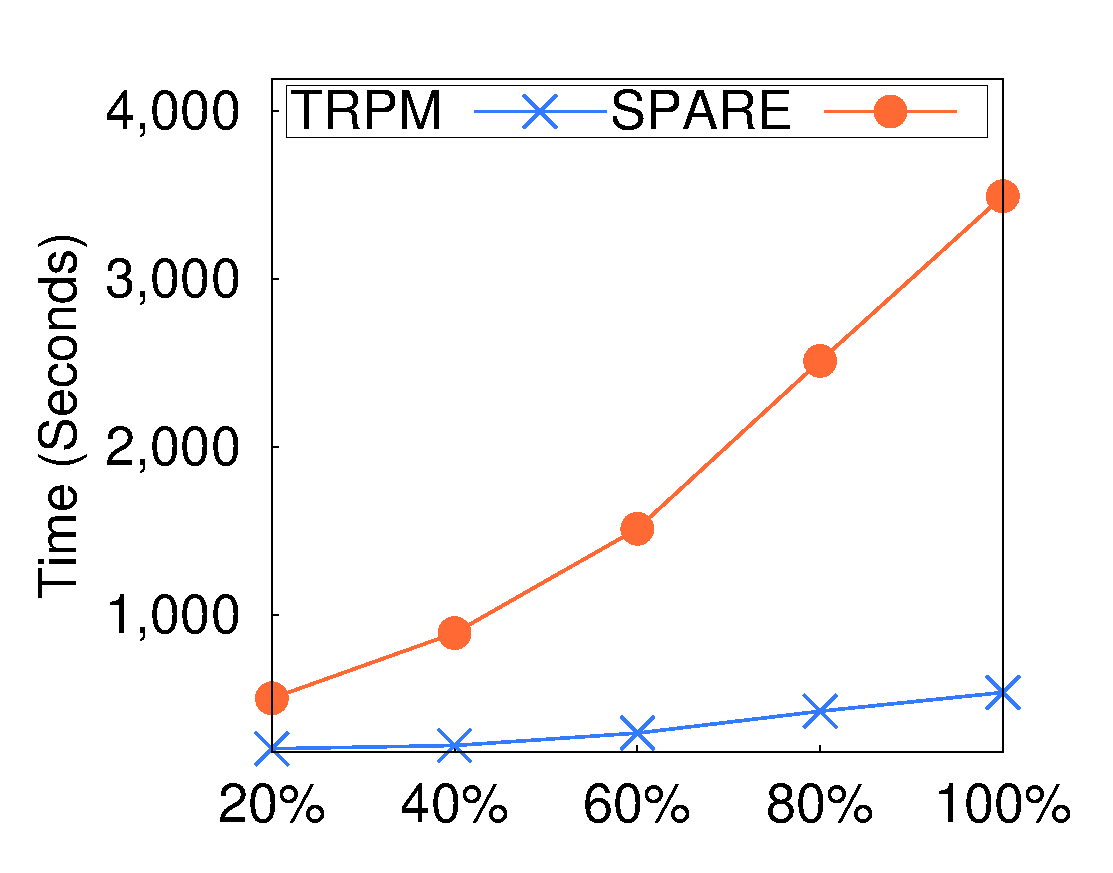
\includegraphics[width=\textwidth]{/exp/performance/taxi_vary_t.eps}
%        \caption{Taxi vary $T_r$}
%    \end{subfigure}
% \caption{Scalability of SPARE and TRPM wrt. $O_r$ and $T_r$}
% \label{exp:performance_vary_OT}
%\end{figure}



\subsection{Analysis of SPARE framework}
In this part, we extensively evaluate SPARE from three aspects:
(1) the advantages brought by the sequence simplification, (2) the effectiveness of load balance, and (3) the scalability with increasing computing resources.
%Then, we study the scalability of SPARE with increasing computing resources.


\subsubsection{Power of sequence simplification}
To study the power of sequence simplification,
we collect two types of statistics: (1) the number of pairs that
are shuffled to the reducers and (2) the number of pairs that
are fed to the Apirori Enumerator. The difference between these two values is the number of size-$2$ candidates pruned by the sequence simplification.
The results in Table~\ref{tbl:pruning} show that the \emph{sequence simplification} is very powerful and eliminates nearly 90 percent of the object pairs, which significantly reduces the overhead of subsequent Apriori enumerator.

\begin{table}[h]
\centering
\begin{tabular}{|l|c|c|c|}
\hline 
\textbf{Dataset} & \textbf{Shopping} & \textbf{GeoLife} & \textbf{Taxi} \\ 
\hline 
Before pruning & 878,309 &  1,134,228 & 2,210,101 \\ 
\hline 
After pruning & 76,672 & 123,410 & 270,921 \\ 
\hline 
Prune ratio & 91.2\% & 89.1\% & 87.7\% \\ 
\hline 
\end{tabular} 

\caption{Pruning power of SPARE.}
\label{tbl:pruning}
\end{table}

\begin{figure}[h]
\centering
	  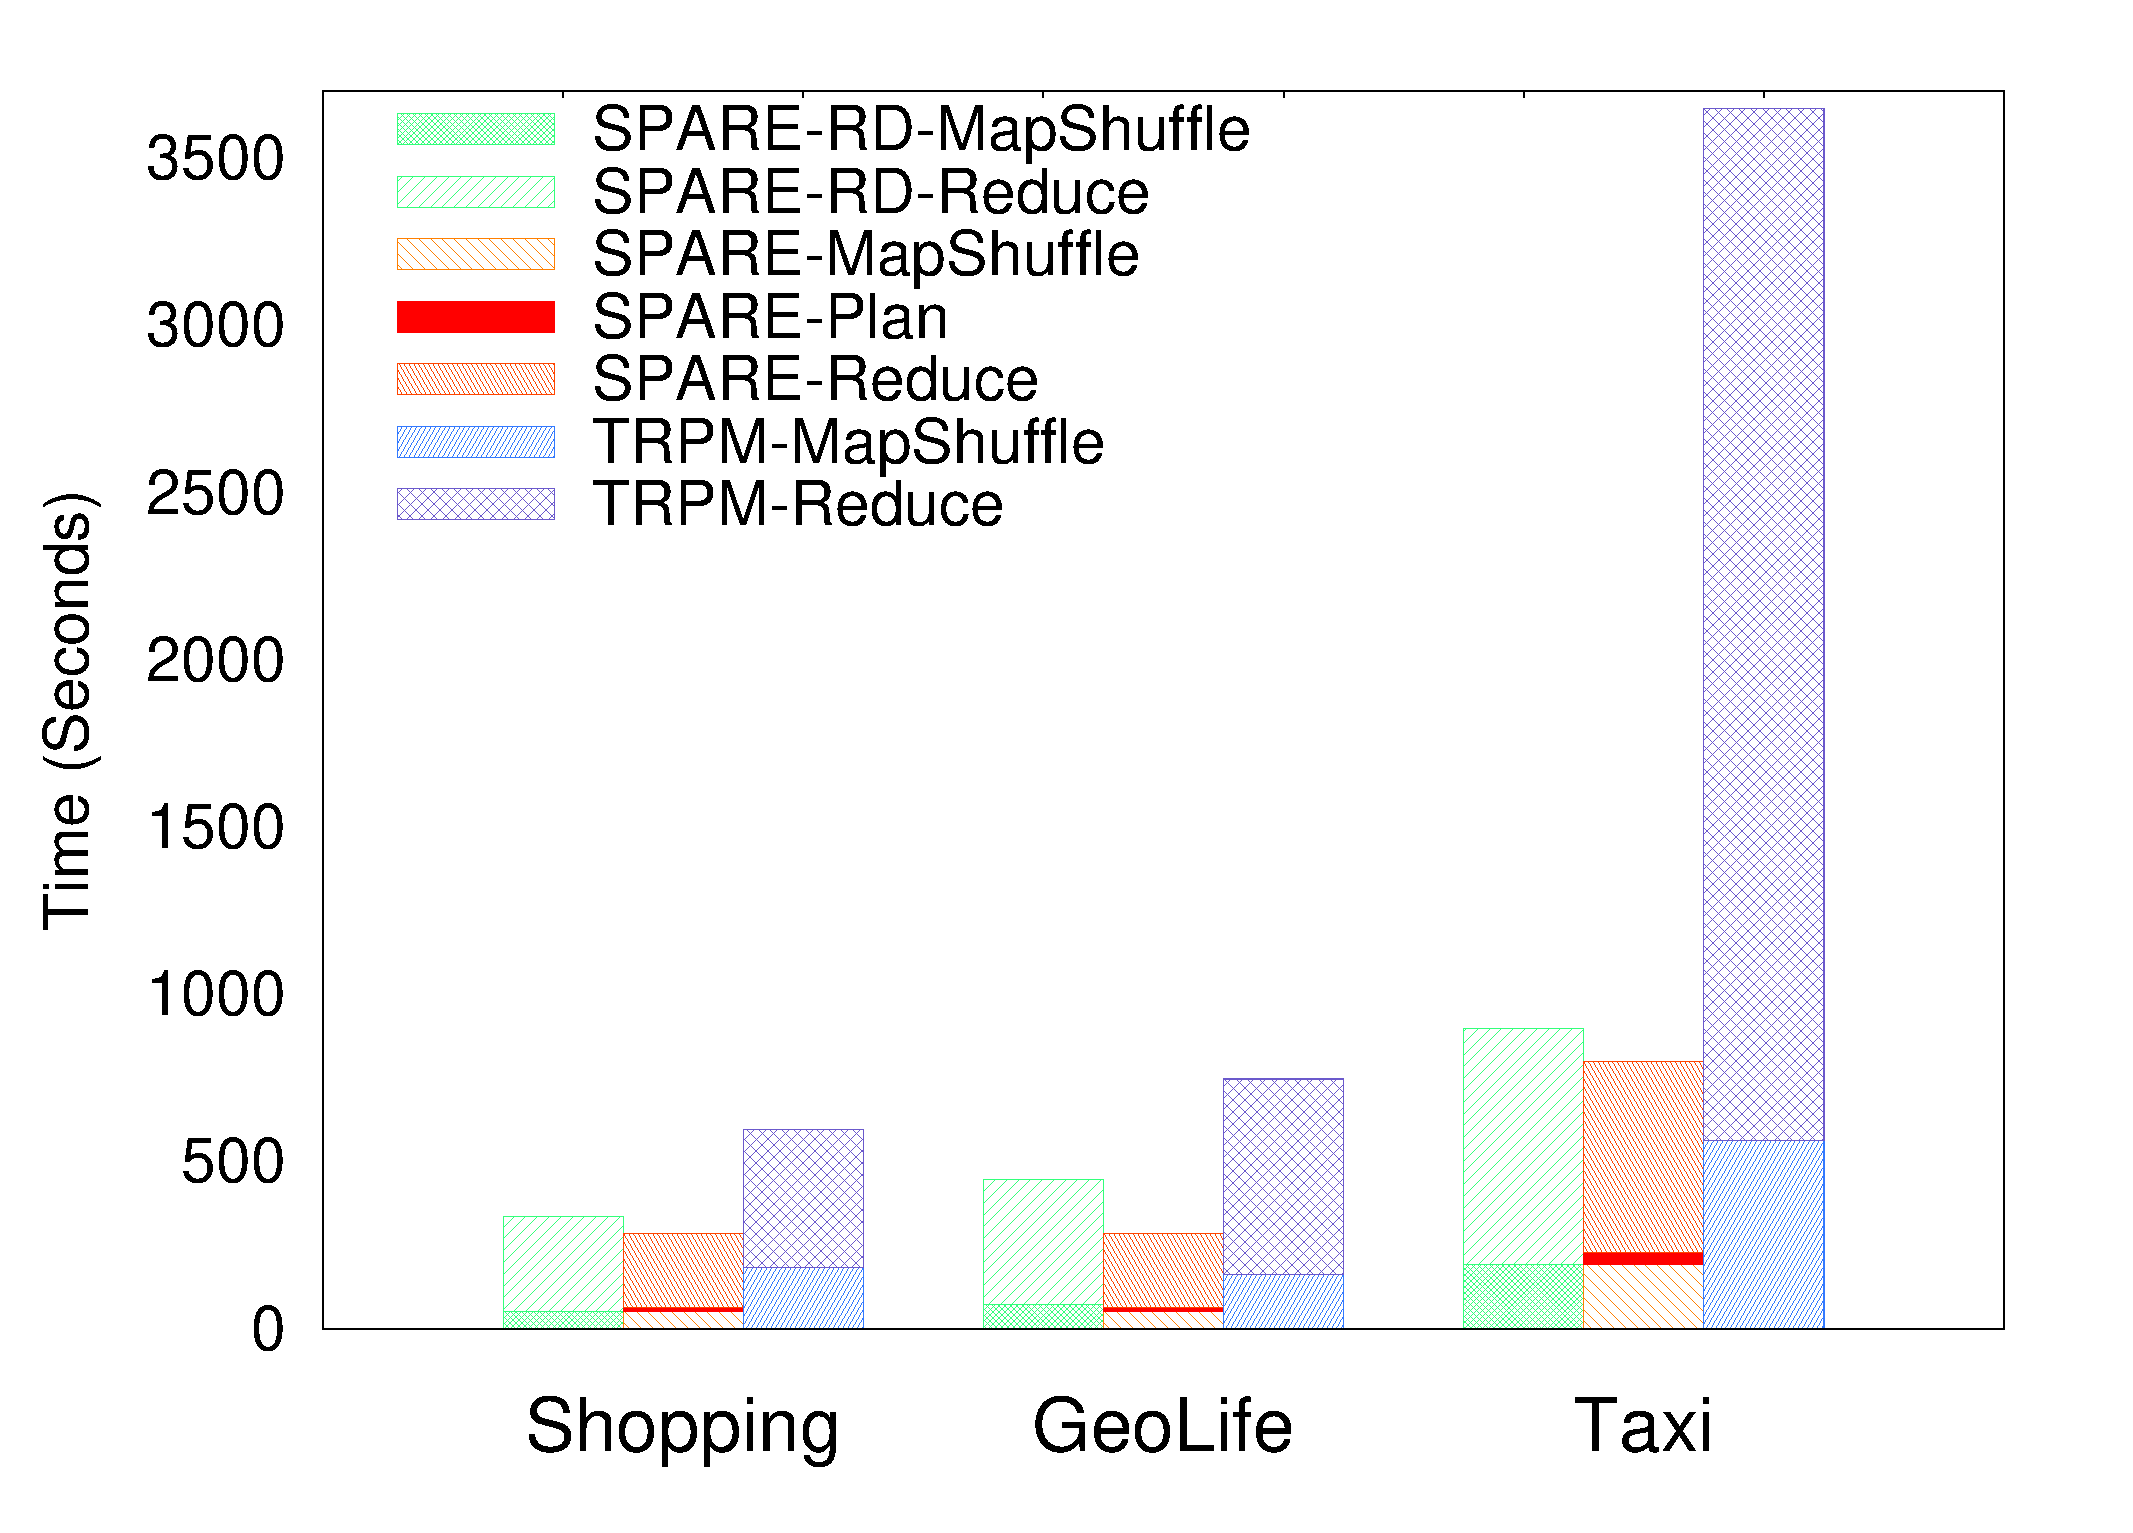
\includegraphics[width=0.35\textwidth]{/exp/spare/detail1.eps}
    \caption{Breakdown of cost of TRPM, SPARE and SPARE-RD.}
    \label{exp:wl}
\end{figure}

\begin{table}[h]
\centering \small
\begin{tabular}{|c|c|c|c|c|}
\hline
\multirow{2}{*}{\textbf{Dataset}} & \multicolumn{2}{c|}{\textbf{SPARE-RD}} & \multicolumn{2}{c|}{\textbf{SPARE}} \\ \cline{2-5} 
                         & Straggler        & Std. Dev.     & Straggler       & Std. Dev.      \\ \hline
Shopping                 & 295              & 41         & 237             & 21       \\ \hline
GeoLife                  & 484              & 108        & 341             & 56       \\ \hline
Taxi                     & 681              & 147        & 580             & 96       \\ \hline
\end{tabular}
  \caption{Statistics of execution time (in seconds) among executors.}
  \label{tbl:strags}
\end{table}

\subsubsection{Load balance}
To study the effect of load balance in the SPARE framework, we use random task allocation (the default setting of Spark) as a baseline, denoted by SPARE-RD, and compare it with our best-fit method. In best-fit, the largest unassigned star is allocated to the currently most lightly loaded reducer.
Figure~\ref{exp:wl} shows the breakdown of the costs in the map-reduce stages for SPARE and SPARE-RD \revised{with TRPM as comparison}. We observe that the map and shuffle time of SPARE and SPARE-RD are identical . The difference is that SPARE incurs an additional overhead to generate an allocation plan for load balance (around $4\%$ of the total cost), resulting in significant savings in the reduce stage (around $20\%$ of the total cost). \revised{We further observe that TRPM takes more time in each phase, which confirms the efficiency of Star Partition and Apriori Enumeration.} We also report the cost of \emph{straggler}, i.e., the longest job, and the standard deviation (Std. Dev.) for all jobs in Table~\ref{tbl:strags}, whose results clearly verify the effectiveness of our allocation strategy for load balance.

\subsubsection{Scalability}
When examining SPARE with increasing computing resources (number of machines), we also compare SPARE with the state-of-the-art solutions for \emph{swarm} and \emph{platoon} in the single-node setting. Since the original \emph{swarm} and \emph{platoon} detectors cannot handle very large-scale datasets, we only use 60\% of each dataset for evaluation. To make fair comparisons, we customize two variants of SPARE to mine \emph{swarm}s and \emph{platoon}s, which are denoted as SPARE-S and SPARE-P respectively. The customization is according to the settings in Table~\ref{tbl:patterns} and the results are reported in Figure~\ref{exp:scalability}. 
First, the centralized schemes are not suitable to discover patterns in 
large-scale trajectory databases. It takes nearly $30$ hours to 
detect \emph{swarm}s and $11$ hours to detect \emph{platoon}s in the Taxi dataset in a single machine. 
In contrast, when utilizing the multi-core \revised{(i.e., single node with 3 executors)} environment, 
SPARE-P achieves $7$ times speedup and SPARE-S achieves $10$ times speedup. 
%our TRPM and SPARE achieves 2.4 times and 7.1 times speedup respectively. 
Second, we see that SPARE schemes demonstrate promising scalability in terms of the number of machines available. The running times decrease almost inversely as more machines are used. 
When all the $11$ nodes ($162$ cores) are available, 
SPARE-P is upto $65$ times and SPARE-S is upto $112$ times better than the state-of-the-art centralized schemes.
%than \emph{platoon} and SPARE-S is upto $112$ times better than \emph{swarm}.
%state-of-the-art \emph{platoon} detector in a centralized server.

\begin{figure*}[t]
\centering
\begin{subfigure}[b]{0.31\textwidth}
    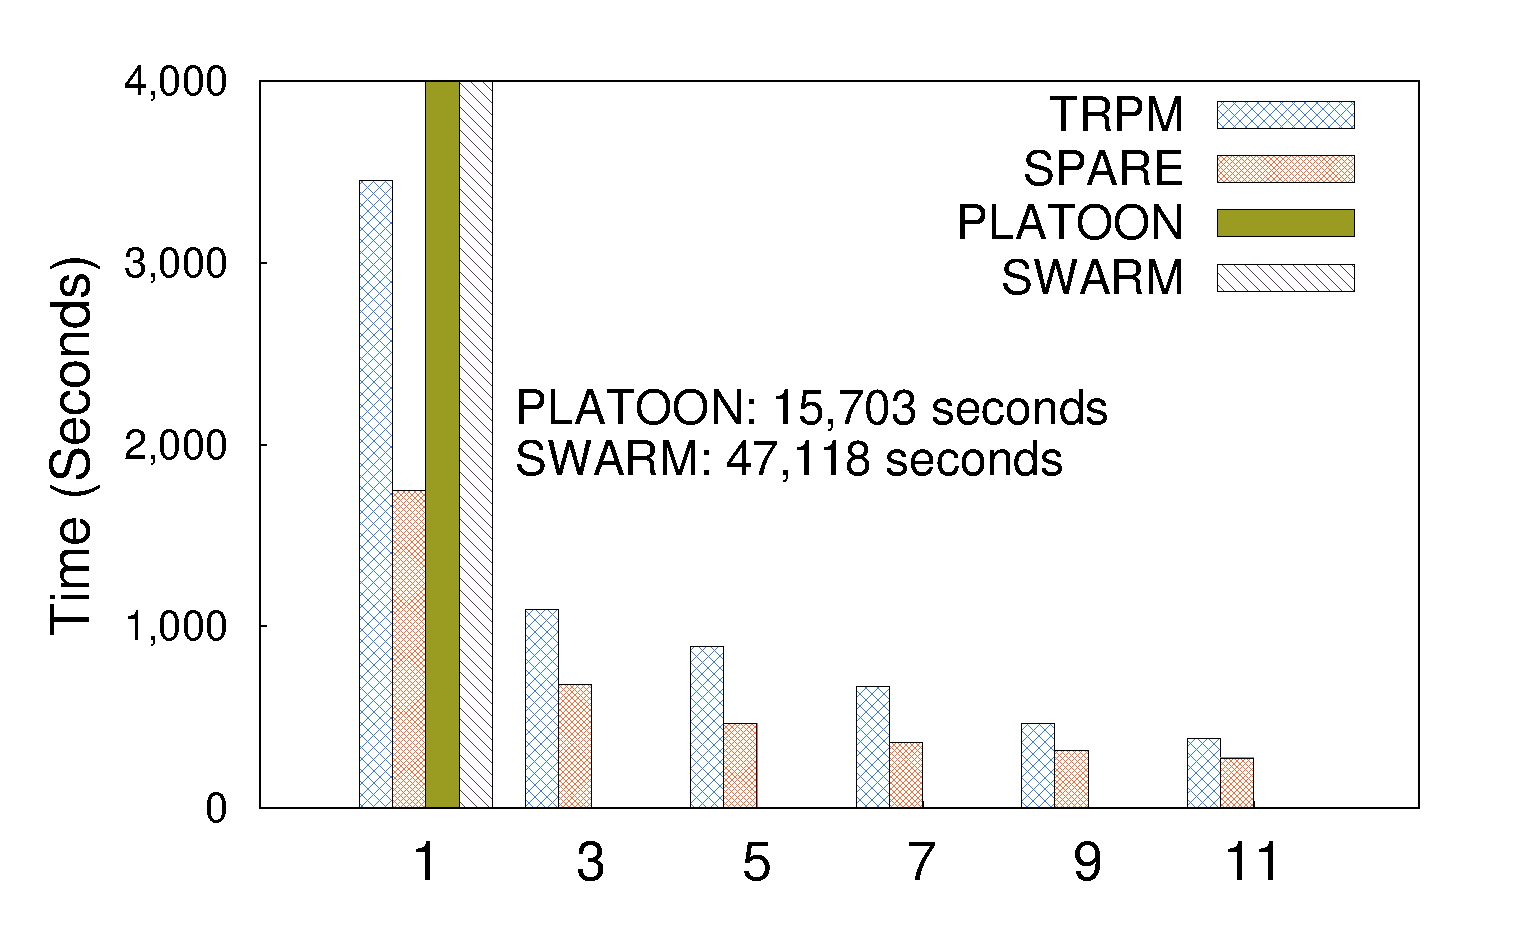
\includegraphics[width=\textwidth]{/exp/spare/scalability-shopping.eps}
        \caption{Shopping vary $N$}
    \end{subfigure}
 	 \begin{subfigure}[b]{0.31\textwidth}
        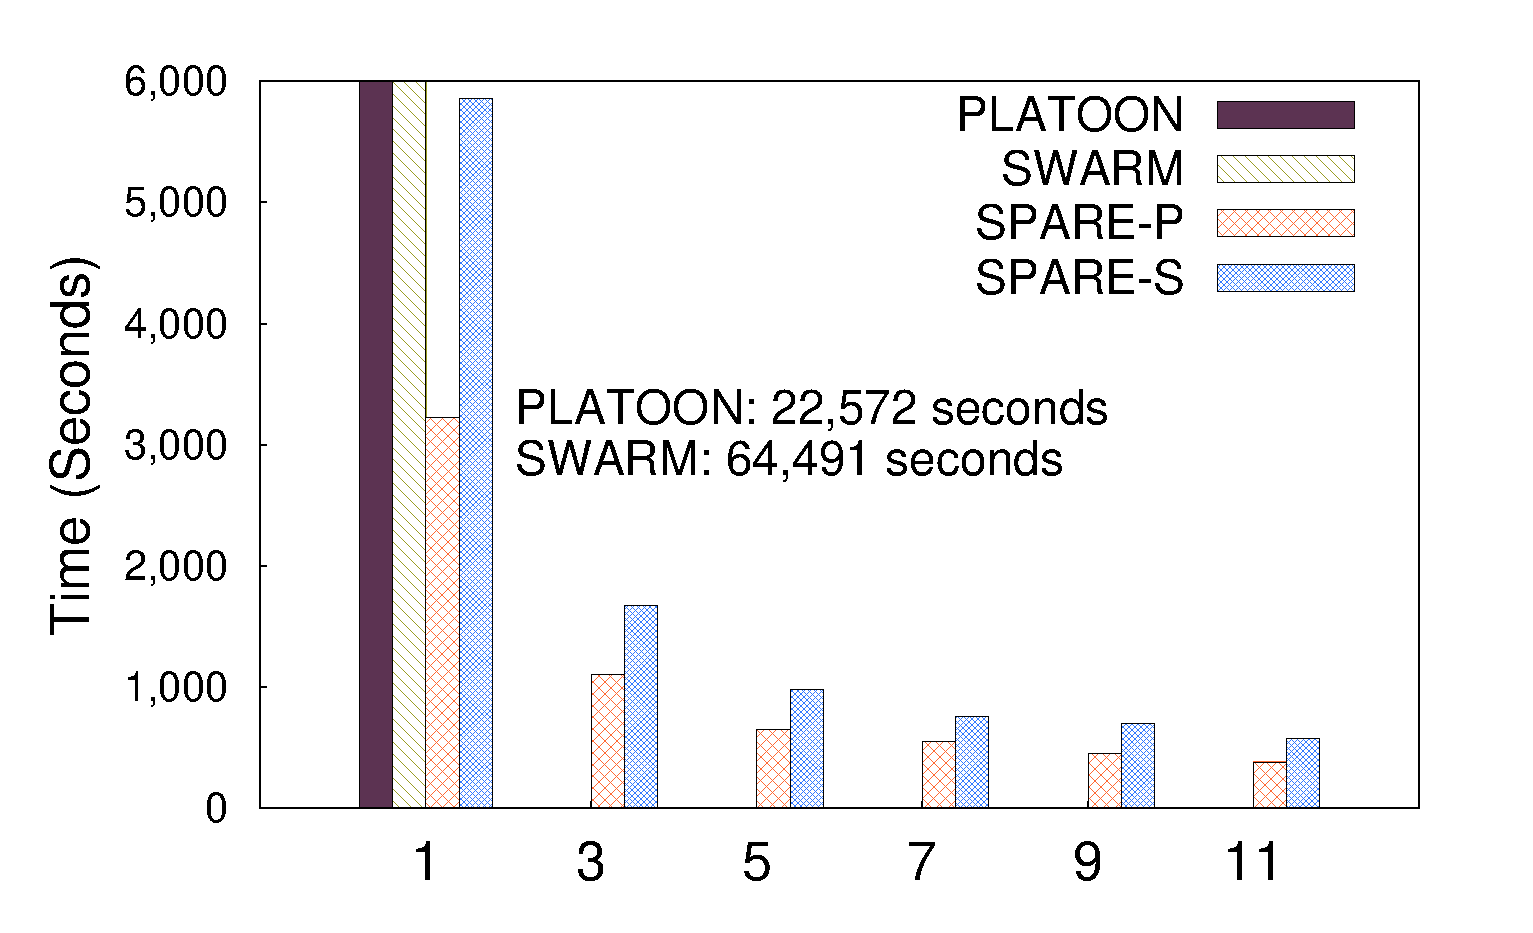
\includegraphics[width=\textwidth]{/exp/spare/scalability-geolife.eps}
        \caption{GeoLife vary $N$}
    \end{subfigure}
    	 \begin{subfigure}[b]{0.31\textwidth}
        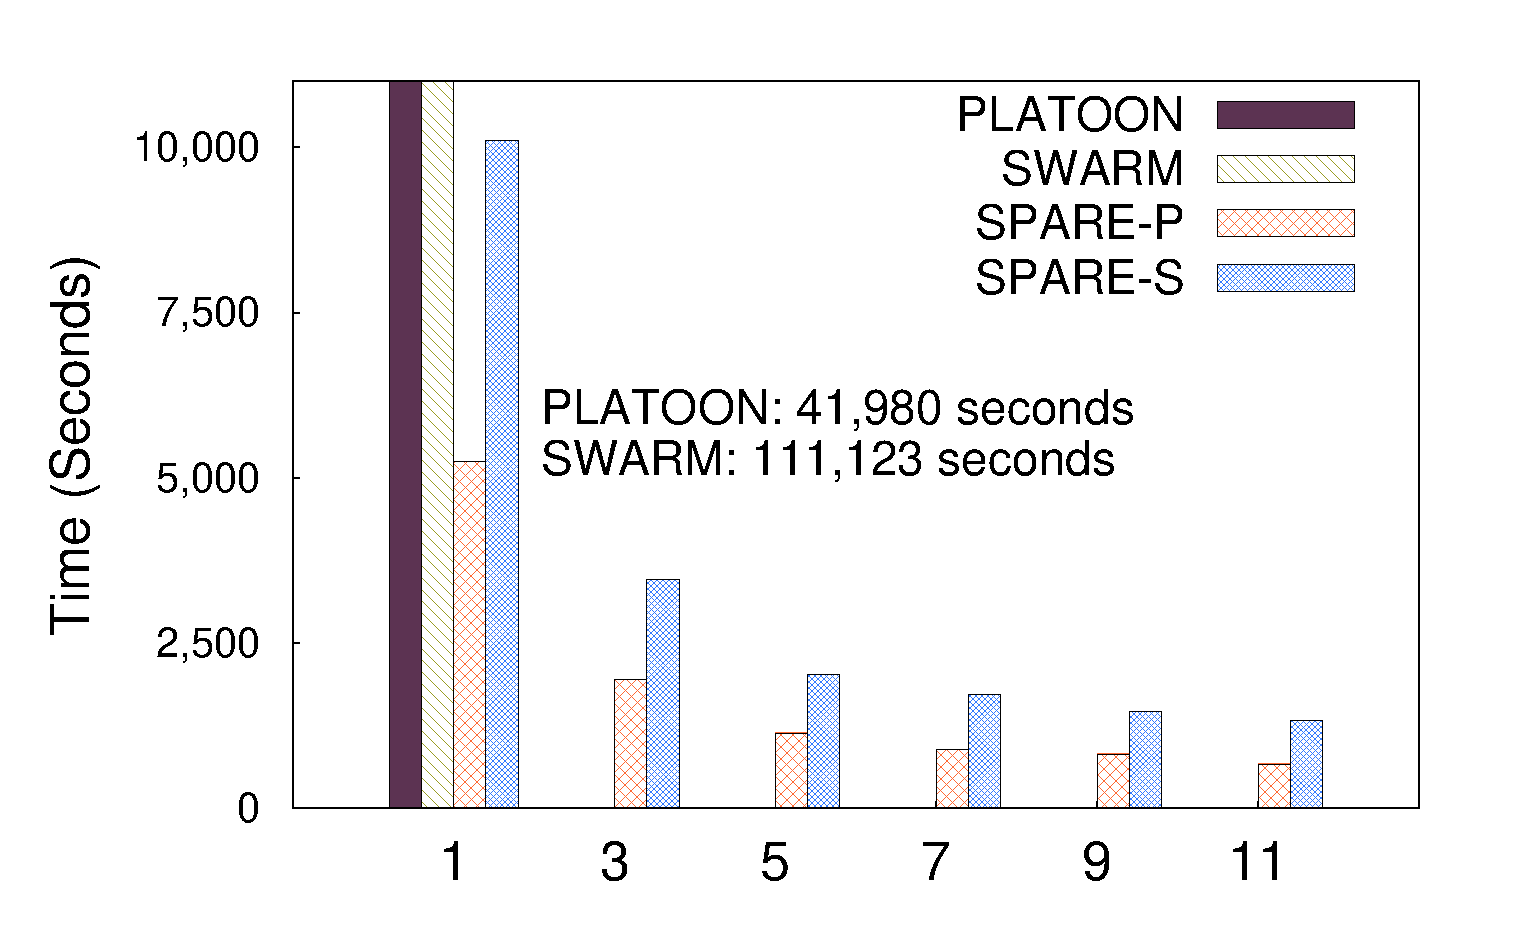
\includegraphics[width=\textwidth]{/exp/spare/scalability-taxi.eps}
        \caption{Taxi vary $N$}
    \end{subfigure}
 \caption{Comparisons among TRMP, SPARE, PLATOON and SWARM.}
 \label{exp:scalability}
\end{figure*}

\section{Conclusions and Future Work}
\label{sec:concl}
In this paper, we proposed a generalized co-movement pattern to unify those proposed in the past literature. We also devised two types of parallel frameworks in Spark that can scale to support pattern detection in a trajectory database with hundreds of millions of points. The efficiency and scalability were verified by extensive experiments on three real datasets. In the future work, we are interested to examine co-movement pattern detection in streaming data for real-time monitoring. How to extend the current parallel framework to support other types of advanced patterns is also of interest.

% The following two commands are all you need in the
% initial runs of your .tex file to
% produce the bibliography for the citations in your paper.
\bibliographystyle{IEEEtr}
\small
\bibliography{citations}
\appendix
\section{Proofs of Theorems}
%\subsection{Proof of Theorem~\ref{THM:RP_ETA}} 
%\label{appx:proof-rp-eta}
%\begin{proof}
%We compute $\eta$ by analyzing $\range(\rho_{G,L,K}(\cdot))$.
%In the following, when no ambiguity, we use $\rho(T)$ to represent
%$\rho_{G,L,K}(T)$. For any sequence $T$, its $\rho(T)$ can
%be viewed as interleaving segments and gaps. 
%We may view $\rho(T)$ as $l_1,g_1,\ldots, l_{n-1}, g_{n-1}, l_n$, where $l_i$ is a
%segment and $g_i$ is a gap. For simplicity, we use $l_i$ and $g_i$ directly as their sizes.
%Then the
%range of $\rho(T)$ is $\Sigma_{i=1}^{i=n} l_i + \Sigma_{i=1}^{i=n-1} g_i$. 
%Since $\rho(T)$ is valid, the following constraints holds: 
%(1) $\Sigma_{i=1}^{i=n} l_i \geq K$; (2) $\forall l_i$, $l_i \geq L$;
%(3) $\forall g_i$, $g_i \leq G-1$. Based on constraint (1) and (2), 
%$n \leq \lceil \frac{K}{L}\rceil$. 
%This indicates that $\Sigma_{i=1}^{i=n-1} g_i \leq (\lceil \frac{K}{L}\rceil -1 ) (G-1)$.
%If $l_n > L$ and $\Sigma_{i=1}^{i=n} l_i > K$, we can reduce the range of $\rho(T)$
%by reducing $l_n$. If $\Sigma_{i=1}^{i=n} l_i - K < l_n - L$ 
%then, $\Sigma_{i=1}^{i=n} l_i - K$ can be reduced to $K$. In this case, the maximum range of $\rho(T)$ is 
%$\leq K +(\lceil \frac{K}{L}\rceil -1 ) (G-1)$.
%Otherwise, we can reduce $l_n$ to be $L$. When $l_n = L$, 
%since we wish $\rho(T)$ to be minimum, it indicates $\Sigma_{i=1}^{i=n} l_i \leq K-1$.
%Therefore $\Sigma_{i=1}^{i=n} l_i \leq K-1+L$. In this case,
%the maximum range of  $\rho(T)$ is $K-1+L +(\lceil \frac{K}{L}\rceil -1 ) (G-1)$.
%Taking maximum, the maximal possible $\rho(T)$ for all $T$s is thus $K-1+L +(\lceil \frac{K}{L}\rceil -1 ) (G-1)$. This proves the first half of the theorem.
%
%For the second half of theorem, we prove by construction. Given $G,L,K$, let $\eta^*$
%be the optimal value. Then consider the sequence $T$ generated 
%by replicate the following pattern: a $L$-segment followed by $G$-gap. The replication
%stops when $|T|\geq K$. Apparently $T$ is valid wrt. $G,L,K$.
%It is easy to see that the minimum $\range(\rho(T))$ 
%is $(\lceil \frac{K}{L}\rceil -1 ) (G-1) + K$. Since $\eta^*$ is optimal,
%$\eta^* \geq \range(\rho(T)) = (\lceil \frac{K}{L}\rceil -1 ) (G-1) + K$. Recall $\eta =(\lceil \frac{K}{L}\rceil -1 ) (G-1) + K +L-1$, this implies that $\eta \leq \eta^* + L - 1$. 
%\end{proof}
%\subsection{Proof of Theorem~\ref{THM:RP_ETA}}
%\begin{proof}
%Let $T'$ be the \emph{shortest} valid subsequence (wrt. $K,L,G$) 
%of a valid sequence $T$. Let $\eta$ be the upper bound for all $T'$s among 
%all possible valid sequence. It is easy to see that, under such a setting,
%any valid sequence would be captured by one of the partitions in temporal
%replication. This proves the completeness. Now, we compute the minimum value
%of $\eta$ as follows:
%any $T'$ can be viewed as $n$ consecutive segments with sizes $l_1,..,l_n$
%and $n-1$ gaps with sizes $g_1,...,g_{n-1}$. Since $\eta$ is the upper bond among all $T'$s, $\eta$ can be formulated 
%as follows:
%\begin{equation}
%\eta = \max_{n,l_i,g_i} \{ \Sigma_{i=1}^{i=n} l_i + \Sigma_{i=1}^{i=n-1} g_i \}
%\end{equation}
%With the following constraints: (1)$\forall l_i, L \leq l_i \leq K-1$;(2)
%$\forall g_i, 1 \leq g_i \leq G$; (3) $\Sigma_{i=1}^{i=n} l_i \geq K$ and
%(4) $\Sigma_{i=1}^{i=n-1}l_i  \leq K-1$. The constraint (1)(2)(3) due to the 
%validity of $T'$ and the constraint (4) is because of the minimum size of $T'$.
%Observe that, constraints (1)-(4) form a convex polygon and $\eta$ is monotone
%increasing wrt. $n,l_i,g_i$, the maximum value of $\eta$ is thus taken at the boundaries. Further
%observe that $n \in [2, \lceil \frac{K}{L} \rceil]$ and $K \geq 1$, these
%conditions naturally derive
%$\eta = (\lceil \frac{K}{L} \rceil -1)*G+2K -2$.
%%valid pattern $P$, let $T'$ be the subsequence of $P.T$ which conforms to $K,L,G$ 
%%with the smallest length. Note that there could be many qualified $T'$s. 
%%Let the $i^{th}$ local-consecutive segment of $T'$ be $l_i$ and 
%%let the $i^{th}$ gap of $T'$ be $g_i$. Then, the size of $T'$ can 
%%be written as $\Sigma_i (l_i + g_i)$.  Since $T'$ conforms to $K,L,G$, 
%%then $2K \geq \Sigma_i (l_i) \geq K$, $l_i \geq L$, $g_i \leq G$. 
%%It follows: $\Sigma_i(l_i+g_i) \leq (\lceil \frac{K}{L} \rceil -1) *G+2K$. 
%%If every partition is of at least such a size, then $T'$ must be
%%captured by at least one of the partition. Thus, the pattern $P$ would 
%%be valid in that partition. This proves the completeness.
%\end{proof}

%\subsection{Proof of Theorem~\ref{THM:SPM_CORRECT} and Lemma~\ref{LEM:SPM_CORRECT}}


\subsection{Proof of Theorem~\ref{THM:SPM_LB} and~\ref{THM:SPM_LB_INC}}
\label{apx:thm2proof}
\begin{proof}
$\Gamma$ can be formalized in a linear algebra way:
Let $G_A$ be an aggregate graph, with a $n \times n$ adjacent matrix $J$.
Since a vertex order is a permutation of $J$, the adjacent matrices 
of any reordered graphs can be represented as $PJP^T$
where $P \in \mathbb{P}$ is a $n\times n$ \emph{permutation matrix}~\footnote{an identity matrix with rows shuffled}.
In star partition, we assign each edge $e(i,j)$ in $G_A$ to the lower vertex, 
then the matrix $B=\triu(PJP^T)$~\footnote{\text{triu} is the upper triangle part of a matrix}
represents the assignment matrix wrt. $P$ (i.e., $b_{i,j} = 1$ if vertex $j$ is in star $Sr_i$).
Let vector $\vec{b}$ be the \textit{one}\footnote{every element in $\vec{b}$ is $1$} 
vector with size $n$. Let $\vec{c} = B\vec{b}$, then each $c_i$ 
denotes the number of edges in star $Sr_i$. Thus, $\Gamma$ can be represented
as the infinity norm of $B\vec{b}$. Let $\Gamma^*$ be the minimum $\Gamma$ among all vertex orders, that is

\begin{equation}
\Gamma^* = \min_{P \in \mathbb{P}}{||B\vec{b}||_\infty} \text{ ,where } ||B\vec{b}||_\infty = \max_{1\leq j \leq n}(c_j)
\end{equation}

Let $B^*$ be the assignment matrix wrt. the optimal vertex order.
Since we have a star for each object, by the degree-sum formula and pigeon-hole theorem, 
$\Gamma^*=||B^*\vec{b}||_\infty \geq d/2$.
Next, for a ordering $P$, let $e_{i,j}$ be an entry in $PAP^T$. Since 
edges in graph $G$ are independent, then $e_{i,j}$s are independent. 
Let $d_i$ denote the degree of vertex $i$, since ordering of vertex does not
affect the average degree,
then $E[d_i]=E[\Sigma_{1\leq j \leq n}e_{i,j}]=d$. Therefore, 
entries in $B$ can be written as :

\begin{equation*}
b_{i,j} = \begin{cases}
			e_{i,j}, i>j \\
			0, otherwise
		  \end{cases}  
\end{equation*}

There are two observations. First, since $e_{i,j}$s are independent,
$b_{i,j}$s are independent. Second, since $i>j$ and $e_{i,j}$s are independent. 
$E[b_{i,j}] = E[e_{i,j}]E[i>j]= E[e_{i,j}]/2$.
As $c_i$ is a sum of $n$ independent 0-1 variables ($b_{i.j}$s). By linearity 
of expectations,
we get: $E[c_i] = E[\Sigma_{1\leq j \leq n} b_{i,j}]=E[\Sigma_{1\leq j \leq n} e_{i,j}]/2 = d/2$.
 Let $\mu =E[c_i] = d/2$, 
$t = \sqrt{n\log n}$, by Hoeffding's Inequality, the following holds:

\begin{equation*}
\begin{split}
	Pr(c_i \geq \mu + t) &\leq \exp(\frac{-2t^2}{n}) \\
	 & = \exp(-2\log n) = n^{-2}
\end{split}
\end{equation*}

The first step holds since all $b_{i,j}$ are 0-1 variables. 
Next, the event $(\max_{1 \leq j \leq n}(c_j) \geq \mu + t)$ can be viewed as
$\cup_{c_i} (c_i \geq \mu + t )$, by Union Bound, the following holds:
\begin{equation*}
\begin{split}
	Pr(\Gamma \geq \mu + t) &=Pr(\max_{1\leq j \leq n}(c_j) \geq \mu + t)  \\
		& = Pr(\cup_{c_i} (c_i \geq \mu + t )) \\
		&\leq \Sigma_{1 \leq i \leq n} Pr(c_i \geq \mu + t) \\ 
		&= n^{-1} = 1/n
\end{split}
\end{equation*}
Substitute back $t$ and $\mu$, we achieve the following concise form:
\begin{equation*}
	Pr(\Gamma \geq (d/2 + \sqrt{n\log n})) \leq 1/n
\end{equation*}
This indicates the probability of $(\Gamma-d/2)$ being no greater than $ O(\sqrt{n\log n})$ is $(1-1/n)$. 
Since $\Gamma^* \geq d/2$, it follows with probability greater than $(1-1/n)$, 
the $\Gamma - \Gamma^*$ is no greater than $O(\sqrt{n\log n})$.
When the aggregated graph is \emph{dense} (i.e., $d\geq \sqrt{12 \log n}$),
the Chernoff Bound can be used to derive a tighter bound of 
$O(\sqrt{\log n}) $ following the similar reasoning.
\end{proof}

%\subsection{Proof of Theorem~\ref{THM:SPM_TM}}
%\begin{proof}
%Let $P_1$, $P_2$ be two candidates with $P_1.O \subseteq P_2.O$. It is easy to see that $P_1.T \supseteq P_2.T$.
%Suppose $P_1.T$ cannot be simplified to a candidate sequence. Then
%by proof of contradiction, any subset of $P_1.T$ cannot
%be simplified. It follows that $P_2.T$ cannot be simplified to a candidate sequence. 
%In summary, if $P_1.T$ cannot be simplified, $P_2$ can be pruned. 
%\end{proof}

\subsection{Proof of Theorem~\ref{THM:SPM_CORRECT}}
\label{apx:spm_correct}
\begin{proof}
For soundness, let $P$ be a pattern enumerated by SPARE. Since the enumerate algorithm only reduces the time sequences, for any two objects $o_1, o_2 \in P.O$, the edge $e(o_1,o_2)$ is a superset of $P.T$. By the definition of star, $\forall t \in T, C_t(o_1) = C_t(o_2)$. As $T$ is a valid sequence, by the definition of GCMP, $P$ is a true pattern.
For completeness, let $P$ is a true pattern. Let $s$ be the object with smallest ID in $P.O$. We prove that $P$ must be output by Algorithm~\ref{algo:apriori_mining} with input $Sr_s$. 
First, based on the definition of star, every object in $P.O$ appears in $Sr_s$. Since $P.T$ is decomposable, then $\forall O' \subseteq O$, the time sequence of $O'$ is a super set of a decomposable sequence. This indicates that $O'$ would not be eliminated by any $\mathtt{sim}$ operations in Algorithm~\ref{algo:apriori_mining}.  Next, we prove at every iteration \emph{level} $\leq |P.O|$, $P.O \subset O_u$, where $O_u$ is the forward closure. We prove by induction. When $level$ = 2, it obviously holds. If $P.O \subset O_u$ at \emph{level=$i$}, then any subset of $P.O$ with size $i$ are in the candidate set. In \emph{level} $i+1$, these subsets are able to grow to a bigger subset (in last iteration, they grow to $P.O$). This suggests that no subsets are removed by Lines~\ref{code:output1-start}-\ref{code:output2-end}. Then, $P.O \subset U_{i+1}$ holds. In summary, $P.O$ does not pruned by simplification, monotonicity and forward closure, therefore $P$ must be returned by SPARE.
\end{proof}
\end{document}
